%%%%%%%%%%%%%%%%%%%%%%%%%%%%%%%%%%%%%%%%%%%%%%%%%%%%%%%%%%%%%%%%%%%%%%%%%%%%%%%

\documentclass[a4paper,UKenglish,cleveref,autoref,thm-restate]{lipics-v2021}

%%%%%%%%%%%%%%%%%%%%%%%%%%%%%%%%%%%%%%%%%%%%%%%%%%%%%%%%%%%%%%%%%%%%%%%%%%%%%%%

\usepackage{stmaryrd}
\usepackage{babel}
\usepackage{mathtools}
\usepackage{mathabx}
\usepackage{amsmath}
\usepackage{amsfonts}
\usepackage{amsthm}
\usepackage{shuffle}
\DeclareFontFamily{U}{shuffle}{}
\DeclareFontShape{U}{shuffle}{m}{n}{ <-8>shuffle7 <8->shuffle10}{}
\usepackage{caption}
\usepackage{subcaption}
\usepackage{graphicx}
\usepackage{complexity}
\usepackage{todonotes}

%%%%%%%%%%%%%%%%%%%%%%%%%%%%%%%%%%%%%%%%%%%%%%%%%%%%%%%%%%%%%%%%%%%%%%%%%%%%%%%

\usepackage{tikz}
\usetikzlibrary{arrows}
\usetikzlibrary{backgrounds}
\usetikzlibrary{positioning}
\usetikzlibrary{calc}
\usetikzlibrary{shapes.arrows}
\usetikzlibrary{arrows.meta}
\usetikzlibrary{matrix}
\usetikzlibrary{decorations.markings}
\usetikzlibrary{decorations.pathreplacing}
\usetikzlibrary{decorations.pathmorphing} % noisy shapes
\usetikzlibrary{fit} % fitting shapes to coordinates
\usetikzlibrary{backgrounds} % drawing the background after the foreground
\usetikzlibrary{fadings}
\usetikzlibrary{shadows.blur}
\usetikzlibrary{shapes.symbols}

%%%%%%%%%%%%%%%%%%%%%%%%%%%%%%%%%%%%%%%%%%%%%%%%%%%%%%%%%%%%%%%%%%%%%%%%%%%%%%%

% INCREASING
\newcommand{\INCREASING}[1]{%
  \begin{tikzpicture}
    [
      scale=.45,
      anchor=base, baseline,
      increasing/.style={very thick,->,>=latex',black!75,line cap=round}
      % increasing/.style={decorate, decoration={snake,segment length=1.5mm,amplitude=.5mm,post length=2mm},thick,->,>=latex'}
    ]
    \draw [increasing] (0,0) -- (1,1);
    \node at (.7,-.25) {\text{$#1$}};
  \end{tikzpicture}
}% end new command

% faded edge
\tikzset{fadededge/.style n args={3}{
    postaction={
    decorate,
    decoration={
    markings,
    mark=between positions 0 and \pgfdecoratedpathlength step 0.5pt with {
    \pgfmathsetmacro\myval{multiply(
        divide(
        \pgfkeysvalueof{/pgf/decoration/mark info/distance from start}, \pgfdecoratedpathlength
        ),
        100
    )};
    \pgfsetfillcolor{#3!\myval!#2};
    \pgfpathcircle{\pgfpointorigin}{#1};
    \pgfusepath{fill};}
}}}}

% vertex
\tikzset{basic vertex/.style={draw,circle}}

\tikzset{vertex/.style={basic vertex,minimum size=2pt}}

\tikzset{bvertex/.style={vertex,fill=black,minimum size=6pt}}
%\tikzset{bvertex/.style={vertex,ball color=black,minimum size=6pt}}

\tikzset{wvertex/.style={vertex,fill=white,minimum size=6pt}}
%\tikzset{wvertex/.style={vertex,ball color=white,minimum size=6pt}}

\tikzset{gvertex/.style={vertex,fill=black!50,minimum size=6pt}}
%\tikzset{gvertex/.style={vertex,ball color=black!50,minimum size=6pt}}

% edge
\tikzset{edge/.style={draw,
                      very thick,
                      rounded corners}}

\tikzset{inedge/.style={draw,rounded corners,<-,>=stealth}}
\tikzset{outedge/.style={draw,rounded corners,->,>=stealth}}

%
\tikzset{
    side by side/.style 2 args={
        line width=2pt,
        #1,
        postaction={
            clip,postaction={draw,#2}
        }
    }
}

% big arrow
\tikzset{bigarrow/.style={draw,rounded corners=3mm,-{Latex[length=6mm]},line width=8,color=black!20}}
\tikzset{bigarrowlabel/.style={text depth=-1.75ex,text height=-20pt,rotate=-90,color=black}}

% big arrow 2
\tikzset{bigarrow2/.style={draw,
                           rounded corners=3mm,
                           -{Latex[length=6mm]},
                           line width=8,
                           color=black!50}}
\tikzset{smallarrow2/.style={draw,
                          rounded corners=3mm,
                          -{Latex[length=3mm]},
                          line width=2,
                          color=black!50}}

%%%%%%%%%%%%%%%%%%%%%%%%%%%%%%%%%%%%%%%%%%%%%%%%%%%%%%%%%%%%%%%%%%%%%%%%%%%%%%%

\DeclareMathOperator{\RANK}{rank}
\DeclareMathOperator{\RED}{\texttt{red}}
\DeclareMathOperator{\GREEN}{\texttt{green}}
\DeclareMathOperator{\BLUE}{\texttt{blue}}

\newcommand{\FST}{\text{fst}}
\newcommand{\SND}{\text{snd}}

\newcommand{\LEFT}{\texttt{fst}}
\newcommand{\RIGHT}{\texttt{snd}}

\newcommand{\TRUE}{\texttt{T}}
\newcommand{\FALSE}{\texttt{F}}

\newcommand{\COLOR}{col}

\DeclareMathOperator{\OCCURRENCE}{\texttt{\#occ}}

\DeclareMathOperator{\issnd}{snd?}

\newcommand{\TARGET}{\text{target}}

%%%%%%%%%%%%%%%%%%%%%%%%%%%%%%%%%%%%%%%%%%%%%%%%%%%%%%%%%%%%%%%%%%%%%%%%%%%%%%%

%if unwanted, comment out or use option "draft"
\usepackage{microtype}

%helpful if your graphic files are in another directory
%\graphicspath{{./graphics/}}

% the recommended bibstyle
\bibliographystyle{plainurl}

%%%%%%%%%%%%%%%%%%%%%%%%%%%%%%%%%%%%%%%%%%%%%%%%%%%%%%%%%%%%%%%%%%%%%%%%%%%%%%%

\title{On coloring permutations\footnote{This work was partially supported by LabEx Bézout.}}
% the top page column
\titlerunning{On coloring permutations}

\author{Laurent Bulteau}{LIGM, Univ Gustave Eiffel, CNRS, 77454 Marne-la-Vallée, France}{laurent.bulteau@univ-eiffel.fr}{}{}
\author{Danny Hermelin}{Ben-Gurion University of the Negev, Israel}{hermelin@bgu.ac.il}{}{}
\author{Romeo Rizzi}{Computer Science Department, University of Verona, Verona, Italy}{romeo.rizzi@univr.it}{}{}
\author{Stéphane Vialette}{LIGM, Univ Gustave Eiffel, CNRS, 77454 Marne-la-Vallée, France}{stephane.vialette@univ-eiffel.fr}{}{}

%mandatory. First: Use abbreviated first/middle names. Second (only in severe cases): Use first author plus 'et. al.'
\authorrunning{L.~Bulteau et. al.}

\ccsdesc[500]{Theory of computation~Problems, reductions and completeness}
\ccsdesc[500]{Mathematics of computing~Graph algorithms}
\ccsdesc[300]{Mathematics of computing~Graphs and surfaces}%TODO mandatory: Please choose ACM 2012 classifications from https://dl.acm.org/ccs/ccs_flat.cfm

\keywords{Stringology, shuffle.}

\category{} %optional, e.g. invited paper

\relatedversion{}

% Author macros::end %%%%%%%%%%%%%%%%%%%%%%%%%%%%%%%%%%%%%%%%%%%%%%%%%

%%%%%%%%%%%%%%%%%%%%%%%%%%%%%%%%%%%%%%%%%%%%%%%%%%%%%%%%%%%%%%%%%%%%%%%%%%%%%%%

%Editor-only macros:: begin (do not touch as author)%%%%%%%%%%%%%%%%%%%%%%%%%%%%%%%%%%
\EventEditors{John Q. Open and Joan R. Access}
\EventNoEds{2}
\EventLongTitle{42nd Conference on Very Important Topics (CVIT 2016)}
\EventShortTitle{CVIT 2016}
\EventAcronym{CVIT}
\EventYear{2016}
\EventDate{December 24--27, 2016}
\EventLocation{Little Whinging, United Kingdom}
\EventLogo{}
\SeriesVolume{42}
\ArticleNo{23}
% Editor-only macros::end %%%%%%%%%%%%%%%%%%%%%%%%%%%%%%%%%%%%%%%%%%%%%%%

%%%%%%%%%%%%%%%%%%%%%%%%%%%%%%%%%%%%%%%%%%%%%%%%%%%%%%%%%%%%%%%%%%%%%%%%%%%%%%%

\begin{document}

%%%%%%%%%%%%%%%%%%%%%%%%%%%%%%%%%%%%%%%%%%%%%%%%%%%%%%%%%%%%%%%%%%%%%%%%%%%%%%%

\maketitle

%%%%%%%%%%%%%%%%%%%%%%%%%%%%%%%%%%%%%%%%%%%%%%%%%%%%%%%%%%%%%%%%%%%%%%%%%%%%%%%

% Introduction
\section{Introduction}
\label{section:Introduction}

Given permutations $\pi$ and $\sigma_1, \sigma_2, \ldots, \sigma_k$,
the permutation $\pi$ is said to be
\emph{$(\sigma_1, \sigma_2, \ldots, \sigma_k)$-colorable},
denoted $\pi \in \sigma_1 \bullet \sigma_2 \bullet \dots \bullet \sigma_k$,
if there exists a $k$-coloring of $\pi$ (\emph{i.e.}, assign one color
among $k$ available colors to each element of $\pi$) such that the
pattern induced by each color $i$, $1 \leq i \leq k$, is order-isomorphic
to $\sigma_i$.
For example, $\pi = 192854367$ is $(12, 312, 4213)$-colorable
(\emph{i.e.}, $\pi \in 12 \bullet 312 \bullet 4213$) since
the patterns $15$, $926$ and $8537$ are order-isomorphic to
$12$, $312$ and $4213$, respectivelly.

The \textsc{$k$-Permutation Coloring} problem is defined as follows:
Given permutations $\pi$ and $\sigma_i$, $1 \leq i \leq k$, with
$|\pi| = \sum_{i=1}^k |\sigma_i|$,
decide the question
$\pi \in \sigma_1 \bullet \sigma_2 \bullet \dots \bullet \sigma_k$.


% Definitions
\section{Definitions}
\label{section:Definitions}

For any non-negative integer $n$, we let $[n]$ stand for
the set $\{1, 2, \dots, n\}$.

\subsection*{\textbf{Permutation}}

\begin{definition}[Direct sum and skew sum]
  Given a permutation $\pi$ of length $m$ and the permutation $\sigma$
  of length $n$, the \emph{skew sum} of $\pi$ and $\sigma$ is the permutation
  of length $m+n$ defined by
  \begin{align*}
    (\pi \ominus \sigma )(i)
    &=
    \begin{cases}
      \pi(i)+n & \text{for $1\leq i \leq m$},\\
      \sigma(i-m) & \text{for $m+1 \leq i\leq m+n$,}
    \end{cases}
    \intertext{and the \emph{direct sum} of $\pi$ and $\sigma$ is the
    permutation of length $m+n$ defined by}
    (\pi \oplus \sigma )(i)
    &=
    \begin{cases}
      \pi(i) & \text{for $1\leq i \leq m$},\\
      \sigma(i-m) + m & \text{for $m+1 \leq i\leq m+n$.}
    \end{cases}
  \end{align*}
\end{definition}

\begin{definition}[Lifting]
  Let $\pi = \pi_1 \pi_1 \dots \pi_n$ be a permutation of size $n$ and
  $k$ be a positive integer.
  The \emph{$k$-lifting} of $\pi$, denoted $\pi \;[k]$,
  is the permutation
  $(k+\pi_1) (k+\pi_2) \dots (k+\pi_n)$.
\end{definition}

\begin{definition}[Monotone]
	For any positive integer $k$,
  we let $\mathbf{\nearrow}_k$ stand for the
  \emph{increasing permutation} $1 2 \dots k$
  and $\mathbf{\searrow}_k$ stand for the \emph{decreasing permutation}
  $k (k-1) \dots 1$.
\end{definition}

\begin{definition}[Reduced form]
    If $\pi$ is a permutation on some set $X$,
    the \emph{reduced form} of $\pi$, denoted $\RED(\pi)$, is the permutation
    obtained from $\pi$ by replacing its $i$-th smallest entry
    with $i$.
    For instance, $\RED(31845) = 21534$.
\end{definition}

\begin{definition}[Order-isomorphism]
    Two permutations $\sigma_1$ and $\sigma_2$ are \emph{order-isomorphic},
    denoted $\sigma_1 \simeq \sigma_2$,
    if $\RED(\sigma_1) = \RED(\sigma_2)$.
\end{definition}

\begin{definition}[Pattern containment]
    A permutation $\sigma$ is said to be \emph{contained} in, or to be
    a \emph{subpermutation} of, another permutation $\pi$, denoted
    $\sigma \preceq \pi$, if $\pi$ has a (not necessarily contiguous)
    subsequence whose terms are order-isomorphic to $\sigma$ (we also
    say that $\pi$ \emph{admits an occurrence} of the \emph{pattern}
    $\sigma$).
    If such a subsequence does not exist, $\pi$ is said to \emph{avoid}
    $\sigma$.
\end{definition}

\begin{definition}[permutation coloring]
  Given permutations $\pi$ and $\sigma_1, \sigma_2, \dots, \sigma_k$,
  the permutation $\pi$ is said to be
  \emph{$(\sigma_1, \sigma_2, \ldots, \sigma_k)$-colorable}
  if there exists a
  $k$-coloring of $\pi$ such that, for every $1 \leq i \leq k$, the
  pattern of $\pi$ induced by color $i$ is order-isomorphic to $\sigma_i$.
  The \textsc{$k$-Permutation Coloring} problem is to decide the existence of
  such a $k$-coloring of $\pi$.
\end{definition}

\begin{example}
The permutation $\pi = 483125679$ is $(123, 3214, 12)$-colorable
as shown in
$
\raisebox{1.5pt}{$4$}
\raisebox{0pt}{$8$}
\raisebox{0pt}{$3$}
\raisebox{-1.5pt}{$1$}
\raisebox{0pt}{$2$}
\raisebox{-1.5pt}{$5$}
\raisebox{1.5pt}{$6$}
\raisebox{1.5pt}{$7$}
\raisebox{0pt}{$9$}
$
where
$467 \simeq 123$,
$8329 \simeq 3214$ and
$15 \simeq 12$.
\end{example}

Given permutations $\pi$ and $\sigma^1, \sigma^2, \ldots, \sigma^k$,
the \textsc{$k$-Permutation Coloring} problem is to decide whether $\pi0$
is $(\sigma^1, \sigma^2, \ldots, \sigma^k)$ -colorable.

A \emph{separable permutation} is a permutation that has a \emph{separating tree}:
a rooted binary tree in which the elements
of the permutation appear (in permutation order) at the leaves of the tree,
and in which the descendants of each tree node form a contiguous subset of
these elements.
Each interior node of the tree is either a positive node in which all
descendants of the left child are smaller than all descendants of the right node,
or a negative node in which all descendants of the left node are greater than all
descendants of the right node.
Separable permutations may be characterized by the forbidden permutation
patterns $2413$ and $3142$.
The separable permutations are enumerated by the Schröder numbers.

\subsection*{\textbf{Linear graphs}}

A \emph{matching} $\mathcal{M}$ of size $m$, written $|\mathcal{M}| = m$, 
is a graph on the vertex set $[2m]$ whose very vertex has degree one.
For an edge of a matching, we write $(i, j)$ with $i < j$ instead of the usual $\{i, j\}$.
A matching $\mathcal{M}^0 = (V^0, E^0)$ \emph{contains} a matching 
$\mathcal{M}^1 = (V^1, E^1)$ if there exists a monotonic edge-preserving injection from $V^1$ to $V^0$.
In other words, $\mathcal{M}^0$ contains $\mathcal{M}^1$ if there exists a function 
$f : V^1 \to V^0$ such that 
(i) $1 \leq u < v \leq |\mathcal{M}|$ implies $f(u) < f(v)$ and  
(ii) $\{u, v\} \in E^1$ implies $\{f(u), f(v)\} \in E^0$.

Let $\mathcal{M}^0, \mathcal{M}^1, \dots, \mathcal{M}^k$ be $k+1$ matchings.
The matchings $\mathcal{M}^0$ is a \emph{merge} of the matchings 
$\mathcal{M}^1, \dots, \mathcal{M}^k$ 
if 
(i) $\mathcal{M}^0$ contains $\mathcal{M}^l$ for every $1 \leq l \leq k$ 
and (ii) $\left|\mathcal{M}^0\right| = \sum_{i=1}^{k} \left|\mathcal{M}^l\right|$.
In other words,  $\mathcal{M}^0 = (V^0, E^0)$ is a \emph{merge} of the matchings 
$\mathcal{M}^1, \dots, \mathcal{M}^k$ is there exist a function (\emph{i.e.} coloring)
$c : V^0 \to [k]$  and functions $f_l : V^l \to V^0$ such that, for every $1 \leq l \leq k$,
(i) $i < j$ implies $f_l(i) < f_l(j)$ and  
(ii) $(i, j) \in E^l$ implies $(f(i), f(j)) \in E^0$ and $(c \circ f)(i) = (c \circ f)(j) = l$.
\textsc{$k$-Merge matching} is the problem to decide whether some matching 
$\mathcal{M}^0$ is a merge of matchings $\mathcal{M}^1, \dots, \mathcal{M}^k$.
An illustration of this definition for $k = 3$ is given in Figure~\ref{fig:matching-merge-example}.

\begin{figure}
  \centering
  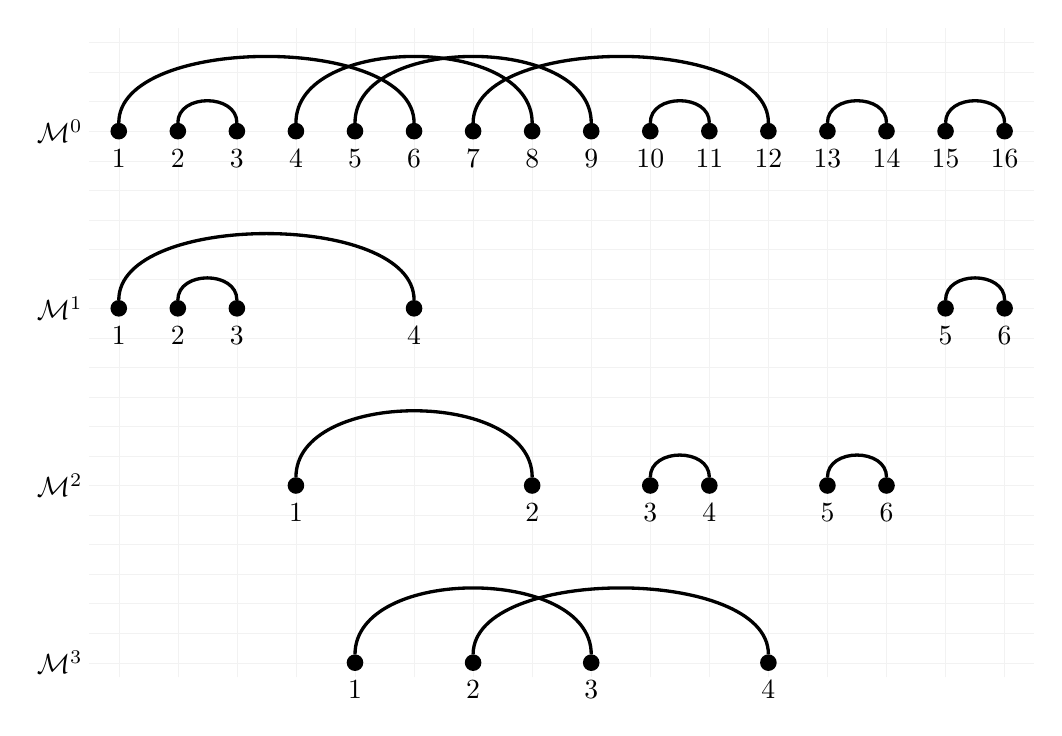
\begin{tikzpicture}
    [
      scale=.75,
      vertex/.style = {circle, fill, minimum size=6pt,inner sep=0pt, outer sep=0pt},
    ]
    \draw[xstep=1,ystep=.5,black,ultra thin,black!5] (0.5,-9.25) grid (16.5,1.75);

    % matching M^0
    \draw (0,0) node {$\mathcal{M}^0$};

    % vertices
    \foreach \x in {1,...,16}
      \node [vertex,label=below:${\x}$] (vM0\x) at (\x,0) {};

    % M^1 occurrence
    \draw [edge] (vM01.north)  ..controls ($(vM01.north) + (0,1.5)$)  and ($(vM06.north) + (0,1.5)$) .. (vM06.north);
    \draw [edge] (vM02.north)  ..controls ($(vM02.north) + (0,0.5)$)  and ($(vM03.north) + (0,0.5)$)  .. (vM03.north);
    \draw [edge] (vM015.north) ..controls ($(vM015.north) + (0,0.5)$) and ($(vM016.north) + (0,0.5)$) .. (vM016.north);

    % M^2 occurrence
    \draw [edge] (vM04.north)  ..controls ($(vM04.north) + (0,1.5)$)   and ($(vM08.north) + (0,1.5)$) .. (vM08.north);
    \draw [edge] (vM010.north) ..controls ($(vM010.north) + (0,0.5)$) and ($(vM011.north) + (0,0.5)$)  .. (vM011.north);
    \draw [edge] (vM013.north) ..controls ($(vM013.north) + (0,0.5)$) and ($(vM014.north) + (0,0.5)$)  .. (vM014.north);

    % M^3 occurrence
    \draw [edge] (vM05.north)  ..controls ($(vM05.north) + (0,1.5)$)   and ($(vM09.north) + (0,1.5)$) .. (vM09.north);
    \draw [edge] (vM07.north)  ..controls ($(vM07.north) + (0,1.5)$)   and ($(vM012.north) + (0,1.5)$)  .. (vM012.north);

    % matching M^1
    \begin{scope}[yshift=-3cm]
      \draw (0,0) node {$\mathcal{M}^1$};

      \foreach \x/\l in {1/1,2/2,3/3,6/4,15/5,16/6}
        \node [vertex,fill=black,label=below:${\l}$] (vM1\l) at (\x,0) {};

      \draw [edge] (vM11.north) ..controls ($(vM11.north) + (0,1.5)$) and ($(vM14.north) + (0,1.5)$) .. (vM14.north);
      \draw [edge] (vM12.north) ..controls ($(vM12.north) + (0,0.5)$) and ($(vM13.north) + (0,0.5)$) .. (vM13.north);
      \draw [edge] (vM15.north) ..controls ($(vM15.north) + (0,0.5)$) and ($(vM16.north) + (0,0.5)$) .. (vM16.north);    
    \end{scope}

    % matching M^2
    \begin{scope}[yshift=-6cm]
      \draw (0,0) node {$\mathcal{M}^2$};

      \foreach \x/\l in {4/1,8/2,10/3,11/4,13/5,14/6}
        \node [vertex,fill=black,label=below:${\l}$] (vM2\l) at (\x,0) {};

      \draw [edge] (vM21.north) ..controls ($(vM21.north) + (0,1.5)$) and ($(vM22.north) + (0,1.5)$) .. (vM22.north);
      \draw [edge] (vM23.north) ..controls ($(vM23.north) + (0,0.5)$) and ($(vM24.north) + (0,0.5)$) .. (vM24.north);
      \draw [edge] (vM25.north) ..controls ($(vM25.north) + (0,0.5)$) and ($(vM26.north) + (0,0.5)$) .. (vM26.north);    
    \end{scope}

    % matching M^3
    \begin{scope}[yshift=-9cm]
      \draw (0,0) node {$\mathcal{M}^3$};

      \foreach \x/\l in {5/1,7/2,9/3,12/4}
        \node [vertex,fill=black,label=below:${\l}$] (vM3\l) at (\x,0) {};

      \draw [edge] (vM31.north) ..controls ($(vM31.north) + (0,1.5)$) and ($(vM33.north) + (0,1.5)$) .. (vM33.north);
      \draw [edge] (vM32.north) ..controls ($(vM32.north) + (0,1.5)$) and ($(vM34.north) + (0,1.5)$) .. (vM34.north);
    \end{scope}

  \end{tikzpicture}
  \caption{\label{fig:matching-merge-example}%
    A positive instance of \textsc{$3$-Merge matching} together with an alignment
    describing a solution.
  }% end caption
\end{figure}



<<<<<<< HEAD
% Merging matchings
%\subsubsection{Merging matchings}
\label{section:Merging matchings}

This section is devoted to proving that the
\textsc{$3$-Merge Matchings} is \NP-complete.

\begin{proposition}
  \label{proposition:3-merge matching is NP-complete}
  \textsc{$3$-Merge Matching} is \NP-complete.
\end{proposition}

\begin{proof}
  We reduce from the \textsc{$3$-Sat} problem, which is known to
  \NP-complete \cite{DBLP:conf/coco/Karp72}.
  Let $\phi = c_1 \wedge c_2 \wedge \cdots \wedge c_m$ be a CNF formula
  defined over the boolean variables $X =\{x_1, x_2, \dots, x_n\}$.
  For every variable $x_{i} \in X$,
  we let $\OCCURRENCE_1(x_{i})$ (resp. $\OCCURRENCE_2(x_{i})$ and $\OCCURRENCE_3(x_{i})$)
  stand for the number of occurrences of the variable $x_{i}$ as the first (resp. second and third)
  literal of a clause.
  Furthermore, we let $\OCCURRENCE(x_{i})$ stand for
  $\OCCURRENCE_1(x_{i}) + 2\,\OCCURRENCE_2(x_{i}) + \OCCURRENCE_3(x_{i})$.
  For any clause $c$, we let $c[i]$ stand for
  $i$-th literal of $c$.

  We define an instance of the \textsc{$3$-matching Coloring} problem by defining a
  target matching $\mathcal{M}{0} = (V^{0}, E^{0})$
  and three matchings
  $\mathcal{M}{1} = (V^{1}, E^{1})$, $\mathcal{M}{2} = (V^{2}, E^{2})$ and $\mathcal{M}{3} = (V^{3}, E^{3})$.
  All matchings $\mathcal{M}{0}$, $\mathcal{M}{1}$, $\mathcal{M}{2}$ and $\mathcal{M}{3}$ are actually composed
  of independent edges so that any connected component is composed of two vertices only.
  The general idea of the reduction is as follows:
  the target matching $\mathcal{M}{0}$ encodes the whole instance
  and $\mathcal{M}{1}$ encodes an assignment of the variable that satisfies all clauses of $\phi$;
  both $\mathcal{M}{2}$ and $\mathcal{M}{3}$ act as garbage collectors by focusing of those edges of $\mathcal{M}{0}$
  that are not part of the satisfying assignment or are structure edges.

  Set $N=m^2$.
  We have divided the presentation of the matchings $\mathcal{M}{0}, \mathcal{M}{1}, \mathcal{M}{2}$ and $\mathcal{M}{3}$.

  % matching \mathcal{M}0
  \medskip
  \textbf{Defining the target matching $\mathcal{M}{0} = (V^{0}, E^{0})$}
  \medskip

  % \begin{mdframed}
    Define
    \begin{alignat*} {2}
      V^{0} &= \texttt{Var}^{0} \cup \texttt{Cls}^{0}
      &\quad&\text{with $\texttt{Var}^{0} < \texttt{Cls}^{0}$,}
      \\
      \texttt{Var}^{0} &= \bigcup_{i=1}^{n} \texttt{Var}^{0}_{i}
      &&\text{with $\texttt{Var}^{0}_1 < \texttt{Var}^{0}_2 < \cdots < \texttt{Var}^{0}_n$,}
      \\
      \texttt{Cls}^{0} &= \bigcup_{j=1}^{m} \texttt{Cls}^{0}_{j}
      &&\text{with $\texttt{Cls}^{0}_1 < \texttt{Cls}^{0}_2 < \cdots < \texttt{Cls}^{0}_m$.}
    \end{alignat*}

    Let us first define the vertices of $\texttt{Var}^{0}$ that correspond
    to the variables $X$.
    Quite naturally, the vertices of $\texttt{Var}^{0}_{i}$, $1 \leq i \leq n$,
    are associated to the boolean variable $x_{i} \in X$.
    For $1 \leq i \leq n$, define
    \begin{alignat*}{2}
      \texttt{Var}^{0}_{i} &=
      &&
      \texttt{T}^{0}_{i,\LEFT} \cup \texttt{T}^{0}_{i,\RIGHT} \cup
      \texttt{F}^{0}_{i,\LEFT} \cup \texttt{F}^{0}_{i,\RIGHT} \cup
      \texttt{Y}^{0}_{i,\LEFT} \cup \texttt{Y}^{0}_{i,\RIGHT} \cup
      \texttt{X}^{0}_{i} \cup \neg\texttt{X}^{0}_{i}
      \\
      \intertext{
      with $$\texttt{T}^{0}_{i,\LEFT} <
      \texttt{Y}^{0}_{i,\LEFT} <
      \texttt{X}^{0}_{i} <
      \texttt{F}^{0}_{i,\LEFT} <
      \texttt{T}^{0}_{i,\RIGHT} <
      \neg\texttt{X}^{0}_{i} <
      \texttt{Y}^{0}_{i,\RIGHT} <
      \texttt{F}^{0}_{i,\RIGHT},$$
      and}
      \texttt{T}^{0}_{i,\LEFT}
      &=
      &&\{\texttt{t}^{0}_{i,j,\LEFT} : 1 \leq j \leq N\}
      \\
      \texttt{Y}^{0}_{i,\LEFT}
      &=
      &&\{\texttt{y}^{0}_{i,j,\LEFT} : 1 \leq j \leq N\}
      \\
      \texttt{X}^{0}_{i}
      &=
      &&\texttt{X}^{0}_{i,1} \cup \texttt{X}^{0}_{i,2} \cup \texttt{X}^{0}_{i,3}
      \\
      \texttt{X}^{0}_{i,1}
      &=
      &&\{\texttt{x}^{0}_{i,1,j} :
      \text{$c_{j}[1] = x_{i}$ or $c_{j}[1] = \overline{x_{i}}$}\}
      \\
      \texttt{X}^{0}_{i,2}
      &=
      &&\{\texttt{x}^{0}_{i,2,j,\FST}, \texttt{x}^{0}_{i,2,j,\SND} :
      \text{$c_{j}[2] = x_{i}$ or $c_{j}[2] = \overline{x_{i}}$}\}
      \\
      \texttt{X}^{0}_{i,3}
      &=
      &&\{\texttt{x}^{0}_{i,3,j} : \text{$c_{j}[3] = x_{i}$ or $c_{j}[3] = \overline{x_{i}}$}\}
      \\
      \texttt{F}^{0}_{i,\LEFT}
      &=
      &&\{\texttt{f}^{0}_{i,j,\LEFT} : 1 \leq j \leq N\}
      \\
      \texttt{T}^{0}_{i,\RIGHT}
      &=
      &&\{\texttt{t}^{0}_{i,j,\RIGHT} : 1 \leq j \leq N\}
      \\
      \neg\texttt{X}^{0}_{i}
      &=
      &&\neg\texttt{X}^{0}_{i,1} \cup \neg\texttt{X}^{0}_{i,2} \cup \neg\texttt{X}^{0}_{i,3}
      \\
      \neg\texttt{X}^{0}_{i,1}
      &=
      &&\{\neg\texttt{x}^{0}_{i,1,j} :
      \text{$c_{j}[1] = x_{i}$ or $c_{j}[1] = \overline{x_{i}}$}\}
      \\
      \neg\texttt{X}^{0}_{i,2}
      &=
      &&\{\neg\texttt{x}^{0}_{i,2,j,\FST}, \texttt{x}^{0}_{i,2,j,\SND} :
      \text{$c_{j}[2] = x_{i}$ or $c_{j}[2] = \overline{x_{i}}$}\}
      \\
      \neg\texttt{X}^{0}_{i,3}
      &=
      &&\{\neg\texttt{x}^{0}_{i,3,j} :
      \text{$c_{j}[3] = x_{i}$ or $c_{j}[3] = \overline{x_{i}}$}\}
      \\
      \texttt{Y}^{0}_{i,\RIGHT}
      &=
      &&\{\texttt{y}^{0}_{i,j,\RIGHT} : 1 \leq j \leq N\}
      \\
      \texttt{F}^{0}_{i,\RIGHT}
      &=
      &&\{\texttt{f}^{0}_{i,j,\RIGHT} : 1 \leq j \leq N\}\text{.}
    \end{alignat*}
    All vertices within subsets
    $\texttt{T}^{0}_{i,\LEFT}, \texttt{t}^{0}_{i,\RIGHT},
    \texttt{F}^{0}_{i,\LEFT}, \texttt{F}^{0}_{i,\RIGHT},
    \texttt{Y}^{0}_{i,\LEFT}, \texttt{Y}^{0}_{i,\RIGHT},
    \texttt{X}^{0}_{i}$ and $\neg\texttt{X}^{0}_{i}$
    are ordered according to their $j$-coordinate.
    Furthermore,
    $\texttt{x}^{0}_{i,2,j,\FST} < \texttt{x}^{0}_{i,2,j,\SND}$
    for $\texttt{x}^{0}_{i,2,j,\FST}, \texttt{x}^{0}_{i,2,j,\SND} \in \texttt{X}^{0}_{i,2}$
    and
    $\neg\texttt{x}^{0}_{i,2,j,\FST} < \neg\texttt{x}^{0}_{i,2,j,\SND}$
    for $\neg\texttt{x}^{0}_{i,2,j,\FST}, \neg\texttt{x}^{0}_{i,2,j,\SND} \in \neg\texttt{X}^{0}_{i,2}$.

    As for the vertices of $\texttt{Cls}^{0}$, for every $1 \leq j \leq m$, define
    \begin{align*}
      \texttt{Cls}^{0}_{j} &=
      \texttt{L}^{0}_{j} \cup
      \texttt{A}^{0}_{j} \cup
      \texttt{B}^{0}_{j} \cup
      \texttt{C}^{0}_{j} \cup
      \texttt{D}^{0}_{j}
      \\
      \texttt{L}^{0}_{j} &= \{
      \texttt{l}^{0}_{j,1,\TRUE},
      \texttt{l}^{0}_{j,1,\FALSE},
      \texttt{l}^{0}_{j,2,\FALSE,\FST},
      \texttt{l}^{0}_{j,2,\TRUE},
      \texttt{l}^{0}_{j,2,\FALSE,\SND},
      \texttt{l}^{0}_{j,3,\FALSE},
      \texttt{l}^{0}_{j,3,\TRUE}
      \}
      \\
      \texttt{A}^{0}_{j} &= \{\texttt{a}^{0}_{j,\LEFT}, \texttt{a}^{0}_{j,\RIGHT}\}
      \\
      \texttt{B}^{0}_{j} &= \{\texttt{b}^{0}_{j,\LEFT}, \texttt{b}^{0}_{j,\RIGHT}\}
      \\
      \texttt{C}^{0}_{j} &= \{\texttt{c}^{0}_{j,\LEFT}, \texttt{c}^{0}_{j,\RIGHT}\}
      \\
      \texttt{D}^{0}_{j} &= \{\texttt{d}^{0}_{j,\LEFT}, \texttt{d}^{0}_{j,\RIGHT}\}
    \end{align*}
    with
    $
    \texttt{l}^{0}_{j,1,\TRUE} <
    \texttt{a}^{0}_{j,\LEFT} <
    \texttt{l}^{0}_{j,1,\FALSE} <
    \texttt{b}^{0}_{j,\LEFT} <
    \texttt{a}^{0}_{j,\RIGHT} <
    \texttt{l}^{0}_{j,2,\FALSE,\FST} <
    \texttt{b}^{0}_{j,\RIGHT} <
    \texttt{l}^{0}_{j,2,\TRUE} <
    \texttt{c}^{0}_{j,\LEFT} <
    \texttt{l}^{0}_{j,2,\FALSE,\SND} <
    \texttt{d}^{0}_{j,\LEFT} <
    \texttt{c}^{0}_{j,\RIGHT} <
    \texttt{l}^{0}_{j,3,\FALSE} <
    \texttt{d}^{0}_{j,\RIGHT} <
    \texttt{l}^{0}_{j,3,\TRUE}
    $.

    We now turn to defining the edges $E^{0}$ of the matching $\mathcal{M}{0}$.
    Define
    \begin{alignat*}{2}
      E^{0} &=&& E^{0}_{\texttt{Var}} \cup E^{0}_{\texttt{Var},\texttt{Cls}} \cup E^{0}_{\texttt{Cls}},
      \\
      E^{0}_{\texttt{Var}} &=&& \bigcup_{i=1}^{n} E^{0}_{\texttt{Var}, i},
      \\
      \forall 1\leq i \leq n,\;
      E^{0}_{\texttt{Var}, i} &=&&
      \bigcup_{k=1}^{N} (\texttt{t}^{0}_{i,k,\LEFT}, \texttt{t}^{0}_{i,N-k+1,\RIGHT})
      \;\cup\;
      \bigcup_{k=1}^{N} (\texttt{f}^{0}_{i,k,\LEFT}, \texttt{f}^{0}_{i,N-k+1,\RIGHT}) \;\cup
      \\
      &&&
      \bigcup_{k=1}^{N} (\texttt{y}^{0}_{i,k,\LEFT}, \texttt{y}^{0}_{i,N-k+1,\RIGHT}),
      \\
      E^{0}_{\texttt{Cls}} &=&& \bigcup_{j=1}^{m} E^{0}_{\texttt{Cls}, j},
      \\
      \forall 1\leq j \leq m,\;
      E^{0}_{\texttt{Cls}, j} &=&&
      \{(\texttt{a}^{0}_{j,\LEFT}, \texttt{a}^{0}_{j,\RIGHT}),
      (\texttt{b}^{0}_{j,\LEFT}, \texttt{b}^{0}_{j,\RIGHT}),
      (\texttt{c}^{0}_{j,\LEFT}, \texttt{c}^{0}_{j,\RIGHT}),
      (\texttt{d}^{0}_{j,\LEFT}, \texttt{d}^{0}_{j,\RIGHT})\}\text{.}
    \end{alignat*}
    For $1 \leq i \leq n$, the edges of $E^{0}_{\texttt{Var}, i}$ connect
    vertices of $\texttt{Var}^{0}_{i}$ only, and
    for $1 \leq j \leq m$, the edges of $E^{0}_{\texttt{Cls}, j}$ connect
    vertices of $\texttt{Cls}^{0}_{j}$ only.
    These edges of $E^{0}_{\texttt{Var}} \cup E^{0}_{\texttt{Cls}}$ are thus called
    \emph{intra-gadget} edges (they live inside gadgets).
    What is left is thus to define the \emph{inter-gadget} edges of
    $E^{0}_{\texttt{Var},\texttt{Cls}}$.
    \begin{itemize}
      \item
      For every $\texttt{l}^{0}_{j, 1, \TRUE} \in V^{0}_{\texttt{Cls}}$,
      we add
      the edge $(\texttt{x}^{0}_{i,1,j}, \texttt{l}^{0}_{j, 1, \TRUE})$
      to $E^{0}_{\texttt{Var},\texttt{Cls}}$
      if $c_{j}[1] = x_{i}$, or
      the edge $(\neg\texttt{x}^{0}_{i,1,j}, \texttt{l}^{0}_{j, 1, \TRUE})$
      to $E^{0}_{\texttt{Var},\texttt{Cls}}$
      if $c_{j}[1] = \overline{x_{i}}$.

      \item
      For every $\texttt{l}^{0}_{j, 1, \FALSE} \in V^{0}_{\texttt{Cls}}$,
      we add
      the edge $(\neg\texttt{x}^{0}_{i,1,j}, \texttt{l}^{0}_{j, 1, \TRUE})$
      to $E^{0}_{\texttt{Var},\texttt{Cls}}$
      $c_{j}[1] = x_{i}$, or
      the edge $(\texttt{x}^{0}_{i,1,j}, \texttt{l}^{0}_{j, 1, \TRUE})$
      to $E^{0}_{\texttt{Var},\texttt{Cls}}$
      $c_{j}[1] = \overline{x_{i}}$.

      \item
      For every $\texttt{l}^{0}_{j, 2, \FALSE, \FST} \in V^{0}_{\texttt{Cls}}$, we add
      the edge $(\neg\texttt{x}^{0}_{i,2,j,\FST}, \texttt{l}^{0}_{j, 2, \FALSE, \FST})$
      to $E^{0}_{\texttt{Var},\texttt{Cls}}$
      $c_{j}[2] = x_{i}$, or
      the edge $(\texttt{x}^{0}_{i,2,j,\FST}, \texttt{l}^{0}_{j, 2, \FALSE, \FST})$
      to $E^{0}_{\texttt{Var},\texttt{Cls}}$
      $c_{j}[2] = \overline{x_{i}}$.

      \item
      For every $\texttt{l}^{0}_{j, 2, \FALSE, \SND} \in V^{0}_{\texttt{Cls}}$, we add
      the edge $(\neg\texttt{x}^{0}_{i,2,j,\SND}, \texttt{l}^{0}_{j, 2, \FALSE, \SND})$
      to $E^{0}_{\texttt{Var},\texttt{Cls}}$
      $c_{j}[2] = x_{i}$, or
      the edge $(\texttt{x}^{0}_{i,2,j,\SND}, \texttt{l}^{0}_{j, 2, \FALSE, \SND})$
      to $E^{0}_{\texttt{Var},\texttt{Cls}}$
      $c_{j}[2] = \overline{x_{i}}$.

      \item
      For every $\texttt{l}^{0}_{j, 3, \TRUE} \in V^{0}_{\texttt{Cls}}$,
      we add
      the edge $(\texttt{x}^{0}_{i,3,j}, \texttt{l}^{0}_{j, 3, \TRUE})$
      to $E^{0}_{\texttt{Var},\texttt{Cls}}$
      $c_{j}[3] = x_{i}$, or
      the edge $(\neg\texttt{x}^{0}_{i,1,j}, \texttt{l}^{0}_{j, 3, \TRUE})$
      to $E^{0}_{\texttt{Var},\texttt{Cls}}$
      $c_{j}[3] = \overline{x_{i}}$.

      \item
      For every $\texttt{l}^{0}_{j, 3, \FALSE} \in V^{0}_{\texttt{Cls}}$,
      we add
      the edge $(\neg\texttt{x}^{0}_{i,3,j}, \texttt{l}^{0}_{j, 3, \TRUE})$
      to $E^{0}_{\texttt{Var},\texttt{Cls}}$
      $c_{j}[3] = x_{i}$, or
      the edge $(\texttt{x}^{0}_{i,3,j}, \texttt{l}^{0}_{j, 3, \TRUE})$
      to $E^{0}_{\texttt{Var},\texttt{Cls}}$
      $c_{j}[3] = \overline{x_{i}}$.
    \end{itemize}
  % \end{mdframed}
  
  \medskip

  The construction of the matching $\mathcal{M}{0}$ is illustrated
  in Figure~\ref{fig-3-linear-graph-splitting-variable-gadget-0} and
  Figure~\ref{fig-3-linear-graph-splitting-clause-gadget-0}.

  \begin{figure}
  \centering

  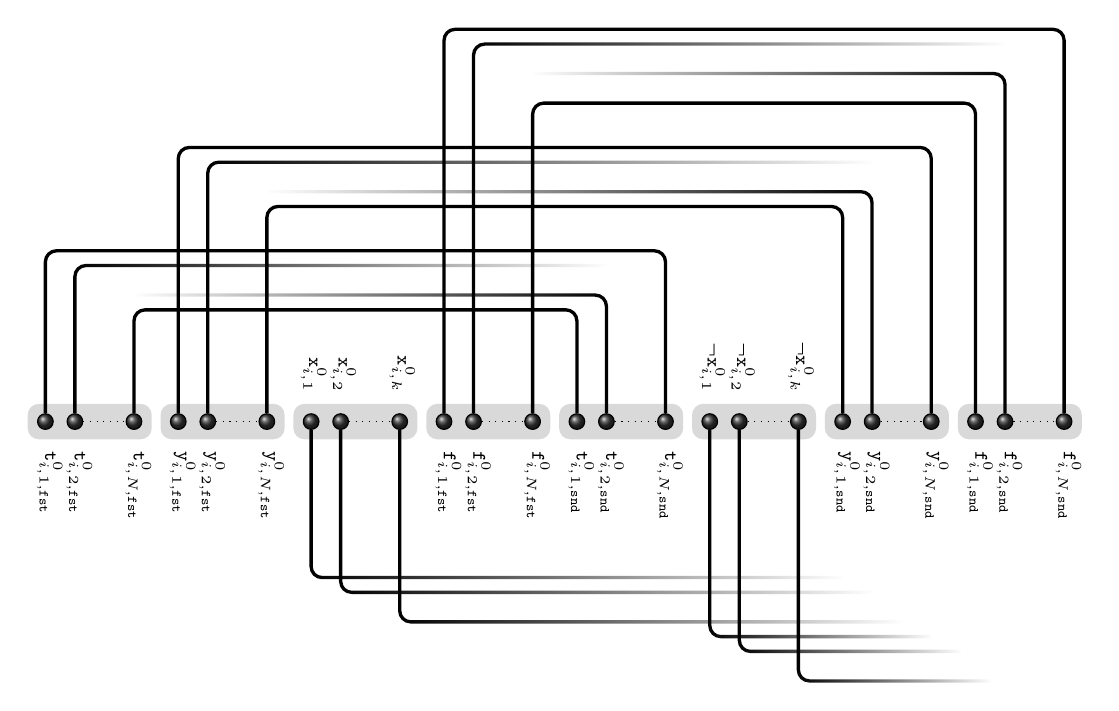
\begin{tikzpicture}
    [
    scale=.375,
    my vertex/.style={basic vertex,
    minimum size=1pt,
    inner sep=2pt,
    ball color=black!80},
    ]
    % vertices

    % p left
    \begin{scope}[]
      \fill [rounded corners, black!15] (-0.6,-0.6) -- (-0.6,0.6) --
      (3.6,0.6)   -- (3.6,-0.6) --
      cycle;
      \node [
      my vertex,
      label={[text depth=0ex,label distance=0.25cm,rotate=-90]right:{\scriptsize $\texttt{t}^{0}_{i,1,\LEFT}$}}
      ] (P1l) at (0,0) {};
      \node [
      my vertex,
      label={[text depth=0ex,label distance=0.25cm,rotate=-90]right:{\scriptsize $\texttt{t}^{0}_{i,2,\LEFT}$}}
      ] (P2l) at (1,0) {};
      \node [
      my vertex,
      label={[text depth=0ex,label distance=0.25cm,rotate=-90]right:{\scriptsize $\texttt{t}^{0}_{i,N,\LEFT}$}}
      ] (PNl) at (3,0) {};
      \path [draw,dotted] (P2l) -- (PNl);
    \end{scope}

    % r left
    \begin{scope}[xshift=4.5cm]
      \fill [rounded corners, black!15] (-0.6,-0.6) -- (-0.6,0.6) --
      (3.6,0.6)   -- (3.6,-0.6) --
      cycle;
      \node [
      my vertex,
      label={[text depth=0ex,label distance=0.25cm,rotate=-90]right:{\scriptsize $\texttt{y}^{0}_{i,1,\LEFT}$}}
      ] (R1l) at (0,0) {};
      \node [
      my vertex,
      label={[text depth=0ex,label distance=0.25cm,rotate=-90]right:{\scriptsize $\texttt{y}^{0}_{i,2,\LEFT}$}}
      ] (R2l) at (1,0) {};
      \node [
      my vertex,
      label={[text depth=0ex,label distance=0.25cm,rotate=-90]right:{\scriptsize $\texttt{y}^{0}_{i,N,\LEFT}$}}
      ] (RNl) at (3,0) {};
      \path [draw,dotted] (R2l) -- (RNl);
    \end{scope}

    % x
    \begin{scope}[xshift=9cm]
      \fill [rounded corners, black!15] (-0.6,-0.6) -- (-0.6,0.6) --
      (3.6,0.6)   -- (3.6,-0.6) --
      cycle;
      \node [
      my vertex,
      label={[text depth=2.5ex,label distance=0.25cm,rotate=-90]left:{\scriptsize $\texttt{x}^{0}_{i,1}$}}
      ] (X1) at (0,0) {};
      \node [
      my vertex,
      label={[text depth=2.5ex,label distance=0.25cm,rotate=-90]left:{\scriptsize $\texttt{x}^{0}_{i,2}$}}
      ] (X2) at (1,0) {};
      \node [
      my vertex,
      label={[text depth=2.5ex,label distance=0.25cm,rotate=-90]left:{\scriptsize $\texttt{x}^{0}_{i,k}$}}
      ] (Xk) at (3,0) {};
      \path [draw,dotted] (X2) -- (Xk);
    \end{scope}

    % q left
    \begin{scope}[xshift=13.5cm]
      \fill [rounded corners, black!15] (-0.6,-0.6) -- (-0.6,0.6) --
      (3.6,0.6)   -- (3.6,-0.6) --
      cycle;
      \node [
      my vertex,
      label={[text depth=0ex,label distance=0.25cm,rotate=-90]right:{\scriptsize $\texttt{f}^{0}_{i,1,\LEFT}$}}
      ] (Q1l) at (0,0) {};
      \node [
      my vertex,
      label={[text depth=0ex,label distance=0.25cm,rotate=-90]right:{\scriptsize $\texttt{f}^{0}_{i,2,\LEFT}$}}
      ] (Q2l) at (1,0) {};
      \node [
      my vertex,
      label={[text depth=0ex,label distance=0.25cm,rotate=-90]right:{\scriptsize $\texttt{f}^{0}_{i,N,\LEFT}$}}
      ] (QNl) at (3,0) {};
      \path [draw,dotted] (Q2l) -- (QNl);
    \end{scope}

    % p right
    \begin{scope}[xshift=18cm]
      \fill [rounded corners, black!15] (-0.6,-0.6) -- (-0.6,0.6) --
      (3.6,0.6)   -- (3.6,-0.6) --
      cycle;
      \node [
      my vertex,
      label={[text depth=0ex,label distance=0.25cm,rotate=-90]right:{\scriptsize $\texttt{t}^{0}_{i,1,\RIGHT}$}}
      ] (P1r) at (0,0) {};
      \node [
      my vertex,
      label={[text depth=0ex,label distance=0.25cm,rotate=-90]right:{\scriptsize $\texttt{t}^{0}_{i,2,\RIGHT}$}}
      ] (P2r) at (1,0) {};
      \node [
      my vertex,
      label={[text depth=0ex,label distance=0.25cm,rotate=-90]right:{\scriptsize $\texttt{t}^{0}_{i,N,\RIGHT}$}}
      ] (PNr) at (3,0) {};
      \path [draw,dotted] (P2r) -- (PNr);
    \end{scope}

    % neg x
    \begin{scope}[xshift=22.5cm]
      \fill [rounded corners, black!15] (-0.6,-0.6) -- (-0.6,0.6) --
      (3.6,0.6)   -- (3.6,-0.6) --
      cycle;
      \node [
      my vertex,
      label={[text depth=2.5ex,label distance=0.25cm,rotate=-90]left:{\scriptsize $\neg\texttt{x}^{0}_{i,1}$}}
      ] (nX1) at (0,0) {};
      \node [
      my vertex,
      label={[text depth=2.5ex,label distance=0.25cm,rotate=-90]left:{\scriptsize $\neg\texttt{x}^{0}_{i,2}$}}
      ] (nX2) at (1,0) {};
      \node [
      my vertex,
      label={[text depth=2.5ex,label distance=0.25cm,rotate=-90]left:{\scriptsize $\neg\texttt{x}^{0}_{i,k}$}}
      ] (nXk) at (3,0) {};
      \path [draw,dotted] (nX2) -- (nXk);
    \end{scope}

    % r right
    \begin{scope}[xshift=27cm]
      \fill [rounded corners, black!15] (-0.6,-0.6) -- (-0.6,0.6) --
      (3.6,0.6)   -- (3.6,-0.6) --
      cycle;
      \node [
      my vertex,
      label={[text depth=0ex,label distance=0.25cm,rotate=-90]right:{\scriptsize $\texttt{y}^{0}_{i,1,\RIGHT}$}}
      ] (R1r) at (0,0) {};
      \node [
      my vertex,
      label={[text depth=0ex,label distance=0.25cm,rotate=-90]right:{\scriptsize $\texttt{y}^{0}_{i,2,\RIGHT}$}}
      ] (R2r) at (1,0) {};
      \node [
      my vertex,
      label={[text depth=0ex,label distance=0.25cm,rotate=-90]right:{\scriptsize $\texttt{y}^{0}_{i,N,\RIGHT}$}}
      ] (RNr) at (3,0) {};
      \path [draw,dotted] (R2r) -- (RNr);
    \end{scope}

    % q right
    \begin{scope}[xshift=31.5cm]
      \fill [rounded corners, black!15] (-0.6,-0.6) -- (-0.6,0.6) --
      (3.6,0.6)   -- (3.6,-0.6) --
      cycle;
      \node [
      my vertex,
      label={[text depth=0ex,label distance=0.25cm,rotate=-90]right:{\scriptsize $\texttt{f}^{0}_{i,1,\RIGHT}$}}
      ] (Q1r) at (0,0) {};
      \node [
      my vertex,
      label={[text depth=0ex,label distance=0.25cm,rotate=-90]right:{\scriptsize $\texttt{f}^{0}_{i,2,\RIGHT}$}}
      ] (Q2r) at (1,0) {};
      \node [
      my vertex,
      label={[text depth=0ex,label distance=0.25cm,rotate=-90]right:{\scriptsize $\texttt{f}^{0}_{i,N,\RIGHT}$}}
      ] (QNr) at (3,0) {};
      \path [draw,dotted] (Q2r) -- (QNr);
    \end{scope}

    % edges
    \path [edge]
    (P1l.north) -- ++(0,5.5) -- ($(PNr.north)+(0,5.5)$) -- (PNr.north);
    \path [edge,path fading=east]
    (P2l.north) -- ++(0,5) --  ($(P2r.north)+(0,5)$);
    \path [edge,path fading=west]
    (P2r.north) -- ++(0,4) -- ($(PNl.north)+(0,4)$);
    \path [edge]
    (PNl.north) -- ($(PNl.north)+(0,3.5)$) -- ($(P1r.north)+(0,3.5)$) -- (P1r.north);

    \path [edge]
    (Q1l.north) -- ++(0,13) -- ($(QNr.north)+(0,13)$) -- (QNr.north);
    \path [edge,path fading=east]
    (Q2l.north) -- ++(0,12.5) --  ($(Q2r.north)+(0,12.5)$);
    \path [edge,path fading=west]
    (Q2r.north) -- ++(0,11.5) -- ($(QNl.north)+(0,11.5)$);
    \path [edge]
    (QNl.north) -- ($(QNl.north)+(0,10.5)$) -- ($(Q1r.north)+(0,10.5)$) -- (Q1r.north);

    \path [edge]
    (R1l.north) -- ++(0,9) -- ($(RNr.north)+(0,9)$) -- (RNr.north);
    \path [edge,path fading=east]
    (R2l.north) -- ++(0,8.5) --  ($(R2r.north)+(0,8.5)$);
    \path [edge,path fading=west]
    (R2r.north) -- ++(0,7.5) -- ($(RNl.north)+(0,7.5)$);
    \path [edge]
    (RNl.north) -- ($(RNl.north)+(0,7)$) -- ($(R1r.north)+(0,7)$) -- (R1r.north);

    \path [edge,path fading=east] (X1.south) -- ++(0,-5) -- ++(18,0);
    \path [edge,path fading=east] (X2.south) -- ++(0,-5.5) -- ++(18,0);
    \path [edge,path fading=east] (Xk.south) -- ++(0,-6.5) -- ++(17,0);

    \path [edge,path fading=east] (nX1.south) -- ++(0,-7) -- ++(7.5,0);
    \path [edge,path fading=east] (nX2.south) -- ++(0,-7.5) -- ++(7.5,0);
    \path [edge,path fading=east] (nXk.south) -- ++(0,-8.5) -- ++(6.5,0);

    %\node [text width=2cm,anchor=west] at (31,-7) {\scriptsize Towards the clause gadgets};
  \end{tikzpicture}

  \caption{\label{fig-3-linear-graph-splitting-variable-gadget-0}%
  A variable gadget $\texttt{Var}^{0}_{i}$ where
  $\texttt{x}^{0}_{i,1}, \texttt{x}^{0}_{i,2}, \dots, \texttt{x}^{0}_{i,k}$
  (resp.
  $\neg\texttt{x}^{0}_{i,1}, \neg\texttt{x}^{0}_{i,2}, \dots, \neg\texttt{x}^{0}_{i,k}$
  )
  represent the vertices of $\texttt{X}^{0}_{i}$ (resp. $\neg\texttt{X}^{0}_{i}$) with
  $k = \OCCURRENCE(x_i) = \OCCURRENCE_1(x_i) + 2\,\OCCURRENCE_2(x_i) + \OCCURRENCE_3(x_i)$.
  The intra-gadget edges of $E^{0}_{\texttt{Var}, i} =
  E^{0}_{\texttt{Var}, i, \texttt{t}} \cup
  E^{0}_{\texttt{Var}, i, \texttt{f}} \cup
  E^{0}_{\texttt{Var}, i, \texttt{y}}$ are shown together
  with the left endpoint parts of the associated inter-gadget edges of
  $E^{0}_{\texttt{Var},\texttt{Cls}}$.
  }% end caption
\end{figure}


  \begin{figure}
  \centering

  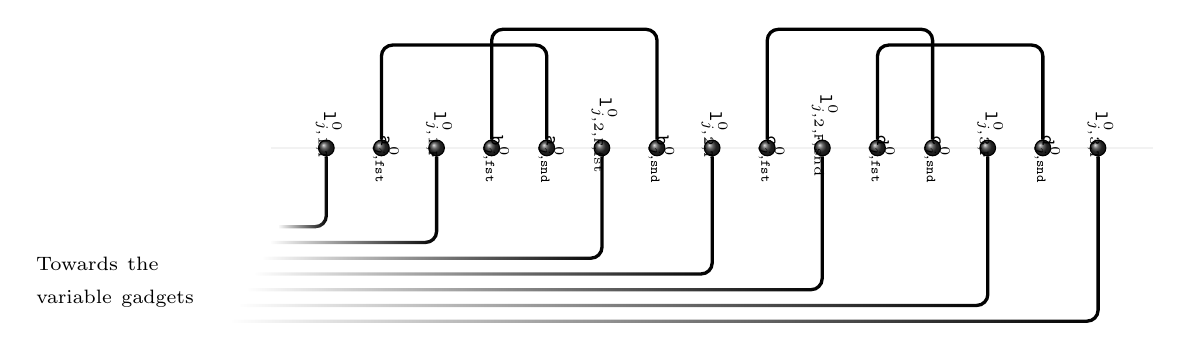
\begin{tikzpicture}
    [
      scale=.2,
      my vertex/.style={basic vertex,
      minimum size=1pt,
      inner sep=2pt,
      ball color=black!80},
    ]
    \path [draw,color=black!5] (0,0) -- (56,0);

    % vertices
    \foreach \i/\l [evaluate=\i as \x using \i*3.5] in
    {
      2/\texttt{a}^{0}_{j,\LEFT},
      4/\texttt{b}^{0}_{j,\LEFT},
      5/\texttt{a}^{0}_{j,\RIGHT},
      7/\texttt{b}^{0}_{j,\RIGHT},
      9/\texttt{c}^{0}_{j,\LEFT},
      11/\texttt{d}^{0}_{j,\LEFT},
      12/\texttt{c}^{0}_{j,\RIGHT},
      14/\texttt{d}^{0}_{j,\RIGHT}
    }
    {
    \node [
    my vertex,
    label={[text depth=0ex,anchor=center,label distance=0.15cm,rotate=-90]right:{\scriptsize $\l$}}
    ] (V\i) at (\x,0) {};
    }
    \foreach \i/\l [evaluate=\i as \x using \i*3.5] in
    {
      1/\texttt{l}^{0}_{j,1,\TRUE},
      3/\texttt{l}^{0}_{j,1,\FALSE},
      6/\texttt{l}^{0}_{j,2,\FALSE,\FST},
      8/\texttt{l}^{0}_{j,2,\TRUE},
      10/\texttt{l}^{0}_{j,2,\FALSE,\SND},
      13/\texttt{l}^{0}_{j,3,\FALSE},
      15/\texttt{l}^{0}_{j,3,\TRUE}
    }
    {

    \node [
      my vertex,
      label={[text depth=2.5ex,anchor=center,label distance=0.15cm,rotate=-90]left:{\scriptsize $\l$}}
    ] (V\i) at (\x,0) {};
    }

    % edges
    \path [edge] (V2.north) -- ++ (0,6) -- ($(V5.north)+(0,6)$) -- (V5.north);
    \path [edge] (V4.north) -- ++ (0,7) -- ($(V7.north)+(0,7)$) -- (V7.north);
    \path [edge] (V9.north) -- ++ (0,7) -- ($(V12.north)+(0,7)$) -- (V12.north);
    \path [edge] (V11.north) -- ++ (0,6) -- ($(V14.north)+(0,6)$) -- (V14.north);

    % incoming edges
    \draw [edge,path fading=west] (V1) -- ++(0,-5) -- +(-3,0) node {};
    \draw [edge,path fading=west] (V3) -- ++(0,-6) -- +(-10.5,0) node {};
    \draw [edge,path fading=west] (V6)  -- ++(0,-7)  -- +(-21.5,0) node {};
    \draw [edge,path fading=west] (V8)  -- ++(0,-8)  -- +(-29,0) node {};
    \draw [edge,path fading=west] (V10) -- ++(0,-9) -- +(-36.5,0) node {};
    \draw [edge,path fading=west] (V13) -- ++(0,-10) -- +(-47.5,0) node {};
    \draw [edge,path fading=west] (V15) -- ++(0,-11) -- +(-55,0) node {};

    \node [text width=2.5cm,anchor=west] at (-15.5,-8.5) {\scriptsize Towards the variable gadgets};

  \end{tikzpicture}

  \caption{\label{fig-3-linear-graph-splitting-clause-gadget-0}%
  A clause gadget $\texttt{Cls}^{0}_{j}$.
  The intra-gadget edges of
  $E^{0}_{\texttt{Cls}, j} =
  E^{0}_{\texttt{Cls}, j, \texttt{a}} \cup
  E^{0}_{\texttt{Cls}, j, \texttt{b}} \cup
  E^{0}_{\texttt{Cls}, j, \texttt{c}} \cup
  E^{0}_{\texttt{Cls}, j, \texttt{d}}$ are shown together
  with the right endpoint parts of the associated inter-gadget edges of
  $E^{0}_{\texttt{Var},\texttt{Cls}}$.
  }% end caption
\end{figure}


  % matching \mathcal{M}1
  \medskip
  \textbf{Defining the target matching $\mathcal{M}{1} = (V^{1}, E^{1})$}
  \medskip
  % \begin{mdframed}
    Define
    \begin{alignat*} {2}
      V^{1} &= \texttt{Var}^{1} \cup \texttt{Cls}^{1}
      &\quad&\text{with $\texttt{Var}^{1} < \texttt{C}^{1}$}
      \\
      \texttt{Var}^{1} &= \bigcup_{i=1}^{n} \texttt{Var}^{1}_{i}
      &&\text{with $\texttt{Var}^{1}_1 < \texttt{Var}^{1}_2 < \cdots < \texttt{Var}^{1}_n$}
      \\
      \texttt{Cls}^{1} &= \bigcup_{j=1}^{m} \texttt{Cls}^{1}_{j}
      &&\text{with $\texttt{Cls}^{1}_1 < \texttt{Cls}^{1}_2 < \cdots < \texttt{Cls}^{1}_m$.}
    \end{alignat*}
    For $1 \leq i \leq n$, define
    \begin{alignat*}{2}
      \texttt{Var}^{1}_{i} &=
      \texttt{TF}^{1}_{i,\LEFT} \cup \texttt{X}^{1}_{i} \cup \texttt{TF}^{1}_{i,\RIGHT}
      &&\text{with $\texttt{TF}^{1}_{i,\LEFT} < \texttt{X}^{1}_{i} < \texttt{TF}^{1}_{i,\RIGHT}$},
      \\
      \texttt{TF}^{1}_{i,\LEFT}
      &=
      \{\texttt{tf}^{1}_{i,j,\LEFT} : 1 \leq j \leq N\},
      &&
      \\
      \texttt{X}^{1}_{i}
      &=
      \{\texttt{x}^{1}_{i,j} : \text{$x_{i}$ or $\overline{x_{i}}$ occurs in clause $c_{j}$}\},
      &&
      \\
      \texttt{TF}^{1}_{i,\RIGHT}
      &=
      \{\texttt{tf}^{1}_{i,j,\RIGHT} : 1 \leq j \leq N\},
      &&
      \\
      \texttt{Cls}^{0}_{j}
      &=
      \{
      \texttt{l}^{1}_{j,1},
      \texttt{l}^{1}_{j,2},
      \texttt{l}^{1}_{j,3},
      \texttt{ab}^{1}_{j,\LEFT},
      \texttt{cd}^{1}_{j,\LEFT},
      \texttt{ab}^{1}_{j,\RIGHT},
      \texttt{cd}^{1}_{j,\RIGHT}
      \}
      &&
    \end{alignat*}
    with
    $
    \texttt{l}^{1}_{j,1} <
    \texttt{ab}^{1}_{j,\LEFT} <
    \texttt{ab}^{1}_{j,\RIGHT} <
    \texttt{l}^{1}_{j,2} <
    \texttt{cd}^{1}_{j,\LEFT} <
    \texttt{cd}^{1}_{j,\RIGHT} <
    \texttt{l}^{1}_{j,3}
    $.
    The vertices in $\texttt{Var}^{1}_{i}$ are ordered according to their second coordinate
    (always written $j$ in the above definitions).

    We now turn to defining the edges $E^{1}$ of the matching $\mathcal{M}{1}$.
    Define
    \begin{align*}
      E^{1} &= E^{1}_{\texttt{Var}} \cup E^{1}_{\texttt{Var},\texttt{Cls}} \cup E^{1}_{\texttt{Cls}},
      \\
      E^{1}_{\texttt{Var}} &= \bigcup_{i=1}^{n} E^{1}_{\texttt{Var}, i},
      \\
      \forall 1\leq i \leq n,\quad
      E^{1}_{\texttt{Var}, i} &= \bigcup_{k=1}^{N} (\texttt{TF}^{1}_{i,k}, \texttt{TF}^{1}_{i,N-k+1}),
      \\
      E^{1}_{\texttt{Cls}} &= \bigcup_{j=1}^{m} E^{1}_{\texttt{Cls}, j},
      \\
      \forall 1\leq j \leq m,\quad
      E^{1}_{\texttt{Cls}, j} &=
      \{
      (\texttt{ab}^{1}_{j,\LEFT}, \texttt{ab}^{1}_{j,\RIGHT}),
      (\texttt{cd}^{1}_{j,\LEFT}, \texttt{cd}^{1}_{j,\RIGHT})
      \}\text{.}
    \end{align*}
    What is left is to define $E^{1}_{\texttt{Var},\texttt{Cls}}$.
    For every $\texttt{l}^{1}_{j, 1} \in V^{1}_{\texttt{Cls}}$
    (resp. $\texttt{l}^{1}_{j, 2} \in V^{1}_{\texttt{Cls}}$ and
    $\texttt{l}^{1}_{j, 3} \in V^{1}_{\texttt{Cls}}$)
    we add
    the edge $(\texttt{x}^{1}_{i,j}, \texttt{l}^{1}_{j, 1})$
    (resp. $(\texttt{x}^{2}_{i,j}, \texttt{l}^{1}_{j, 1})$ and
    $(\texttt{x}^{3}_{i,j}, \texttt{l}^{1}_{j, 1})$)
    to $E^{1}_{\texttt{Var},\texttt{Cls}}$
    if the first (resp. second and third) literal of the clause $c_{j}$
    is the positive or the negative literal $x_{i}$.
  % \end{mdframed}

  The construction of the matching $\mathcal{M}{0}$ is illustrated
  in Figure~\ref{fig-3-linear-graph-splitting-variable-gadget-1} and
  Figure~\ref{fig-3-linear-graph-splitting-clause-gadget-1}.

  \begin{figure}
  \centering

  \begin{tikzpicture}
    [
    scale=.375,
    my vertex/.style={basic vertex,
    minimum size=1pt,
    inner sep=2pt,
    ball color=black!80},
    ]
    % vertices

    % TF left
    \begin{scope}[]
      \fill [rounded corners, black!15] (-0.6,-0.6) -- (-0.6,0.6) --
      (3.6,0.6)   -- (3.6,-0.6) --
      cycle;
      \node [
      my vertex,
      label={[text depth=0ex,label distance=0.25cm,rotate=-90]right:{\scriptsize $\texttt{tf}^{1}_{i,1,\LEFT}$}}
      ] (TF1l) at (0,0) {};
      \node [
      my vertex,
      label={[text depth=0ex,label distance=0.25cm,rotate=-90]right:{\scriptsize $\texttt{tf}^{1}_{i,2,\LEFT}$}}
      ] (TF2l) at (1,0) {};
      \node [
      my vertex,
      label={[text depth=0ex,label distance=0.25cm,rotate=-90]right:{\scriptsize $\texttt{tf}^{1}_{i,N,\LEFT}$}}
      ] (TFNl) at (3,0) {};
      \path [draw,dotted] (TF2l) -- (TFNl);
    \end{scope}

    % x
    \begin{scope}[xshift=4.5cm]
      \fill [rounded corners, black!15] (-0.6,-0.6) -- (-0.6,0.6) --
      (3.6,0.6)   -- (3.6,-0.6) --
      cycle;
      \node [
      my vertex,
      label={[text depth=2.5ex,label distance=0.25cm,rotate=-90]left:{\scriptsize $\texttt{x}^{1}_{i,1}$}}
      ] (X1) at (0,0) {};
      \node [
      my vertex,
      label={[text depth=2.5ex,label distance=0.25cm,rotate=-90]left:{\scriptsize $\texttt{x}^{1}_{i,2}$}}
      ] (X2) at (1,0) {};
      \node [
      my vertex,
      label={[text depth=2.5ex,label distance=0.25cm,rotate=-90]left:{\scriptsize $\texttt{x}^{1}_{i,k}$}}
      ] (Xk) at (3,0) {};
      \path [draw,dotted] (X2) -- (Xk);
    \end{scope}

    % p right
    \begin{scope}[xshift=9cm]
      \fill [rounded corners, black!15] (-0.6,-0.6) -- (-0.6,0.6) --
      (3.6,0.6)   -- (3.6,-0.6) --
      cycle;
      \node [
      my vertex,
      label={[text depth=0ex,label distance=0.25cm,rotate=-90]right:{\scriptsize $\texttt{tf}^{1}_{i,1,\RIGHT}$}}
      ] (TF1r) at (0,0) {};
      \node [
      my vertex,
      label={[text depth=0ex,label distance=0.25cm,rotate=-90]right:{\scriptsize $\texttt{tf}^{1}_{i,2,\RIGHT}$}}
      ] (TF2r) at (1,0) {};
      \node [
      my vertex,
      label={[text depth=0ex,label distance=0.25cm,rotate=-90]right:{\scriptsize $\texttt{tf}^{1}_{i,N,\RIGHT}$}}
      ] (TFNr) at (3,0) {};
      \path [draw,dotted] (TF2r) -- (TFNr);
    \end{scope}

    % edges
    \path [edge]
    (TF1l.north) -- ++(0,5.5) -- ($(TFNr.north)+(0,5.5)$) -- (TFNr.north);
    \path [edge,path fading=east]
    (TF2l.north) -- ++(0,5) --  ($(TF2r.north)+(0,5)$);
    \path [edge,path fading=west]
    (TF2r.north) -- ++(0,4) -- ($(TFNl.north)+(0,4)$);
    \path [edge]
    (TFNl.north) -- ($(PNl.north)+(0,3.5)$) -- ($(TF1r.north)+(0,3.5)$) -- (TF1r.north);

    \path [edge,path fading=east] (X1.south) -- ++(0,-5) -- ++(13,0);
    \path [edge,path fading=east] (X2.south) -- ++(0,-5.5) -- ++(13,0);
    \path [edge,path fading=east] (Xk.south) -- ++(0,-6.5) -- ++(12,0);

    %\node [text width=2cm,anchor=west] at (19,-6) {\scriptsize Towards the clause gadgets};
  \end{tikzpicture}

  \caption{\label{fig-3-linear-graph-splitting-variable-gadget-1}%
  A variable gadget $\texttt{Var}^{1}_{i}$ where
  $\texttt{x}^{1}_{i,1}, \texttt{x}^{1}_{i,2}, \dots, \texttt{x}^{1}_{i,k}$
  represent the vertices of $\texttt{X}^{1}_{i}$ with
  $k = \OCCURRENCE(x_i) = \OCCURRENCE_1(x_i) + 2\,\OCCURRENCE_2(x_i) + \OCCURRENCE_3(x_i)$.
  The intra-gadget edges of $E^{1}_{\texttt{Var}, i} =
  E^{1}_{\texttt{Var}, i, \texttt{tf}} $ are shown together
  with the left endpoint parts of the associated inter-gadget edges of
  $E^{1}_{\texttt{Var},\texttt{Cls}}$.
  }% end caption
\end{figure}


  \begin{figure}
  \centering

  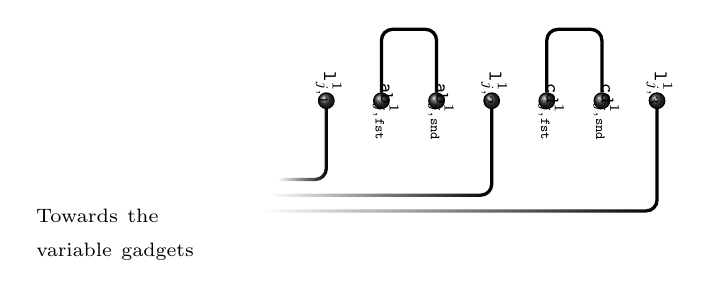
\begin{tikzpicture}
  [
    scale=.2,
    my vertex/.style={basic vertex,
                      minimum size=1pt,
                      inner sep=2pt,
                      ball color=black!80},
  ]
    % vertices
    \foreach \i/\l [evaluate=\i as \x using \i*3.5] in
      {
        2/\texttt{ab}^{1}_{j,\LEFT},
        3/\texttt{ab}^{1}_{j,\RIGHT},
        5/\texttt{cd}^{1}_{j,\LEFT},
        6/\texttt{cd}^{1}_{j,\RIGHT}
      }
    {
    \node [
      my vertex,
      label={[text depth=0ex,anchor=center,label distance=0.15cm,rotate=-90]right:{\scriptsize $\l$}}
    ] (V\i) at (\x,0) {};
    }

    % vertices
    \foreach \i/\l [evaluate=\i as \x using \i*3.5] in
      {
        1/\texttt{l}^{1}_{j,1},
        4/\texttt{l}^{1}_{j,2},
        7/\texttt{l}^{1}_{j,3}
      }
    {
    \node [
      my vertex,
      label={[text depth=2.5ex,anchor=center,label distance=0.15cm,rotate=-90]left:{\scriptsize $\l$}}
    ] (V\i) at (\x,0) {};    }

    % edges
    \path [edge] (V2.north) -- ++ (0,4) -- ($(V3.north)+(0,4)$) -- (V3.north);
    \path [edge] (V5.north) -- ++ (0,4) -- ($(V6.north)+(0,4)$) -- (V6.north);

    % incoming edges
    \draw [edge,path fading=west] (V1) -- ++(0,-5) -- +(-3,0) node {};
    \draw [edge,path fading=west] (V4) -- ++(0,-6) -- +(-14,0) node {};
    \draw [edge,path fading=west] (V7)  -- ++(0,-7)  -- +(-25,0) node {};

    \node [text width=2.5cm,anchor=west] at (-15.5,-8.5) {\scriptsize Towards the variable gadgets};

  \end{tikzpicture}

  \caption{\label{fig-3-linear-graph-splitting-clause-gadget-1}%
    A clause gadget $\texttt{Cls}^{1}_{j}$.
    The two intra-gadget edges of
    $E^{1}_{\texttt{Cls}, j} =
    \{(\texttt{ab}^{1}_{j, \LEFT}, \texttt{ab}^{1}_{j, \RIGHT}),
    (\texttt{cd}^{1}_{j, \LEFT}, \texttt{cd}^{1}_{j, \RIGHT})\}$
    are shown together
    with the right endpoint parts of the associated inter-gadget edges of
    $E^{1}_{\texttt{Var},\texttt{Cls}}$.
  }% end caption
\end{figure}


  % matching \mathcal{M}2
  \medskip
  \textbf{Defining the target matching $\mathcal{M}{2} = (V^{2}, E^{2})$}
  \medskip

  % \begin{mdframed}
    The matching $\mathcal{M}{2}$ is identical to $\mathcal{M}{1}$ except that it does not
    contain any edge in $E^{2}_{\texttt{Cls}}$.
    More formally,
    define
    \begin{alignat*} {2}
      V^{2} &= \texttt{Var}^{2} \cup \texttt{Cls}^{2}
      &\quad&\text{with $\texttt{Var}^{2} < \texttt{Cls}^{2}$}
      \\
      \texttt{Var}^{2} &= \bigcup_{i=1}^{n} \texttt{Var}^{2}_{i}
      &&\text{with $\texttt{Var}^{2}_1 < \texttt{Var}^{2}_2 < \dots < \texttt{Var}^{2}_n$}
      \\
      \texttt{Cls}^{2} &= \bigcup_{j=1}^{m} \texttt{Cls}^{2}_{j}
      &&\text{with $\texttt{Cls}^{2}_1 < \texttt{Cls}^{2}_2 < \dots < \texttt{Cls}^{2}_m$.}
      \\
      \forall, 1 \leq i \leq n,\;
      \texttt{Var}^{2}_{i} &= \texttt{TF}^{2}_{i,\LEFT} \cup \texttt{X}^{2}_{i} \cup \texttt{TF}^{2}_{i,\RIGHT}
      &&\text{with $\texttt{TF}^{2}_{i,\LEFT} < \texttt{X}^{2}_{i} < \texttt{TF}^{2}_{i,\RIGHT}$}
      \\
      \texttt{TF}^{2}_{i,\LEFT}
      &=
      \{\texttt{TF}^{2}_{i,j,\LEFT} : 1 \leq j \leq N\}
      &&\\
      \texttt{X}^{2}_{i}
      &=
      \{\texttt{x}^{2}_{i,j} : \text{$x_{i}$ or $\overline{x_{i}}$ occurs in $c_{j}$}\}
      &&\\
      \texttt{TF}^{2}_{i,\RIGHT}
      &=
      \{\texttt{TF}^{2}_{i,j,\RIGHT} : 1 \leq j \leq N\}
      &&
      \\
      \texttt{Cls}^{2}_{j}
      &=
      \{
      \texttt{l}^{2}_{j,1},
      \texttt{l}^{2}_{j,2},
      \texttt{l}^{2}_{j,3}
      \}
      &&\text{with $\texttt{l}^{2}_{j,1} < \texttt{l}^{2}_{j,2} < \texttt{l}^{2}_{j,3}$}
      \\
    \end{alignat*}
    The vertices in $\texttt{Var}^{2}_{i}$ are ordered according to their second coordinate
    (always written $j$ in the above definitions).

    We now turn to defining the edges $E^{2}$ of the matching $\mathcal{M}{2}$.
    Define
    \begin{align*}
      E^{2} &= E^{2}_{\texttt{Var}} \cup E^{2}_{\texttt{Var},\texttt{Cls}},
      \\
      E^{2}_{\texttt{Var}} &= \bigcup_{i=1}^{n} E^{2}_{\texttt{Var}, i},
      \\
      \forall 1\leq i \leq n,\quad
      E^{2}_{\texttt{Var}, i} &= \bigcup_{k=1}^{N} (\texttt{TF}^{2}_{i,k}, \texttt{TF}^{2}_{i,N-k+1})\text{.}
    \end{align*}
    As for $E^{2}_{\texttt{Var},\texttt{Cls}}$,
    \begin{itemize}
      \item
      for every $\texttt{l}^{2}_{j, 1} \in V^{2}_{\texttt{Cls}}$,
      we add
      the edge $(\texttt{x}^{2}_{i,j}, \texttt{l}^{2}_{j, 1})$
      to $E^{2}_{\texttt{Var},\texttt{Cls}}$
      if $c_{j}[1] = x_{i}$ or $c_{j}[1] = \overline{x_{i}}$.
      \item
      for every $\texttt{l}^{2}_{j, 2} \in V^{2}_{\texttt{Cls}}$,
      we add
      the edge $(\texttt{x}^{2}_{i,j}, \texttt{l}^{2}_{j, 1})$
      to $E^{2}_{\texttt{Var},\texttt{Cls}}$
      if $c_{j}[2] = x_{i}$ or $c_{j}[2] = \overline{x_{i}}$.
      \item
      for every $\texttt{l}^{2}_{j, 3} \in V^{2}_{\texttt{Cls}}$,
      we add
      the edge $(\texttt{x}^{3}_{i,j}, \texttt{l}^{2}_{j, 1})$
      to $E^{2}_{\texttt{Var},\texttt{Cls}}$
      if $c_{j}[3] = x_{i}$ or $c_{j}[3] = \overline{x_{i}}$.
    \end{itemize}
  % \end{mdframed}

  The construction of the matching $\mathcal{M}{2}$ is illustrated
  in Figure~\ref{fig-3-linear-graph-splitting-variable-gadget-2}.

  \begin{figure}
  \centering

  \begin{tikzpicture}
    [
    scale=.375,
    my vertex/.style={basic vertex,
    minimum size=1pt,
    inner sep=2pt,
    ball color=black!80},
    ]
    % vertices

    % TF left
    \begin{scope}[]
      \fill [rounded corners, black!15] (-0.6,-0.6) -- (-0.6,0.6) --
      (3.6,0.6)   -- (3.6,-0.6) --
      cycle;
      \node [
      my vertex,
      label={[text depth=0ex,label distance=0.25cm,rotate=-90]right:{\scriptsize $\texttt{tf}^{2}_{i,1,\LEFT}$}}
      ] (TF1l) at (0,0) {};
      \node [
      my vertex,
      label={[text depth=0ex,label distance=0.25cm,rotate=-90]right:{\scriptsize $\texttt{tf}^{2}_{i,2,\LEFT}$}}
      ] (TF2l) at (1,0) {};
      \node [
      my vertex,
      label={[text depth=0ex,label distance=0.25cm,rotate=-90]right:{\scriptsize $\texttt{tf}^{2}_{i,N,\LEFT}$}}
      ] (TFNl) at (3,0) {};
      \path [draw,dotted] (TF2l) -- (TFNl);
    \end{scope}

    % x
    \begin{scope}[xshift=4.5cm]
      \fill [rounded corners, black!15] (-0.6,-0.6) -- (-0.6,0.6) --
      (3.6,0.6)   -- (3.6,-0.6) --
      cycle;
      \node [
      my vertex,
      label={[text depth=2.5ex,label distance=0.25cm,rotate=-90]left:{\scriptsize $\texttt{x}^{2}_{i,1}$}}
      ] (X1) at (0,0) {};
      \node [
      my vertex,
      label={[text depth=2.5ex,label distance=0.25cm,rotate=-90]left:{\scriptsize $\texttt{x}^{2}_{i,2}$}}
      ] (X2) at (1,0) {};
      \node [
      my vertex,
      label={[text depth=2.5ex,label distance=0.25cm,rotate=-90]left:{\scriptsize $\texttt{x}^{2}_{i,k}$}}
      ] (Xk) at (3,0) {};
      \path [draw,dotted] (X2) -- (Xk);
    \end{scope}

    % p right
    \begin{scope}[xshift=9cm]
      \fill [rounded corners, black!15] (-0.6,-0.6) -- (-0.6,0.6) --
      (3.6,0.6)   -- (3.6,-0.6) --
      cycle;
      \node [
      my vertex,
      label={[text depth=0ex,label distance=0.25cm,rotate=-90]right:{\scriptsize $\texttt{tf}^{2}_{i,1,\RIGHT}$}}
      ] (TF1r) at (0,0) {};
      \node [
      my vertex,
      label={[text depth=0ex,label distance=0.25cm,rotate=-90]right:{\scriptsize $\texttt{tf}^{2}_{i,2,\RIGHT}$}}
      ] (TF2r) at (1,0) {};
      \node [
      my vertex,
      label={[text depth=0ex,label distance=0.25cm,rotate=-90]right:{\scriptsize $\texttt{tf}^{2}_{i,N,\RIGHT}$}}
      ] (TFNr) at (3,0) {};
      \path [draw,dotted] (TF2r) -- (TFNr);
    \end{scope}

    % edges
    \path [edge]
    (TF1l.north) -- ++(0,5.5) -- ($(TFNr.north)+(0,5.5)$) -- (TFNr.north);
    \path [edge,path fading=east]
    (TF2l.north) -- ++(0,5) --  ($(TF2r.north)+(0,5)$);
    \path [edge,path fading=west]
    (TF2r.north) -- ++(0,4) -- ($(TFNl.north)+(0,4)$);
    \path [edge]
    (TFNl.north) -- ($(PNl.north)+(0,3.5)$) -- ($(TF1r.north)+(0,3.5)$) -- (TF1r.north);

    \path [edge,path fading=east] (X1.south) -- ++(0,-5) -- ++(13,0);
    \path [edge,path fading=east] (X2.south) -- ++(0,-5.5) -- ++(13,0);
    \path [edge,path fading=east] (Xk.south) -- ++(0,-6.5) -- ++(12,0);

    %\node [text width=2cm,anchor=west] at (19,-6) {\scriptsize Towards the clause gadgets};
  \end{tikzpicture}

  \caption{\label{fig-3-linear-graph-splitting-variable-gadget-2}%
  A variable gadget $\texttt{Var}^{2}_{i}$ where
  $\texttt{x}^{2}_{i,1}, \texttt{x}^{2}_{i,2}, \dots, \texttt{x}^{2}_{i,k}$
  represent the vertices of $\texttt{X}^{2}_{i}$ with
  $k = \OCCURRENCE(x_i) = \OCCURRENCE_1(x_i) + 2\,\OCCURRENCE_2(x_i) + \OCCURRENCE_3(x_i)$.
  The intra-gadget edges of $E^{2}_{\texttt{Var}, i} =
  E^{2}_{\texttt{Var}, i, \texttt{tf}} $ are shown together
  with the left endpoint parts of the associated inter-gadget edges of
  $E^{2}_{\texttt{Var},\texttt{Cls}}$.
  }% end caption
\end{figure}


  % matching \mathcal{M}3
  \medskip
  \textbf{Defining the target matching $\mathcal{M}{3} = (V^{3}, E^{3})$}
  \medskip

  % \begin{mdframed}
    Define
    \begin{alignat*}{2}
      V^{3} &= \texttt{Var}^{3} \cup \texttt{C}^{3},
      &\quad&\text{$\texttt{Var}^{3} < \texttt{Cls}^{3}$,}
      \\
      \texttt{Var}^{3} &= \bigcup_{i=1}^{n} \texttt{Var}^{3}_{i},
      &&\text{$\texttt{Var}^{3}_1 < \texttt{Var}^{3}_2 < \cdots < \texttt{Var}^{3}_n$,}
      \\
      \texttt{Cls}^{3} &= \bigcup_{j=1}^{m} \texttt{Cls}^{3}_{j},
      &&\text{$\texttt{Cls}^{3}_1 < \texttt{Cls}^{3}_2 < \cdots < \texttt{Cls}^{3}_m$.}
    \end{alignat*}
    where
    \begin{alignat*}{3}
      &\forall \leq i \leq n,\;&
      \texttt{Var}^{3}_{i} &= \texttt{Y}^{3}_{i,\LEFT} \cup \texttt{X}^{3}_{i} \cup \texttt{Y}^{3}_{i,\RIGHT},
      &\quad&\text{$\texttt{Y}^{3}_{i,\LEFT} < \texttt{X}^{3}_{i} < \texttt{Y}^{3}_{i,\RIGHT}$},
      \\
      &\forall \leq i \leq n,\;&
      \texttt{Y}^{3}_{i,\LEFT}
      &=
      \{\texttt{y}^{3}_{i,j,\LEFT} : 1 \leq j \leq N\},
      &&
      \\
      &\forall \leq i \leq n,\;&
      \texttt{X}^{3}_{i}
      &=
      \{\texttt{x}^{3}_{i,j,\FST}, \texttt{x}^{3}_{i,j,\SND} :
      \text{$x_{i} = c_{j}[2]$ or $\overline{x_{i}} = c_{j}[2]$}\},
      &&
      \\
      &\forall \leq i \leq n,\;&
      \texttt{Y}^{3}_{i,\RIGHT}
      &=
      \{\texttt{y}^{3}_{i,j,\RIGHT} : 1 \leq j \leq N\},
      &&
      \\
      &&\texttt{Cls}^{3}_{j}
      &=
      \{
      \texttt{l}^{3}_{j},
      \}
      \cup
      \{
      \texttt{ab}^{3}_{j,\LEFT},
      \texttt{cd}^{3}_{j,\LEFT},
      \texttt{ab}^{3}_{j,\RIGHT},
      \texttt{cd}^{3}_{j,\RIGHT}
      \}
      &&
    \end{alignat*}
    with
    $
    \texttt{ab}^{3}_{j,\LEFT} <
    \texttt{ab}^{3}_{j,\RIGHT} <
    \texttt{l}^{3}_{j} <
    \texttt{cd}^{3}_{j,\LEFT} <
    \texttt{cd}^{3}_{j,1,\RIGHT}
    $.
    All subsets
    $\texttt{Y}^{3}_{i,\LEFT}$, $\texttt{X}^{3}_{i}$ and $\texttt{Y}^{3}_{i,\RIGHT}$,
    are ordered according to the second coordinate index of the vertices
    (always written $j$ in the above definitions).

    For the edges $E^{3}$ of the matching $\mathcal{M}{3}$,
    define
    \begin{alignat*}{2}
      &&
      E^{3} &= E^{3}_{\texttt{Var}} \cup E^{3}_{\texttt{Var},\texttt{Cls}} \cup E^{3}_{\texttt{Cls}}
      \\
      &&
      E^{3}_{\texttt{Var}} &= \bigcup_{i=1}^{n} E^{3}_{\texttt{Var}, i}
      \\
      &\forall 1\leq i \leq n,\quad&
      E^{3}_{\texttt{Var}, 3} &= \bigcup_{k=1}^{N} (\texttt{y}^{3}_{i,k}, \texttt{y}^{3}_{i,N-k+1})
      \\
      &&
      E^{3}_{\texttt{Cls}} &= \bigcup_{j=1}^{m} E^{3}_{\texttt{Cls}, j}
      \\
      &\forall 1\leq j \leq m,\quad&
      E^{3}_{\texttt{Cls}, j} &=
      \{
      (\texttt{ab}^{3}_{j,\LEFT}, \texttt{ab}^{3}_{j,\RIGHT})
      \}\text{.}
    \end{alignat*}
    As for $E^{3}_{\texttt{Var},\texttt{Cls}}$,
    for every $\texttt{l}^{3}_{j} \in \texttt{Cls}^{3}_{j}$,
    we add the edge
    $(\texttt{x}^{3}_{i,j}, \texttt{l}^{3}_{j}) \in E^{3}_{\texttt{Var},\texttt{Cls}}$
    if $x_{i} = c_{j}[2]$ or $\overline{x_{i}} = c_{j}[2]$.
  % \end{mdframed}

  \bigskip

  We now claim that the $3$-CNF formula $\phi$ is satisfiable
  if and only if
  $\mathcal{M}{0}$ is $(\mathcal{M}{1}, \mathcal{M}{2}, \mathcal{M}{3})$-colorable.

  $(\Rightarrow)$
  Suppose that the $3$-CNF formula $\phi$ is satisfiable, and
  let $\gamma : X \to \{\FALSE, \TRUE\}$ be a satisfying assignment
  for $\phi$.
  Let $\COLOR_1$, $\COLOR_2$ and $\COLOR_3$ be three distinct colors.
  We define a mapping
  $\rho : V^{0} \to \{\COLOR_1, \COLOR_2, \COLOR_3\}$ as follows.

  \paragraph*{Gadgets $\texttt{Var}^{0}_{i}$}

  \begin{alignat*}{4}
    &\forall 1 \leq i \leq n, \forall 1 \leq j \leq N\;,
    &\quad
    \rho(\texttt{t}^{0}_{i, j, \LEFT}) &= \rho(\texttt{t}^{0}_{i, j, \RIGHT}) &=&
    \begin{cases}
      \COLOR_1 & \text{if $\gamma(x_i) = \TRUE$}\\
      \COLOR_2 & \text{if $\gamma(x_i) = \FALSE$}
    \end{cases}
    \\
    &\forall 1 \leq i \leq n, \forall 1 \leq j \leq N\;,
    &\quad
    \rho(\texttt{f}^{0}_{i, j, \LEFT}) &= \rho(\texttt{f}^{0}_{i, j, \RIGHT}) &=&
    \begin{cases}
      \COLOR_1 & \text{if $\gamma(x_i) = \FALSE$}\\
      \COLOR_2 & \text{if $\gamma(x_i) = \TRUE$}
    \end{cases}
    \\
    &\forall 1 \leq i \leq n, \forall 1 \leq j \leq N\;,
    &\quad
    \rho(\texttt{y}^{0}_{i, j, \LEFT}) &= \rho(\texttt{y}^{0}_{i, j, \RIGHT}) &=&
    \COLOR_3
    \\
    &\forall 1 \leq i \leq n, \forall 1 \leq j \leq \OCCURRENCE(x_i)\;,
    &\quad
    \rho(\texttt{x}^{0}_{i, 1, j}) &= \rho(\texttt{x}^{0}_{i, 3, j}) &=&
    \begin{cases}
      \COLOR_1 & \text{if $\gamma(x_i) = \TRUE$}\\
      \COLOR_2 & \text{if $\gamma(x_i) = \FALSE$}
    \end{cases}
    \\
    &\forall 1 \leq i \leq n, \forall 1 \leq j \leq \OCCURRENCE(x_i)\;,
    &\quad
    \rho(\neg\texttt{x}^{0}_{i, 1, j}) &= \rho(\neg\texttt{x}^{0}_{i, 3, j}) &=&
    \begin{cases}
      \COLOR_1 & \text{if $\gamma(x_i) = \FALSE$}\\
      \COLOR_2 & \text{if $\gamma(x_i) = \TRUE$}
    \end{cases}
    \\
  \end{alignat*}

  \paragraph*{Gadgets $\texttt{Cls}^{0}_{j}$}

  It can be checked that
  \begin{itemize}
    \item
    every vertex of $\mathcal{M}{0}$ is assigned exactly one color,
    \item
    every edge of $\mathcal{M}{0}$ connect two vertices with the same color,
    \item
    the subgraph of $\mathcal{M}{0}$ induced by color $\COLOR_1$
    (resp. $\COLOR_2$ and $\COLOR_3$) is isomorphic to $\mathcal{M}{1}$
    (resp. $\mathcal{M}{2}$ and $\mathcal{M}{3}$).
  \end{itemize}

  $(\Leftarrow)$
  Suppose now that $\mathcal{M}{0}$ is $(\mathcal{M}{1}, \mathcal{M}{2}, \mathcal{M}{3})$-colorable.
  We show how to construct a satifsying assignment
  $\gamma : X \to \{\FALSE, \TRUE\}$ for $\phi$.


  \begin{figure}
  \centering

  \begin{subfigure}[b]{\textwidth}
    \centering
    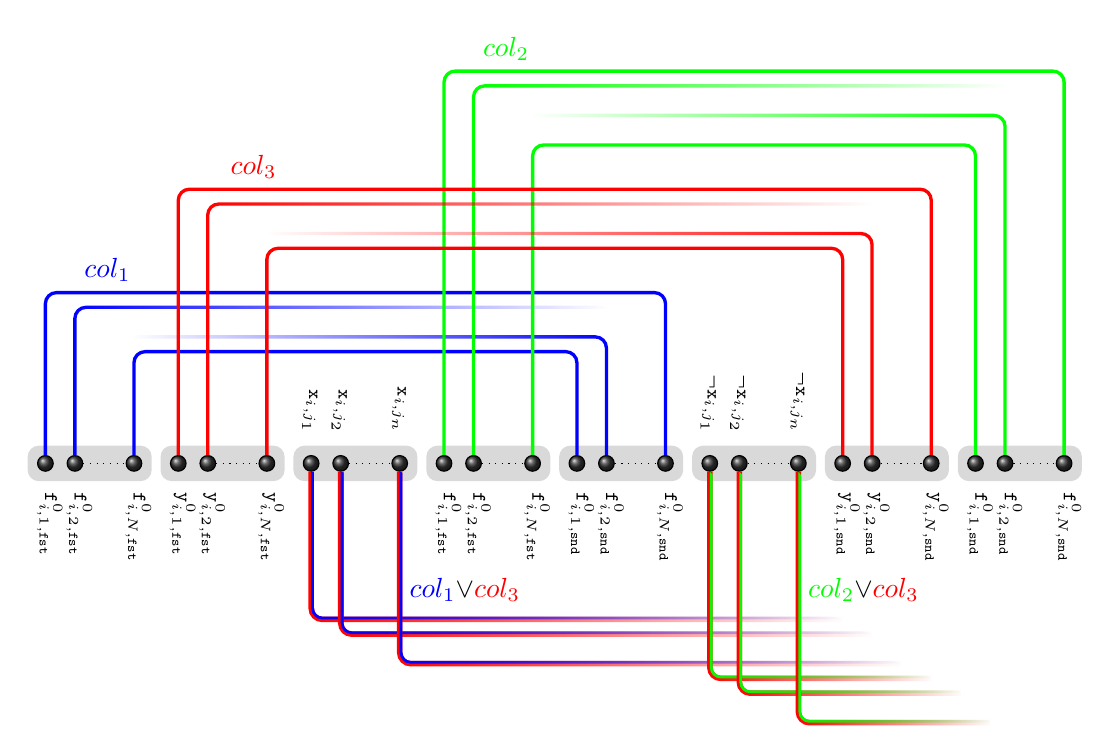
\begin{tikzpicture}
      [
      scale=.375,
      my vertex/.style={basic vertex,
      minimum size=1pt,
      inner sep=2pt,
      ball color=black!80},
      ]
      % vertices

      % p left
      \begin{scope}[]
        \fill [rounded corners, black!15] (-0.6,-0.6) -- (-0.6,0.6) --
        (3.6,0.6)   -- (3.6,-0.6) --
        cycle;
        \node [
        my vertex,
        label={[text depth=-1.75ex,label distance=0.25cm,rotate=-90]right:{\scriptsize $\texttt{f}^0_{i,1,\LEFT}$}}
        ] (T1l) at (0,0) {};
        \node [
        my vertex,
        label={[text depth=-1.75ex,label distance=0.25cm,rotate=-90]right:{\scriptsize $\texttt{f}^0_{i,2,\LEFT}$}}
        ] (T2l) at (1,0) {};
        \node [
        my vertex,
        label={[text depth=-1.75ex,label distance=0.25cm,rotate=-90]right:{\scriptsize $\texttt{f}^0_{i,N,\LEFT}$}}
        ] (TNl) at (3,0) {};
        \path [draw,dotted] (T2l) -- (TNl);
      \end{scope}

      % r left
      \begin{scope}[xshift=4.5cm]
        \fill [rounded corners, black!15] (-0.6,-0.6) -- (-0.6,0.6) --
        (3.6,0.6)   -- (3.6,-0.6) --
        cycle;
        \node [
        my vertex,
        label={[text depth=-1.75ex,label distance=0.25cm,rotate=-90]right:{\scriptsize $\texttt{y}^0_{i,1,\LEFT}$}}
        ] (Y1l) at (0,0) {};
        \node [
        my vertex,
        label={[text depth=-1.75ex,label distance=0.25cm,rotate=-90]right:{\scriptsize $\texttt{y}^0_{i,2,\LEFT}$}}
        ] (Y2l) at (1,0) {};
        \node [
        my vertex,
        label={[text depth=-1.75ex,label distance=0.25cm,rotate=-90]right:{\scriptsize $\texttt{y}^0_{i,N,\LEFT}$}}
        ] (YNl) at (3,0) {};
        \path [draw,dotted] (Y2l) -- (YNl);
      \end{scope}

      % x
      \begin{scope}[xshift=9cm]
        \fill [rounded corners, black!15] (-0.6,-0.6) -- (-0.6,0.6) --
        (3.6,0.6)   -- (3.6,-0.6) --
        cycle;
        \node [
        my vertex,
        label={[text depth=1.75ex,label distance=0.25cm,rotate=-90]left:{\scriptsize $\texttt{x}_{i,j_1}$}}
        ] (X1) at (0,0) {};
        \node [
        my vertex,
        label={[text depth=1.75ex,label distance=0.25cm,rotate=-90]left:{\scriptsize $\texttt{x}_{i,j_2}$}}
        ] (X2) at (1,0) {};
        \node [
        my vertex,
        label={[text depth=1.75ex,label distance=0.25cm,rotate=-90]left:{\scriptsize $\texttt{x}_{i,j_n}$}}
        ] (Xk) at (3,0) {};
        \path [draw,dotted] (X2) -- (Xk);
      \end{scope}

      % q left
      \begin{scope}[xshift=13.5cm]
        \fill [rounded corners, black!15] (-0.6,-0.6) -- (-0.6,0.6) --
        (3.6,0.6)   -- (3.6,-0.6) --
        cycle;
        \node [
        my vertex,
        label={[text depth=-1.75ex,label distance=0.25cm,rotate=-90]right:{\scriptsize $\texttt{f}^0_{i,1,\LEFT}$}}
        ] (F1l) at (0,0) {};
        \node [
        my vertex,
        label={[text depth=-1.75ex,label distance=0.25cm,rotate=-90]right:{\scriptsize $\texttt{f}^0_{i,2,\LEFT}$}}
        ] (F2l) at (1,0) {};
        \node [
        my vertex,
        label={[text depth=-1.75ex,label distance=0.25cm,rotate=-90]right:{\scriptsize $\texttt{f}^0_{i,N,\LEFT}$}}
        ] (FNl) at (3,0) {};
        \path [draw,dotted] (F2l) -- (FNl);
      \end{scope}

      % p right
      \begin{scope}[xshift=18cm]
        \fill [rounded corners, black!15] (-0.6,-0.6) -- (-0.6,0.6) --
        (3.6,0.6)   -- (3.6,-0.6) --
        cycle;
        \node [
        my vertex,
        label={[text depth=-1.75ex,label distance=0.25cm,rotate=-90]right:{\scriptsize $\texttt{f}^0_{i,1,\RIGHT}$}}
        ] (T1r) at (0,0) {};
        \node [
        my vertex,
        label={[text depth=-1.75ex,label distance=0.25cm,rotate=-90]right:{\scriptsize $\texttt{f}^0_{i,2,\RIGHT}$}}
        ] (T2r) at (1,0) {};
        \node [
        my vertex,
        label={[text depth=-1.75ex,label distance=0.25cm,rotate=-90]right:{\scriptsize $\texttt{f}^0_{i,N,\RIGHT}$}}
        ] (TNr) at (3,0) {};
        \path [draw,dotted] (T2r) -- (TNr);
      \end{scope}

      % neg x
      \begin{scope}[xshift=22.5cm]
        \fill [rounded corners, black!15] (-0.6,-0.6) -- (-0.6,0.6) --
        (3.6,0.6)   -- (3.6,-0.6) --
        cycle;
        \node [
        my vertex,
        label={[text depth=1.75ex,label distance=0.25cm,rotate=-90]left:{\scriptsize $\neg\texttt{x}_{i,j_1}$}}
        ] (nX1) at (0,0) {};
        \node [
        my vertex,
        label={[text depth=1.75ex,label distance=0.25cm,rotate=-90]left:{\scriptsize $\neg\texttt{x}_{i,j_2}$}}
        ] (nX2) at (1,0) {};
        \node [
        my vertex,
        label={[text depth=1.75ex,label distance=0.25cm,rotate=-90]left:{\scriptsize $\neg\texttt{x}_{i,j_n}$}}
        ] (nXk) at (3,0) {};
        \path [draw,dotted] (nX2) -- (nXk);
      \end{scope}

      % r right
      \begin{scope}[xshift=27cm]
        \fill [rounded corners, black!15] (-0.6,-0.6) -- (-0.6,0.6) --
        (3.6,0.6)   -- (3.6,-0.6) --
        cycle;
        \node [
        my vertex,
        label={[text depth=-1.75ex,label distance=0.25cm,rotate=-90]right:{\scriptsize $\texttt{y}^0_{i,1,\RIGHT}$}}
        ] (Y1r) at (0,0) {};
        \node [
        my vertex,
        label={[text depth=-1.75ex,label distance=0.25cm,rotate=-90]right:{\scriptsize $\texttt{y}^0_{i,2,\RIGHT}$}}
        ] (Y2r) at (1,0) {};
        \node [
        my vertex,
        label={[text depth=-1.75ex,label distance=0.25cm,rotate=-90]right:{\scriptsize $\texttt{y}^0_{i,N,\RIGHT}$}}
        ] (YNr) at (3,0) {};
        \path [draw,dotted] (Y2r) -- (YNr);
      \end{scope}

      % q right
      \begin{scope}[xshift=31.5cm]
        \fill [rounded corners, black!15] (-0.6,-0.6) -- (-0.6,0.6) --
        (3.6,0.6)   -- (3.6,-0.6) --
        cycle;
        \node [
        my vertex,
        label={[text depth=-1.75ex,label distance=0.25cm,rotate=-90]right:{\scriptsize $\texttt{f}^0_{i,1,\RIGHT}$}}
        ] (F1r) at (0,0) {};
        \node [
        my vertex,
        label={[text depth=-1.75ex,label distance=0.25cm,rotate=-90]right:{\scriptsize $\texttt{f}^0_{i,2,\RIGHT}$}}
        ] (F2r) at (1,0) {};
        \node [
        my vertex,
        label={[text depth=-1.75ex,label distance=0.25cm,rotate=-90]right:{\scriptsize $\texttt{f}^0_{i,N,\RIGHT}$}}
        ] (FNr) at (3,0) {};
        \path [draw,dotted] (F2r) -- (FNr);
      \end{scope}

      % edges
      \path [edge,color=blue]
      (T1l.north) -- ++(0,5.5) -- ($(TNr.north)+(0,5.5)$) node [pos=0.1,above] {$\COLOR_1$} -- (TNr.north);
      \path [edge,color=blue,path fading=east]
      (T2l.north) -- ++(0,5) --  ($(T2r.north)+(0,5)$);
      \path [edge,color=blue,path fading=west]
      (T2r.north) -- ++(0,4) -- ($(TNl.north)+(0,4)$);
      \path [edge,color=blue]
      (TNl.north) -- ($(TNl.north)+(0,3.5)$) -- ($(T1r.north)+(0,3.5)$) -- (T1r.north);

      \path [edge,color=green]
      (F1l.north) -- ++(0,13) -- ($(FNr.north)+(0,13)$) node [pos=0.1,above] {$\COLOR_2$} -- (FNr.north);
      \path [edge,color=green,path fading=east]
      (F2l.north) -- ++(0,12.5) --  ($(F2r.north)+(0,12.5)$);
      \path [edge,color=green,path fading=west]
      (F2r.north) -- ++(0,11.5) -- ($(FNl.north)+(0,11.5)$);
      \path [edge,color=green]
      (FNl.north) -- ($(FNl.north)+(0,10.5)$) -- ($(F1r.north)+(0,10.5)$) -- (F1r.north);

      \path [edge,color=red]
      (Y1l.north) -- ++(0,9) -- ($(YNr.north)+(0,9)$) node [pos=0.1,above] {$\COLOR_3$} -- (YNr.north);
      \path [edge,color=red,path fading=east]
      (Y2l.north) -- ++(0,8.5) --  ($(Y2r.north)+(0,8.5)$);
      \path [edge,color=red,path fading=west]
      (Y2r.north) -- ++(0,7.5) -- ($(YNl.north)+(0,7.5)$);
      \path [edge,color=red]
      (YNl.north) -- ($(YNl.north)+(0,7)$) -- ($(Y1r.north)+(0,7)$) -- (Y1r.north);

      \path [edge,side by side={red}{blue},path fading=east] (X1.south) -- ++(0,-5) -- ++(18,0);
      \path [edge,side by side={red}{blue},path fading=east] (X2.south) -- ++(0,-5.5) -- ++(18,0);
      \path [edge,side by side={red}{blue},path fading=east] (Xk.south) -- ++(0,-6.5) -- ++(17,0);
      \node [text width=2cm] at ($(Xk.south)+(3,-4)$) {$\color{blue}{\COLOR_1} \color{black}{\vee} \color{red}{\COLOR_3}$};

      \path [edge,side by side={red}{green},path fading=east] (nX1.south) -- ++(0,-7) -- ++(7.5,0);
      \path [edge,side by side={red}{green},path fading=east] (nX2.south) -- ++(0,-7.5) -- ++(7.5,0);
      \path [edge,side by side={red}{green},path fading=east] (nXk.south)  -- ++(0,-8.5) -- ++(6.5,0);
      \node [text width=2cm] at ($(nXk.south)+(3,-4)$) {$\color{green}{\COLOR_2} \color{black}{\vee} \color{red}{\COLOR_3}$};

      %\node [text width=2cm,anchor=west] at (31,-7) {\scriptsize Towards the clause gadgets};
    \end{tikzpicture}
    \caption{Setting $\rho(x_i) = \text{true}$ in variable gadget $\texttt{Var}^{0}_{i}$.}
  \end{subfigure}

  \vspace{.5cm}

  \begin{subfigure}[b]{\textwidth}
    \centering
    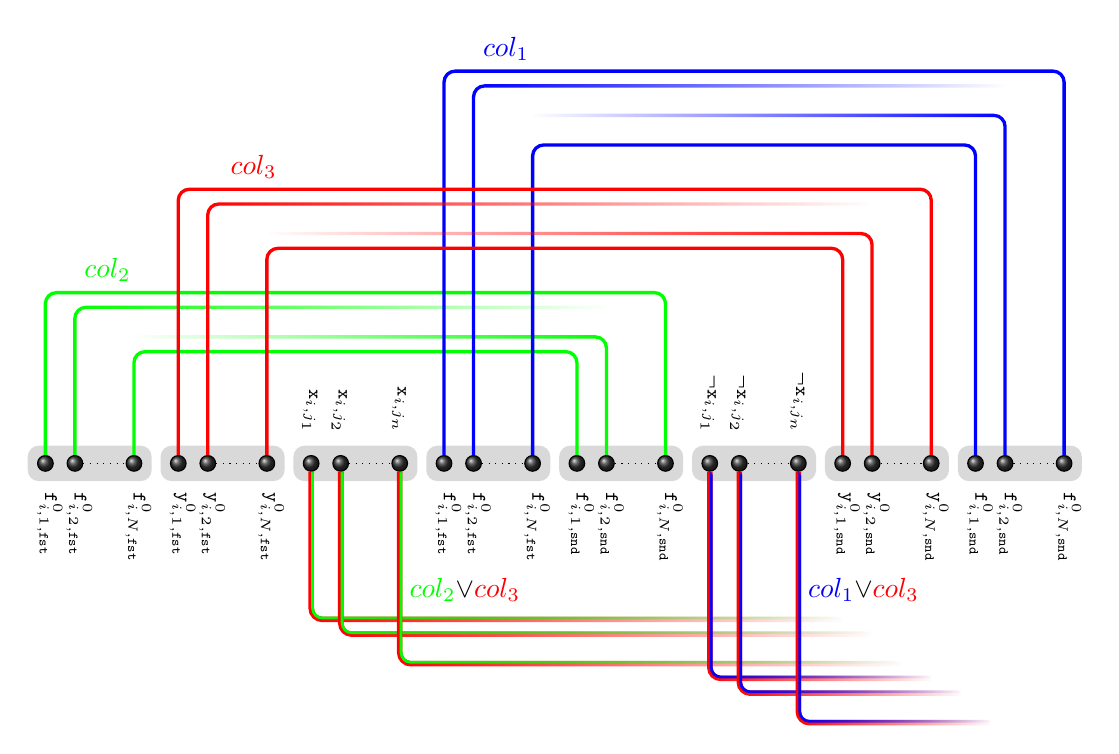
\begin{tikzpicture}
      [
      scale=.375,
      my vertex/.style={basic vertex,
      minimum size=1pt,
      inner sep=2pt,
      ball color=black!80},
      ]
      % vertices

      % p left
      \begin{scope}[]
        \fill [rounded corners, black!15] (-0.6,-0.6) -- (-0.6,0.6) --
        (3.6,0.6)   -- (3.6,-0.6) --
        cycle;
        \node [
        my vertex,
        label={[text depth=-1.75ex,label distance=0.25cm,rotate=-90]right:{\scriptsize $\texttt{f}^0_{i,1,\LEFT}$}}
        ] (T1l) at (0,0) {};
        \node [
        my vertex,
        label={[text depth=-1.75ex,label distance=0.25cm,rotate=-90]right:{\scriptsize $\texttt{f}^0_{i,2,\LEFT}$}}
        ] (T2l) at (1,0) {};
        \node [
        my vertex,
        label={[text depth=-1.75ex,label distance=0.25cm,rotate=-90]right:{\scriptsize $\texttt{f}^0_{i,N,\LEFT}$}}
        ] (TNl) at (3,0) {};
        \path [draw,dotted] (T2l) -- (TNl);
      \end{scope}

      % r left
      \begin{scope}[xshift=4.5cm]
        \fill [rounded corners, black!15] (-0.6,-0.6) -- (-0.6,0.6) --
        (3.6,0.6)   -- (3.6,-0.6) --
        cycle;
        \node [
        my vertex,
        label={[text depth=-1.75ex,label distance=0.25cm,rotate=-90]right:{\scriptsize $\texttt{y}^0_{i,1,\LEFT}$}}
        ] (Y1l) at (0,0) {};
        \node [
        my vertex,
        label={[text depth=-1.75ex,label distance=0.25cm,rotate=-90]right:{\scriptsize $\texttt{y}^0_{i,2,\LEFT}$}}
        ] (Y2l) at (1,0) {};
        \node [
        my vertex,
        label={[text depth=-1.75ex,label distance=0.25cm,rotate=-90]right:{\scriptsize $\texttt{y}^0_{i,N,\LEFT}$}}
        ] (YNl) at (3,0) {};
        \path [draw,dotted] (Y2l) -- (YNl);
      \end{scope}

      % x
      \begin{scope}[xshift=9cm]
        \fill [rounded corners, black!15] (-0.6,-0.6) -- (-0.6,0.6) --
        (3.6,0.6)   -- (3.6,-0.6) --
        cycle;
        \node [
        my vertex,
        label={[text depth=1.75ex,label distance=0.25cm,rotate=-90]left:{\scriptsize $\texttt{x}_{i,j_1}$}}
        ] (X1) at (0,0) {};
        \node [
        my vertex,
        label={[text depth=1.75ex,label distance=0.25cm,rotate=-90]left:{\scriptsize $\texttt{x}_{i,j_2}$}}
        ] (X2) at (1,0) {};
        \node [
        my vertex,
        label={[text depth=1.75ex,label distance=0.25cm,rotate=-90]left:{\scriptsize $\texttt{x}_{i,j_n}$}}
        ] (Xk) at (3,0) {};
        \path [draw,dotted] (X2) -- (Xk);
      \end{scope}

      % q left
      \begin{scope}[xshift=13.5cm]
        \fill [rounded corners, black!15] (-0.6,-0.6) -- (-0.6,0.6) --
        (3.6,0.6)   -- (3.6,-0.6) --
        cycle;
        \node [
        my vertex,
        label={[text depth=-1.75ex,label distance=0.25cm,rotate=-90]right:{\scriptsize $\texttt{f}^0_{i,1,\LEFT}$}}
        ] (F1l) at (0,0) {};
        \node [
        my vertex,
        label={[text depth=-1.75ex,label distance=0.25cm,rotate=-90]right:{\scriptsize $\texttt{f}^0_{i,2,\LEFT}$}}
        ] (F2l) at (1,0) {};
        \node [
        my vertex,
        label={[text depth=-1.75ex,label distance=0.25cm,rotate=-90]right:{\scriptsize $\texttt{f}^0_{i,N,\LEFT}$}}
        ] (FNl) at (3,0) {};
        \path [draw,dotted] (F2l) -- (FNl);
      \end{scope}

      % p right
      \begin{scope}[xshift=18cm]
        \fill [rounded corners, black!15] (-0.6,-0.6) -- (-0.6,0.6) --
        (3.6,0.6)   -- (3.6,-0.6) --
        cycle;
        \node [
        my vertex,
        label={[text depth=-1.75ex,label distance=0.25cm,rotate=-90]right:{\scriptsize $\texttt{f}^0_{i,1,\RIGHT}$}}
        ] (T1r) at (0,0) {};
        \node [
        my vertex,
        label={[text depth=-1.75ex,label distance=0.25cm,rotate=-90]right:{\scriptsize $\texttt{f}^0_{i,2,\RIGHT}$}}
        ] (T2r) at (1,0) {};
        \node [
        my vertex,
        label={[text depth=-1.75ex,label distance=0.25cm,rotate=-90]right:{\scriptsize $\texttt{f}^0_{i,N,\RIGHT}$}}
        ] (TNr) at (3,0) {};
        \path [draw,dotted] (T2r) -- (TNr);
      \end{scope}


      % neg x
      \begin{scope}[xshift=22.5cm]
        \fill [rounded corners, black!15] (-0.6,-0.6) -- (-0.6,0.6) --
        (3.6,0.6)   -- (3.6,-0.6) --
        cycle;
        \node [
        my vertex,
        label={[text depth=1.75ex,label distance=0.25cm,rotate=-90]left:{\scriptsize $\neg\texttt{x}_{i,j_1}$}}
        ] (nX1) at (0,0) {};
        \node [
        my vertex,
        label={[text depth=1.75ex,label distance=0.25cm,rotate=-90]left:{\scriptsize $\neg\texttt{x}_{i,j_2}$}}
        ] (nX2) at (1,0) {};
        \node [
        my vertex,
        label={[text depth=1.75ex,label distance=0.25cm,rotate=-90]left:{\scriptsize $\neg\texttt{x}_{i,j_n}$}}
        ] (nXk) at (3,0) {};
        \path [draw,dotted] (nX2) -- (nXk);
      \end{scope}

      % r right
      \begin{scope}[xshift=27cm]
        \fill [rounded corners, black!15] (-0.6,-0.6) -- (-0.6,0.6) --
        (3.6,0.6)   -- (3.6,-0.6) --
        cycle;
        \node [
        my vertex,
        label={[text depth=-1.75ex,label distance=0.25cm,rotate=-90]right:{\scriptsize $\texttt{y}^0_{i,1,\RIGHT}$}}
        ] (Y1r) at (0,0) {};
        \node [
        my vertex,
        label={[text depth=-1.75ex,label distance=0.25cm,rotate=-90]right:{\scriptsize $\texttt{y}^0_{i,2,\RIGHT}$}}
        ] (Y2r) at (1,0) {};
        \node [
        my vertex,
        label={[text depth=-1.75ex,label distance=0.25cm,rotate=-90]right:{\scriptsize $\texttt{y}^0_{i,N,\RIGHT}$}}
        ] (YNr) at (3,0) {};
        \path [draw,dotted] (Y2r) -- (YNr);
      \end{scope}

      % q right
      \begin{scope}[xshift=31.5cm]
        \fill [rounded corners, black!15] (-0.6,-0.6) -- (-0.6,0.6) --
        (3.6,0.6)   -- (3.6,-0.6) --
        cycle;
        \node [
        my vertex,
        label={[text depth=-1.75ex,label distance=0.25cm,rotate=-90]right:{\scriptsize $\texttt{f}^0_{i,1,\RIGHT}$}}
        ] (F1r) at (0,0) {};
        \node [
        my vertex,
        label={[text depth=-1.75ex,label distance=0.25cm,rotate=-90]right:{\scriptsize $\texttt{f}^0_{i,2,\RIGHT}$}}
        ] (F2r) at (1,0) {};
        \node [
        my vertex,
        label={[text depth=-1.75ex,label distance=0.25cm,rotate=-90]right:{\scriptsize $\texttt{f}^0_{i,N,\RIGHT}$}}
        ] (FNr) at (3,0) {};
        \path [draw,dotted] (F2r) -- (FNr);
      \end{scope}

      % edges
      \path [edge,color=green]
      (T1l.north) -- ++(0,5.5) -- ($(TNr.north)+(0,5.5)$) node [pos=0.1,above] {$\COLOR_2$} -- (TNr.north);
      \path [edge,color=green,path fading=east]
      (T2l.north) -- ++(0,5) --  ($(T2r.north)+(0,5)$);
      \path [edge,color=green,path fading=west]
      (T2r.north) -- ++(0,4) -- ($(TNl.north)+(0,4)$);
      \path [edge,color=green]
      (TNl.north) -- ($(TNl.north)+(0,3.5)$) -- ($(T1r.north)+(0,3.5)$) -- (T1r.north);

      \path [edge,color=blue]
      (F1l.north) -- ++(0,13) -- ($(FNr.north)+(0,13)$) node [pos=0.1,above] {$\COLOR_1$} -- (FNr.north);
      \path [edge,color=blue,path fading=east]
      (F2l.north) -- ++(0,12.5) --  ($(F2r.north)+(0,12.5)$);
      \path [edge,color=blue,path fading=west]
      (F2r.north) -- ++(0,11.5) -- ($(FNl.north)+(0,11.5)$);
      \path [edge,color=blue]
      (FNl.north) -- ($(FNl.north)+(0,10.5)$) -- ($(F1r.north)+(0,10.5)$) -- (F1r.north);

      \path [edge,color=red]
      (Y1l.north) -- ++(0,9) -- ($(YNr.north)+(0,9)$) node [pos=0.1,above] {$\COLOR_3$} -- (YNr.north);
      \path [edge,color=red,path fading=east]
      (Y2l.north) -- ++(0,8.5) --  ($(Y2r.north)+(0,8.5)$);
      \path [edge,color=red,path fading=west]
      (Y2r.north) -- ++(0,7.5) -- ($(YNl.north)+(0,7.5)$);
      \path [edge,color=red]
      (YNl.north) -- ($(YNl.north)+(0,7)$) -- ($(Y1r.north)+(0,7)$) -- (Y1r.north);

      \path [edge,side by side={red}{green},path fading=east] (X1.south) -- ++(0,-5) -- ++(18,0);
      \path [edge,side by side={red}{green},path fading=east] (X2.south) -- ++(0,-5.5) -- ++(18,0);
      \path [edge,side by side={red}{green},path fading=east] (Xk.south) -- ++(0,-6.5) -- ++(17,0);
      \node [text width=2cm] at ($(Xk.south)+(3,-4)$) {$\color{green}{\COLOR_2} \color{black}{\vee} \color{red}{\COLOR_3}$};

      \path [edge,side by side={red}{blue},path fading=east] (nX1.south) -- ++(0,-7) -- ++(7.5,0);
      \path [edge,side by side={red}{blue},path fading=east] (nX2.south) -- ++(0,-7.5) -- ++(7.5,0);
      \path [edge,side by side={red}{blue},path fading=east] (nXk.south) -- ++(0,-8.5) -- ++(6.5,0);
      \node [text width=2cm] at ($(nXk.south)+(3,-4)$) {$\color{blue}{\COLOR_1} \color{black}{\vee} \color{red}{\COLOR_3}$};

      %\node [text width=2cm,anchor=west] at (31,-7) {\scriptsize Towards the clause gadgets};
    \end{tikzpicture}
    \caption{Setting $\rho(x_i) = \text{false}$ in variable gadget $\texttt{Var}^{0}_{i}$.}
  \end{subfigure}
\end{figure}


  
\begin{figure}
  \centering

  \begin{subfigure}[b]{\textwidth}
    \centering
    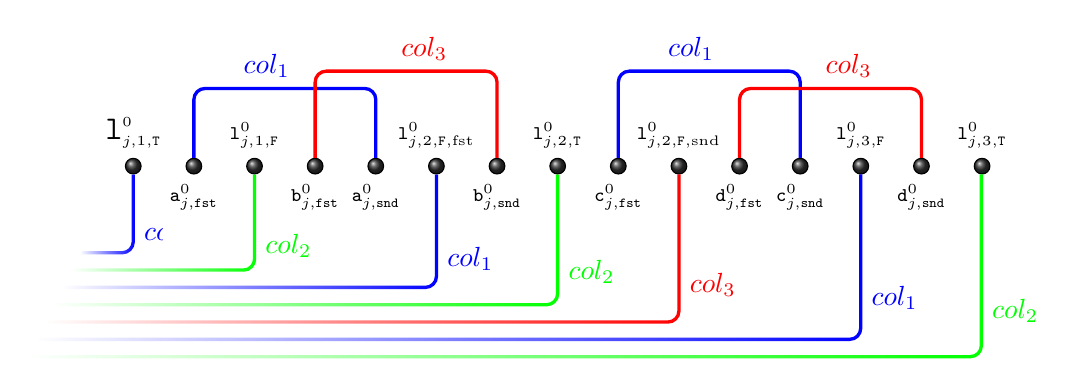
\begin{tikzpicture}
      [
      scale=.22,,,
      my vertex/.style={basic vertex,
      minimum size=1pt,
      inner sep=2pt,
      ball color=black!80},
      ]

      % vertices
      \foreach \i/\o/\l [evaluate=\i as \x using \i*3.5] in
      {
      1/above/\large\texttt{l}^0_{j,1,\TRUE},
      2/below/\texttt{a}^0_{j,\LEFT},
      3/above/\texttt{l}^0_{j,1,\FALSE},
      4/below/\texttt{b}^0_{j,\LEFT},
      5/below/\texttt{a}^0_{j,\RIGHT},
      6/above/\texttt{l}^0_{j,2,\FALSE,\FST},
      7/below/\texttt{b}^0_{j,\RIGHT},
      8/above/\texttt{l}^0_{j,2,\TRUE},
      9/below/\texttt{c}^0_{j,\LEFT},
      10/above/\texttt{l}^0_{j,2,\FALSE,\SND},
      11/below/\texttt{d}^0_{j,\LEFT},
      12/below/\texttt{c}^0_{j,\RIGHT},
      13/above/\texttt{l}^0_{j,3,\FALSE},
      14/below/\texttt{d}^0_{j,\RIGHT},
      15/above/\texttt{l}^0_{j,3,\TRUE}
      }
      {
      \node [my vertex,label=\o:{\scriptsize $\l$}] (V\i) at (\x,0) {};
      }

      % edges
      \path [edge,color=blue] (V2.north) -- ++ (0,4) --
      ($(V5.north)+(0,4)$) node [pos=0.4,above] {$\COLOR_1$} -- (V5.north);

      \path [edge,color=red] (V4.north) -- ++ (0,5) --
      ($(V7.north)+(0,5)$) node [pos=0.6,above] {$\COLOR_3$} -- (V7.north);

      \path [edge,color=blue] (V9.north) -- ++ (0,5) --
      ($(V12.north)+(0,5)$) node [pos=0.4,above] {$\COLOR_1$} -- (V12.north);

      \path [edge,color=red] (V11.north) -- ++ (0,4) --
      ($(V14.north)+(0,4)$) node [pos=0.6,above] {$\COLOR_3$} -- (V14.north);

      % incoming edges


      \draw [edge,color=green,path fading=west] (V3) -- node [pos=0.75,anchor=west] {$\COLOR_2$}
      ++(0,-6) -- +(-10.5,0);

      \draw [edge,color=blue,path fading=west] (V6) -- node [pos=0.75,anchor=west] {$\COLOR_1$}
      ++(0,-7) -- +(-21.5,0);

      \draw [edge,color=green,path fading=west] (V8) -- node [pos=0.75,anchor=west] {$\COLOR_2$}
      ++(0,-8)  -- +(-29,0);

      \draw [edge,color=red,path fading=west] (V10) -- node [pos=0.75,anchor=west] {$\COLOR_3$}
      ++(0,-9) -- +(-36.5,0);

      \draw [edge,color=blue,path fading=west] (V13) -- node [pos=0.75,anchor=west] {$\COLOR_1$}
      ++(0,-10) -- +(-47.5,0);

      \draw [edge,color=green,path fading=west] (V15) -- node [pos=0.75,anchor=west] {$\COLOR_2$}
      ++(0,-11) -- +(-55,0);

      \draw [edge,color=blue,path fading=west] (V1) -- node [pos=0.75,anchor=west] {$\COLOR_1$}
      ++(0,-5) -- +(-3,0);
      %\node [text width=2.5cm,anchor=west] at (-15.5,-8.5) {\scriptsize Towards the variable gadgets};

    \end{tikzpicture}
    \caption{%
    Clause gadget $\texttt{Cls}^{0}_{j}$ for clause $(\ell_{j,1} \vee \ell_{j,2} \vee \ell_{j,3})$
    in case the literals $\ell_{j,1}$, $\ell_{j,2}$ and $\ell_{j,3}$ evaluate to true, false and false,
    respectivelly, according to the satisfying assignment $f$.
    }% end caption  \end{subfigure}
  \end{subfigure}

  \vspace{.5cm}

  \begin{subfigure}[b]{\textwidth}
    \centering
    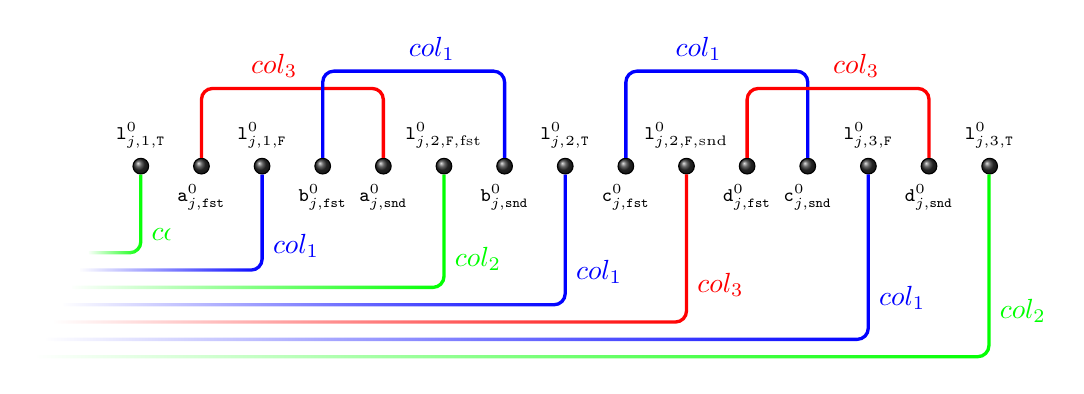
\begin{tikzpicture}
      [
      scale=.22,,,
      my vertex/.style={basic vertex,
      minimum size=1pt,
      inner sep=2pt,
      ball color=black!80},
      ]

      % vertices
      \foreach \i/\o/\l [evaluate=\i as \x using \i*3.5] in
      {
      1/above/\texttt{l}^0_{j,1,\TRUE},
      2/below/\texttt{a}^0_{j,\LEFT},
      3/above/\texttt{l}^0_{j,1,\FALSE},
      4/below/\texttt{b}^0_{j,\LEFT},
      5/below/\texttt{a}^0_{j,\RIGHT},
      6/above/\texttt{l}^0_{j,2,\FALSE,\FST},
      7/below/\texttt{b}^0_{j,\RIGHT},
      8/above/\texttt{l}^0_{j,2,\TRUE},
      9/below/\texttt{c}^0_{j,\LEFT},
      10/above/\texttt{l}^0_{j,2,\FALSE,\SND},
      11/below/\texttt{d}^0_{j,\LEFT},
      12/below/\texttt{c}^0_{j,\RIGHT},
      13/above/\texttt{l}^0_{j,3,\FALSE},
      14/below/\texttt{d}^0_{j,\RIGHT},
      15/above/\texttt{l}^0_{j,3,\TRUE}
      }
      {
      \node [my vertex,label=\o:{\scriptsize $\l$}] (V\i) at (\x,0) {};
      }

      % edges
      \path [edge,color=red] (V2.north) -- ++ (0,4) --
      ($(V5.north)+(0,4)$) node [pos=0.4,above] {$\COLOR_3$}  -- (V5.north);

      \path [edge,color=blue] (V4.north) -- ++ (0,5) --
      ($(V7.north)+(0,5)$) node [pos=0.6,above] {$\COLOR_1$} -- (V7.north);

      \path [edge,color=blue] (V9.north) -- ++ (0,5) --
      ($(V12.north)+(0,5)$) node [pos=0.4,above] {$\COLOR_1$} -- (V12.north);

      \path [edge,color=red] (V11.north) -- ++ (0,4) --
      ($(V14.north)+(0,4)$) node [pos=0.6,above] {$\COLOR_3$} -- (V14.north);

      % incoming edges
      \draw [edge,color=green,path fading=west] (V1) -- node [pos=0.75,anchor=west] {$\COLOR_2$}
      ++(0,-5) -- +(-3,0) node {};

      \draw [edge,color=blue,path fading=west] (V3) -- node [pos=0.75,anchor=west] {$\COLOR_1$}
      ++(0,-6) -- +(-10.5,0) node {};

      \draw [edge,color=green,path fading=west] (V6)  -- node [pos=0.75,anchor=west] {$\COLOR_2$}
      ++(0,-7)  -- +(-21.5,0) node {};

      \draw [edge,color=blue,path fading=west] (V8)  -- node [pos=0.75,anchor=west] {$\COLOR_1$}
      ++(0,-8)  -- +(-29,0) node {};

      \draw [edge,color=red,path fading=west] (V10) -- node [pos=0.75,anchor=west] {$\COLOR_3$}
      ++(0,-9) -- +(-36.5,0) node {};

      \draw [edge,color=blue,path fading=west] (V13) -- node [pos=0.75,anchor=west] {$\COLOR_1$}
      ++(0,-10) -- +(-47.5,0) node {};

      \draw [edge,color=green,path fading=west] (V15) -- node [pos=0.75,anchor=west] {$\COLOR_2$}
      ++(0,-11) -- +(-55,0) node {};

      %\node [text width=2.5cm,anchor=west] at (-15.5,-8.5) {\scriptsize Towards the variable gadgets};

    \end{tikzpicture}
    \caption{%
    Clause gadget $\texttt{Cls}^{0}_{j}$ for clause $(\ell_{j,1} \vee \ell_{j,2} \vee \ell_{j,3})$
    in case the literals $\ell_{j,1}$, $\ell_{j,2}$ and $\ell_{j,3}$ evaluate to false, true and false,
    respectivelly, according to the satisfying assignment $f$.
    }% end caption  \end{subfigure}
  \end{subfigure}

  \vspace{.5cm}

  \begin{subfigure}[b]{\textwidth}
    \centering
    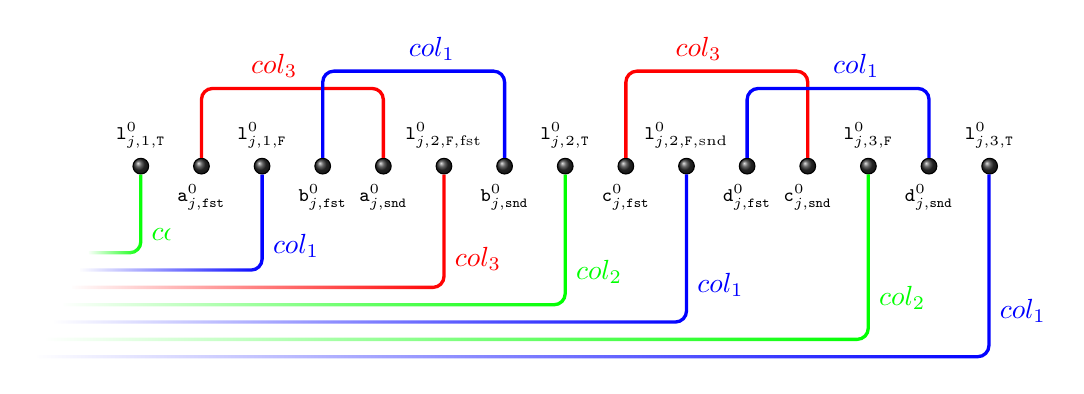
\begin{tikzpicture}
      [
      scale=.22,,,
      my vertex/.style={basic vertex,
      minimum size=1pt,
      inner sep=2pt,
      ball color=black!80},
      ]

      % vertices
      \foreach \i/\o/\l [evaluate=\i as \x using \i*3.5] in
      {
      1/above/\texttt{l}^0_{j,1,\TRUE},
      2/below/\texttt{a}^0_{j,\LEFT},
      3/above/\texttt{l}^0_{j,1,\FALSE},
      4/below/\texttt{b}^0_{j,\LEFT},
      5/below/\texttt{a}^0_{j,\RIGHT},
      6/above/\texttt{l}^0_{j,2,\FALSE,\FST},
      7/below/\texttt{b}^0_{j,\RIGHT},
      8/above/\texttt{l}^0_{j,2,\TRUE},
      9/below/\texttt{c}^0_{j,\LEFT},
      10/above/\texttt{l}^0_{j,2,\FALSE,\SND},
      11/below/\texttt{d}^0_{j,\LEFT},
      12/below/\texttt{c}^0_{j,\RIGHT},
      13/above/\texttt{l}^0_{j,3,\FALSE},
      14/below/\texttt{d}^0_{j,\RIGHT},
      15/above/\texttt{l}^0_{j,3,\TRUE}
      }
      {
      \node [my vertex,label=\o:{\scriptsize $\l$}] (V\i) at (\x,0) {};
      }

      % edges
      \path [edge,color=red] (V2.north) -- ++ (0,4) --
      ($(V5.north)+(0,4)$) node [pos=0.4,above] {$\COLOR_3$}   -- (V5.north);

      \path [edge,color=blue] (V4.north) -- ++ (0,5) --
      ($(V7.north)+(0,5)$) node [pos=0.6,above] {$\COLOR_1$} -- (V7.north);

      \path [edge,color=red] (V9.north) -- ++ (0,5) --
      ($(V12.north)+(0,5)$) node [pos=0.4,above] {$\COLOR_3$} -- (V12.north);

      \path [edge,color=blue] (V11.north) -- ++ (0,4) --
      ($(V14.north)+(0,4)$) node [pos=0.6,above] {$\COLOR_1$} -- (V14.north);

      % incoming edges
      \draw [edge,color=green,path fading=west] (V1) -- node [pos=0.75,anchor=west] {$\COLOR_2$}
      ++(0,-5) -- +(-3,0) node {};

      \draw [edge,color=blue,path fading=west] (V3) -- node [pos=0.75,anchor=west] {$\COLOR_1$}
      ++(0,-6) -- +(-10.5,0) node {};

      \draw [edge,color=red,path fading=west] (V6)  -- node [pos=0.75,anchor=west] {$\COLOR_3$}
      ++(0,-7)  -- +(-21.5,0) node {};

      \draw [edge,color=green,path fading=west] (V8)  -- node [pos=0.75,anchor=west] {$\COLOR_2$}
      ++(0,-8)  -- +(-29,0) node {};

      \draw [edge,color=blue,path fading=west] (V10) -- node [pos=0.75,anchor=west] {$\COLOR_1$}
      ++(0,-9) -- +(-36.5,0) node {};

      \draw [edge,color=green,path fading=west] (V13) -- node [pos=0.75,anchor=west] {$\COLOR_2$}
      ++(0,-10) -- +(-47.5,0) node {};

      \draw [edge,color=blue,path fading=west] (V15) -- node [pos=0.75,anchor=west] {$\COLOR_1$}
      ++(0,-11) -- +(-55,0) node {};

      %\node [text width=2.5cm,anchor=west] at (-15.5,-8.5) {\scriptsize Towards the variable gadgets};

    \end{tikzpicture}
    \caption{%
    Clause gadget $\texttt{Cls}^{0}_{j}$ for clause $(\ell_{j,1} \vee \ell_{j,2} \vee \ell_{j,3})$
    in case the literals $\ell_{j,1}$, $\ell_{j,2}$ and $\ell_{j,3}$ evaluate to false, false and true,
    respectivelly, according to the satisfying assignment $f$.
    }% end caption  \end{subfigure}
  \end{subfigure}

  \vspace{.5cm}

  \begin{subfigure}[b]{\textwidth}
    \centering
    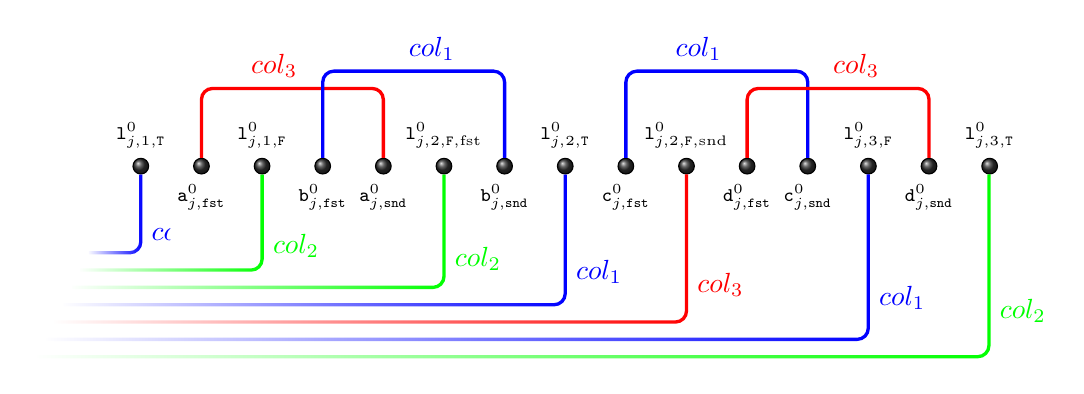
\begin{tikzpicture}
      [
      scale=.22,,,
      my vertex/.style={basic vertex,
      minimum size=1pt,
      inner sep=2pt,
      ball color=black!80},
      ]

      % vertices
      \foreach \i/\o/\l [evaluate=\i as \x using \i*3.5] in
      {
      1/above/\texttt{l}^0_{j,1,\TRUE},
      2/below/\texttt{a}^0_{j,\LEFT},
      3/above/\texttt{l}^0_{j,1,\FALSE},
      4/below/\texttt{b}^0_{j,\LEFT},
      5/below/\texttt{a}^0_{j,\RIGHT},
      6/above/\texttt{l}^0_{j,2,\FALSE,\FST},
      7/below/\texttt{b}^0_{j,\RIGHT},
      8/above/\texttt{l}^0_{j,2,\TRUE},
      9/below/\texttt{c}^0_{j,\LEFT},
      10/above/\texttt{l}^0_{j,2,\FALSE,\SND},
      11/below/\texttt{d}^0_{j,\LEFT},
      12/below/\texttt{c}^0_{j,\RIGHT},
      13/above/\texttt{l}^0_{j,3,\FALSE},
      14/below/\texttt{d}^0_{j,\RIGHT},
      15/above/\texttt{l}^0_{j,3,\TRUE}
      }
      {
      \node [my vertex,label=\o:{\scriptsize $\l$}] (V\i) at (\x,0) {};
      }

      % edges
      \path [edge,color=red] (V2.north) -- ++ (0,4) --
      ($(V5.north)+(0,4)$) node [pos=0.4,above] {$\COLOR_3$} -- (V5.north);

      \path [edge,color=blue] (V4.north) -- ++ (0,5) --
      ($(V7.north)+(0,5)$) node [pos=0.6,above] {$\COLOR_1$} -- (V7.north);

      \path [edge,color=blue] (V9.north) -- ++ (0,5) --
      ($(V12.north)+(0,5)$) node [pos=0.4,above] {$\COLOR_1$} -- (V12.north);

      \path [edge,color=red] (V11.north) -- ++ (0,4) --
      ($(V14.north)+(0,4)$) node [pos=0.6,above] {$\COLOR_3$} -- (V14.north);

      % incoming edges
      \draw [edge,color=blue,path fading=west] (V1) -- node [pos=0.75,anchor=west] {$\COLOR_1$}
      ++(0,-5) -- +(-3,0) node {};

      \draw [edge,color=green,path fading=west] (V3) -- node [pos=0.75,anchor=west] {$\COLOR_2$}
      ++(0,-6) -- +(-10.5,0) node {};

      \draw [edge,color=green,path fading=west] (V6)  -- node [pos=0.75,anchor=west] {$\COLOR_2$}
      ++(0,-7)  -- +(-21.5,0) node {};

      \draw [edge,color=blue,path fading=west] (V8)  -- node [pos=0.75,anchor=west] {$\COLOR_1$}
      ++(0,-8)  -- +(-29,0) node {};

      \draw [edge,color=red,path fading=west] (V10) --  node [pos=0.75,anchor=west] {$\COLOR_3$}
      ++(0,-9) -- +(-36.5,0) node {};

      \draw [edge,color=blue,path fading=west] (V13) -- node [pos=0.75,anchor=west] {$\COLOR_1$}
      ++(0,-10) -- +(-47.5,0) node {};

      \draw [edge,color=green,path fading=west] (V15) -- node [pos=0.75,anchor=west] {$\COLOR_2$}
      ++(0,-11) -- +(-55,0) node {};

      %\node [text width=2.5cm,anchor=west] at (-15.5,-8.5) {\scriptsize Towards the variable gadgets};

    \end{tikzpicture}
    \caption{%
    Clause gadget $\texttt{Cls}^{0}_{j}$ for clause $(\ell_{j,1} \vee \ell_{j,2} \vee \ell_{j,3})$
    in case the literals $\ell_{j,1}$, $\ell_{j,2}$ and $\ell_{j,3}$ evaluate to true, true and false,
    respectivelly, according to the satisfying assignment $f$.
    }% end caption  \end{subfigure}
  \end{subfigure}

\end{figure}

\begin{figure}\ContinuedFloat

  \begin{subfigure}[b]{\textwidth}
    \centering
    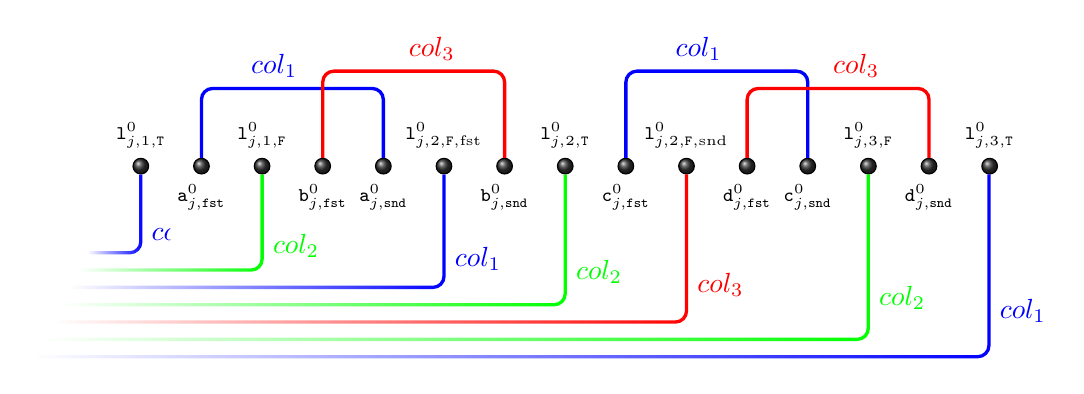
\begin{tikzpicture}
      [
      scale=.22,,,
      my vertex/.style={basic vertex,
      minimum size=1pt,
      inner sep=2pt,
      ball color=black!80},
      ]

      % vertices
      \foreach \i/\o/\l [evaluate=\i as \x using \i*3.5] in
      {
      1/above/\texttt{l}^0_{j,1,\TRUE},
      2/below/\texttt{a}^0_{j,\LEFT},
      3/above/\texttt{l}^0_{j,1,\FALSE},
      4/below/\texttt{b}^0_{j,\LEFT},
      5/below/\texttt{a}^0_{j,\RIGHT},
      6/above/\texttt{l}^0_{j,2,\FALSE,\FST},
      7/below/\texttt{b}^0_{j,\RIGHT},
      8/above/\texttt{l}^0_{j,2,\TRUE},
      9/below/\texttt{c}^0_{j,\LEFT},
      10/above/\texttt{l}^0_{j,2,\FALSE,\SND},
      11/below/\texttt{d}^0_{j,\LEFT},
      12/below/\texttt{c}^0_{j,\RIGHT},
      13/above/\texttt{l}^0_{j,3,\FALSE},
      14/below/\texttt{d}^0_{j,\RIGHT},
      15/above/\texttt{l}^0_{j,3,\TRUE}
      }
      {
      \node [my vertex,label=\o:{\scriptsize $\l$}] (V\i) at (\x,0) {};
      }

      % edges
      \path [edge,color=blue] (V2.north) -- ++ (0,4) --
      ($(V5.north)+(0,4)$) node [pos=0.4,above] {$\COLOR_1$} -- (V5.north);

      \path [edge,color=red] (V4.north) -- ++ (0,5) --
      ($(V7.north)+(0,5)$) node [pos=0.6,above] {$\COLOR_3$} -- (V7.north);

      \path [edge,color=blue] (V9.north) -- ++ (0,5) --
      ($(V12.north)+(0,5)$) node [pos=0.4,above] {$\COLOR_1$} -- (V12.north);

      \path [edge,color=red] (V11.north) -- ++ (0,4) --
      ($(V14.north)+(0,4)$) node [pos=0.6,above] {$\COLOR_3$} -- (V14.north);

      % incoming edges
      \draw [edge,color=blue,path fading=west] (V1) -- node [pos=0.75,anchor=west] {$\COLOR_1$}
      ++(0,-5) -- +(-3,0) node {};

      \draw [edge,color=green,path fading=west] (V3) -- node [pos=0.75,anchor=west] {$\COLOR_2$}
      ++(0,-6) -- +(-10.5,0) node {};

      \draw [edge,color=blue,path fading=west] (V6)  -- node [pos=0.75,anchor=west] {$\COLOR_1$}
      ++(0,-7)  -- +(-21.5,0) node {};

      \draw [edge,color=green,path fading=west] (V8)  -- node [pos=0.75,anchor=west] {$\COLOR_2$}
      ++(0,-8)  -- +(-29,0) node {};

      \draw [edge,color=red,path fading=west] (V10) -- node [pos=0.75,anchor=west] {$\COLOR_3$}
      ++(0,-9) -- +(-36.5,0) node {};

      \draw [edge,color=green,path fading=west] (V13) -- node [pos=0.75,anchor=west] {$\COLOR_2$}
      ++(0,-10) -- +(-47.5,0) node {};

      \draw [edge,color=blue,path fading=west] (V15) -- node [pos=0.75,anchor=west] {$\COLOR_1$}
      ++(0,-11) -- +(-55,0) node {};

      %\node [text width=2.5cm,anchor=west] at (-15.5,-8.5) {\scriptsize Towards the variable gadgets};

    \end{tikzpicture}
    \caption{%
    Clause gadget $\texttt{Cls}^{0}_{j}$ for clause $(\ell_{j,1} \vee \ell_{j,2} \vee \ell_{j,3})$
    in case the literals $\ell_{j,1}$, $\ell_{j,2}$ and $\ell_{j,3}$ evaluate to true, false and true,
    respectivelly, according to the satisfying assignment $f$.
    }% end caption
  \end{subfigure}

  \vspace{.5cm}

  \centering
  \begin{subfigure}[b]{\textwidth}
    \centering
    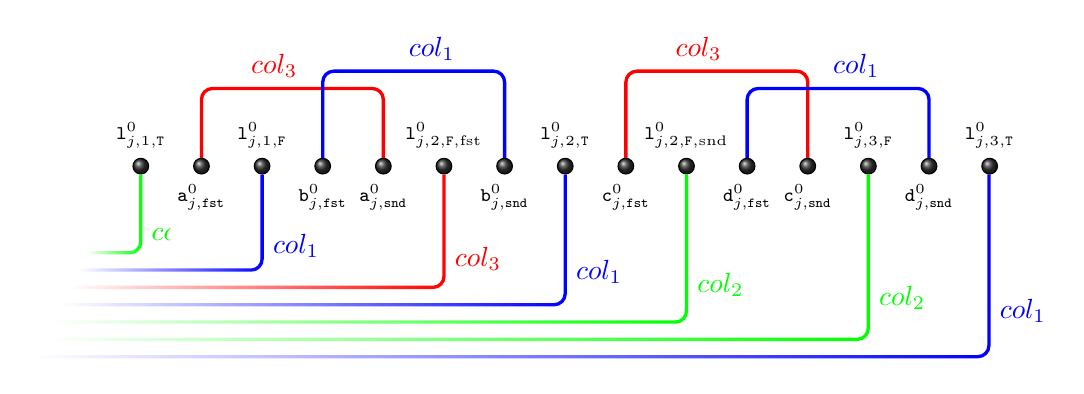
\begin{tikzpicture}
      [
      scale=.22,,,
      my vertex/.style={basic vertex,
      minimum size=1pt,
      inner sep=2pt,
      ball color=black!80},
      ]

      % vertices
      \foreach \i/\o/\l [evaluate=\i as \x using \i*3.5] in
      {
      1/above/\texttt{l}^0_{j,1,\TRUE},
      2/below/\texttt{a}^0_{j,\LEFT},
      3/above/\texttt{l}^0_{j,1,\FALSE},
      4/below/\texttt{b}^0_{j,\LEFT},
      5/below/\texttt{a}^0_{j,\RIGHT},
      6/above/\texttt{l}^0_{j,2,\FALSE,\FST},
      7/below/\texttt{b}^0_{j,\RIGHT},
      8/above/\texttt{l}^0_{j,2,\TRUE},
      9/below/\texttt{c}^0_{j,\LEFT},
      10/above/\texttt{l}^0_{j,2,\FALSE,\SND},
      11/below/\texttt{d}^0_{j,\LEFT},
      12/below/\texttt{c}^0_{j,\RIGHT},
      13/above/\texttt{l}^0_{j,3,\FALSE},
      14/below/\texttt{d}^0_{j,\RIGHT},
      15/above/\texttt{l}^0_{j,3,\TRUE}
      }
      {
      \node [my vertex,label=\o:{\scriptsize $\l$}] (V\i) at (\x,0) {};
      }

      % edges
      \path [edge,color=red] (V2.north) -- ++ (0,4) --
      ($(V5.north)+(0,4)$) node [pos=0.4,above] {$\COLOR_3$} -- (V5.north);

      \path [edge,color=blue] (V4.north) -- ++ (0,5) --
      ($(V7.north)+(0,5)$) node [pos=0.6,above] {$\COLOR_1$} -- (V7.north);

      \path [edge,color=red] (V9.north) -- ++ (0,5) --
      ($(V12.north)+(0,5)$) node [pos=0.4,above] {$\COLOR_3$} -- (V12.north);

      \path [edge,color=blue] (V11.north) -- ++ (0,4) --
      ($(V14.north)+(0,4)$) node [pos=0.6,above] {$\COLOR_1$} -- (V14.north);

      % incoming edges
      \draw [edge,color=green,path fading=west] (V1) -- node [pos=0.75,anchor=west] {$\COLOR_2$}
      ++(0,-5) -- +(-3,0) node {};

      \draw [edge,color=blue,path fading=west] (V3) -- node [pos=0.75,anchor=west] {$\COLOR_1$}
      ++(0,-6) -- +(-10.5,0) node {};

      \draw [edge,color=red,path fading=west] (V6)  -- node [pos=0.75,anchor=west] {$\COLOR_3$}
      ++(0,-7)  -- +(-21.5,0) node {};

      \draw [edge,color=blue,path fading=west] (V8)  -- node [pos=0.75,anchor=west] {$\COLOR_1$}
      ++(0,-8)  -- +(-29,0) node {};

      \draw [edge,color=green,path fading=west] (V10) -- node [pos=0.75,anchor=west] {$\COLOR_2$}
      ++(0,-9) -- +(-36.5,0) node {};

      \draw [edge,color=green,path fading=west] (V13) -- node [pos=0.75,anchor=west] {$\COLOR_2$}
      ++(0,-10) -- +(-47.5,0) node {};

      \draw [edge,color=blue,path fading=west] (V15) -- node [pos=0.75,anchor=west] {$\COLOR_1$}
      ++(0,-11) -- +(-55,0) node {};

      %\node [text width=2.5cm,anchor=west] at (-15.5,-8.5) {\scriptsize Towards the variable gadgets};

    \end{tikzpicture}
    \caption{%
    Clause gadget $\texttt{Cls}^{0}_{j}$ for clause $(\ell_{j,1} \vee \ell_{j,2} \vee \ell_{j,3})$
    in case the literals $\ell_{j,1}$, $\ell_{j,2}$ and $\ell_{j,3}$ evaluate to false, true and true,
    respectivelly, according to the satisfying assignment $f$.
    }% end caption
  \end{subfigure}

  \vspace{.5cm}

  \begin{subfigure}[b]{\textwidth}
    \centering
    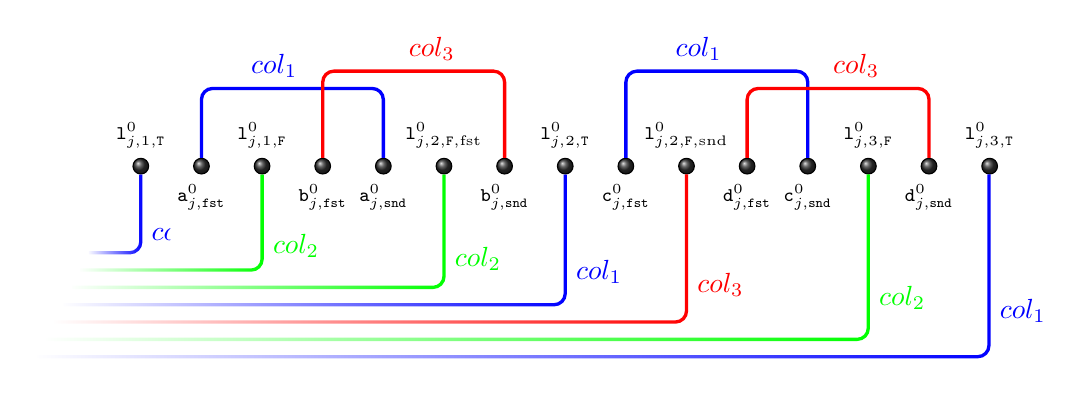
\begin{tikzpicture}
      [
      scale=.22,,,
      my vertex/.style={basic vertex,
      minimum size=1pt,
      inner sep=2pt,
      ball color=black!80},
      ]

      % vertices
      \foreach \i/\o/\l [evaluate=\i as \x using \i*3.5] in
      {
      1/above/\texttt{l}^0_{j,1,\TRUE},
      2/below/\texttt{a}^0_{j,\LEFT},
      3/above/\texttt{l}^0_{j,1,\FALSE},
      4/below/\texttt{b}^0_{j,\LEFT},
      5/below/\texttt{a}^0_{j,\RIGHT},
      6/above/\texttt{l}^0_{j,2,\FALSE,\FST},
      7/below/\texttt{b}^0_{j,\RIGHT},
      8/above/\texttt{l}^0_{j,2,\TRUE},
      9/below/\texttt{c}^0_{j,\LEFT},
      10/above/\texttt{l}^0_{j,2,\FALSE,\SND},
      11/below/\texttt{d}^0_{j,\LEFT},
      12/below/\texttt{c}^0_{j,\RIGHT},
      13/above/\texttt{l}^0_{j,3,\FALSE},
      14/below/\texttt{d}^0_{j,\RIGHT},
      15/above/\texttt{l}^0_{j,3,\TRUE}
      }
      {
      \node [my vertex,label=\o:{\scriptsize $\l$}] (V\i) at (\x,0) {};
      }

      % edges
      \path [edge,color=blue] (V2.north) -- ++ (0,4) --
      ($(V5.north)+(0,4)$) node [pos=0.4,above] {$\COLOR_1$} -- (V5.north);

      \path [edge,color=red] (V4.north) -- ++ (0,5) --
      ($(V7.north)+(0,5)$) node [pos=0.6,above] {$\COLOR_3$} -- (V7.north);

      \path [edge,color=blue] (V9.north) -- ++ (0,5) --
      ($(V12.north)+(0,5)$) node [pos=0.4,above] {$\COLOR_1$} -- (V12.north);

      \path [edge,color=red] (V11.north) -- ++ (0,4) --
      ($(V14.north)+(0,4)$) node [pos=0.6,above] {$\COLOR_3$} -- (V14.north);

      % incoming edges
      \draw [edge,color=blue,path fading=west] (V1) -- node [pos=0.75,anchor=west] {$\COLOR_1$}
      ++(0,-5) -- +(-3,0) node {};

      \draw [edge,color=green,path fading=west] (V3) -- node [pos=0.75,anchor=west] {$\COLOR_2$}
      ++(0,-6) -- +(-10.5,0) node {};

      \draw [edge,color=green,path fading=west] (V6)  -- node [pos=0.75,anchor=west] {$\COLOR_2$}
      ++(0,-7)  -- +(-21.5,0) node {};

      \draw [edge,color=blue,path fading=west] (V8)  -- node [pos=0.75,anchor=west] {$\COLOR_1$}
       ++(0,-8)  -- +(-29,0) node {};

      \draw [edge,color=red,path fading=west] (V10) -- node [pos=0.75,anchor=west] {$\COLOR_3$}
      ++(0,-9) -- +(-36.5,0) node {};

      \draw [edge,color=green,path fading=west] (V13) -- node [pos=0.75,anchor=west] {$\COLOR_2$}
      ++(0,-10) -- +(-47.5,0) node {};

      \draw [edge,color=blue,path fading=west] (V15) -- node [pos=0.75,anchor=west] {$\COLOR_1$}
      ++(0,-11) -- +(-55,0) node {};

      %\node [text width=2.5cm,anchor=west] at (-15.5,-8.5) {\scriptsize Towards the variable gadgets};

    \end{tikzpicture}
    \caption{%
    Clause gadget $\texttt{Cls}^{0}_{j}$ for clause $(\ell_{j,1} \vee \ell_{j,2} \vee \ell_{j,3})$
    in case the literals $\ell_{j,1}$, $\ell_{j,2}$ and $\ell_{j,3}$ evaluate to true, true and true,
    respectivelly, according to the satisfying assignment $f$.
    }% end caption
  \end{subfigure}
  \caption{The general caption.}
\end{figure}



\end{proof}


% Merging permutation
\section{Permutation coloring}
\label{section:Permutation coloring}

We are back to coloring permutations. We show how to transform
linear graph colorings to permutation colorings.
We need a new definition.
Let $G = (V, E)$ be a linear graph. For any two connected vertices
$v_i, v_j \in V$, $i < j$ or $j < i$,
we define
$$
\RANK(v_i, v_j) = \left|\left\{v_k \in V : \{v_i, v_k\} \in E \text{ and } k \leq j\right\}\right|.
$$
In other words, $\RANK(v_i, v_j) = k+1$ if there exist exactly $k$ vertices
$v_{i_1}, v_{i_2}, \dots, v_{i_k} \in N(v_i)$
with $\max \{i_1, i_2, \dots, i_k\} < j$.

\begin{proposition}
  \label{proposition:3-permutation coloring is NP-complete}
  \textsc{$3$-permutation coloring} is \NP-complete.
\end{proposition}

\begin{proof}
  We reduce from \textsc{$k$-Linear Graph Coloring} (Proposition~\ref{proposition:3-Linear Graph Coloring is NP-complete}).
  Let $(G^{0} \,|\, G^{1}, G^{2}, \dots, G^{k})$ be an arbitrary instance of \textsc{$k$-Linear Graph Coloring}.
  Write $G^{i} = (V^i, E^i)$,
  $n_i = |V^i|$ $m_i = |E^i|$ for $0 \leq i \leq k$.
  We show how to construct an instance
  $(\pi | \sigma_1, \sigma_2, \dots, \sigma_k)$ of
  \textsc{$k$-permutation coloring}.

  Define $N_i = 2n_i + 4m_i + 1$ for $0 \leq i \leq k$.
  We first associate the permutation $\pi$ to the linear graph $G^{0}$.
  Write $V^0 = \{v^0_i : 1 \leq i \leq n_0\}$ and
  $E^0 = \{e^0_i : 1 \leq i \leq m_0\}$.
  Define the permutations
  \begin{align*}
    \pi(V)
    &=
    \left(\bigoplus_{i=1}^{n_0} (d(v^0_i)+2) \; 1\right) [2m_0+2kN_0]
    \\
    \pi(E)
    &=
    \bigoplus_{j=1}^{m_0} 2 \; f^0(e^0_j) \; g^0(e^0_j) \; 1
    \\
    \pi(\text{Sep}_1)
    &=
    \left(\bigominus_{i=1}^{k} \mathbf{\nearrow}_{N_0}\right) [2n]
    \\
    \pi(\text{Sep}_2)
    &=
    \left(\bigominus_{i=1}^{k} \mathbf{\nearrow}_{N_0}\right) [2n+kN]
    \\
    \intertext{where $f : E^0 \to \mathbb{N}$ and $g : E^0 \to \mathbb{N}$
    are defined as follows}
    \forall e^0_j = (v^0_p, v^0_q) \in E_0,\quad f^0(e^0_j)
    &=
    2m_0 + 2kN_0 + \sum_{j=1}^{p-1}\left(2+d(v^0_j)\right) + \RANK\left(v^0_p, v^0_q\right)
    \\
    \forall e^0_j = (v^0_p, v^0_q) \in E_0,\quad g^0(e^0_j)
    &=
    2m_0 + 2kN_0 + \sum_{j=1}^{q-1}\left(2+d(v^0_j)\right) + \RANK\left(v^0_q, v^0_p\right)\text{.}
    \end{align*}

    In other words,
    $\pi(V)$ is the direct sum of $n_0$ decreasing permutations
    that are all order-isomorphic to $21$,
    $\pi(E)$ is the direct sum of $m_0$ permutations that are all
    order-isomorphic to $2341$ (since $2 < f(e^0_i) < g(e^0_i)$
    for $1 \leq i \leq m_0$), and
    both $\pi(\text{Sep}_1)$ and $\pi(\text{Sep}_2)$ are the skew sums
    of $k$ permutations that are all order isomorphic to $12 \dots k$.
    Finally, we obtain the target permutation $\pi$ by gathering the parts
    $\pi(V)$, $\pi(\text{Sep}_1)$, $\pi(E)$ and $\pi(\text{Sep}_2)$:
    $$
      \pi =
      \pi(V)   \;
      \pi(\text{Sep}_1) \;
      \pi(E)   \;
      \pi(\text{Sep}_2)\text{.}
    $$


  \begin{figure}[htbp!]
  \centering
  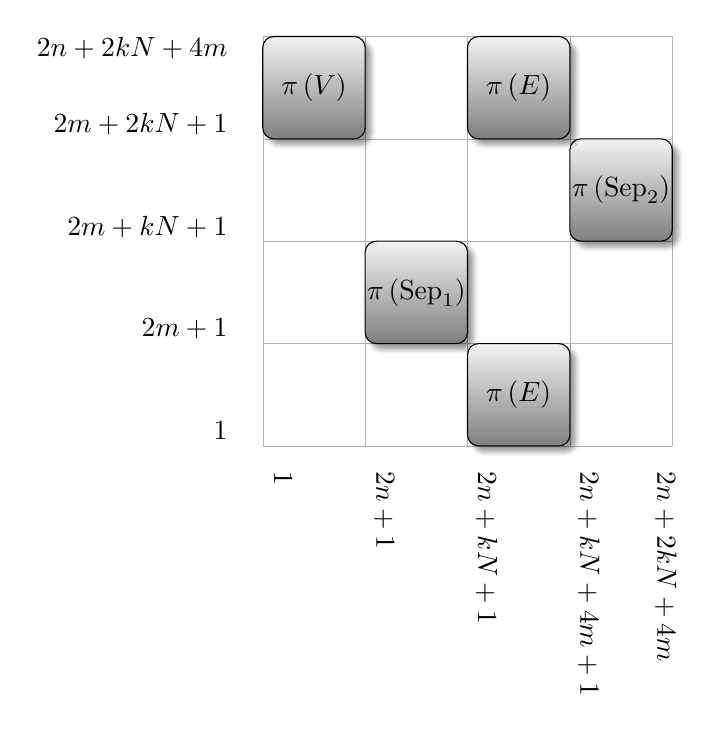
\begin{tikzpicture}
  [
    scale=.65,
    box/.style={
      shade,
      blur shadow={shadow blur steps=5,shadow blur extra rounding=1.3pt},
      top color=black!5,
      bottom color=black!50
    },
    gadget/.style={
      box,
      rounded corners
    },
    r/.style={
      box,
      draw,
      ultra thick,
    }
  ]
  \draw [help lines,step=2cm,black!30,fill=black!10] (0,0) grid (8,8);
  \draw [gadget] (0,6) rectangle ++(2,2);
  \node [] at (1,7) {$\pi\left(V\right)$};
  \draw [gadget] (2,2) rectangle ++(2,2);
  \node [] at (3,3) {$\pi\left(\text{Sep}_1\right)$};
  \draw [gadget] (4,0) rectangle ++(2,2);
  \node [] at (5,1) {$\pi\left(E\right)$};
  \draw [gadget] (6,4) rectangle ++(2,2);
  \node [] at (7,5) {$\pi\left(\text{Sep}_2\right)$};
  \draw [gadget] (4,6) rectangle ++(2,2);
  \node [] at (5,7) {$\pi\left(E\right)$};
    % labels
    % x-labels
    \node [label={[text depth=1.75ex,label distance=0.2cm,rotate=-90]right:{$1$}}] at (0,0) {};
    % \node [label={[text depth=1.75ex,label distance=0.2cm,rotate=-90]right:{$2n$}}] at (1.5,0) {};
    \node [label={[text depth=1.75ex,label distance=0.2cm,rotate=-90]right:{$2n+1$}}] at (2,0) {};
    % \node [label={[text depth=1.75ex,label distance=0.2cm,rotate=-90]right:{$2n+kN$}}] at (3.5,0) {};
    \node [label={[text depth=1.75ex,label distance=0.2cm,rotate=-90]right:{$2n+kN+1$}}] at (4,0) {};
    % \node [label={[text depth=1.75ex,label distance=0.2cm,rotate=-90]right:{$2n+kN+4m$}}] at (5.5,0) {};
    \node [label={[text depth=1.75ex,label distance=0.2cm,rotate=-90]right:{$2n+kN+4m+1$}}] at (6,0) {};
    \node [label={[text depth=1.75ex,label distance=0.2cm,rotate=-90]right:{$2n+2kN+4m$}}] at (7.5,0) {};
    % y-labels
    \node [label={[text depth=1.75ex,label distance=0.2cm]left:{$1$}}] at (0,0.1) {};
    % \node [label={[text depth=1.75ex,label distance=0.2cm]left:{$2m2$}}] at (0,1.6) {};
    \node [label={[text depth=1.75ex,label distance=0.2cm]left:{$2m+1$}}] at (0,2.1) {};
    % \node [label={[text depth=1.75ex,label distance=0.2cm]left:{$2m+kN$}}] at (0,3.6) {};
    \node [label={[text depth=1.75ex,label distance=0.2cm]left:{$2m+kN+1$}}] at (0,4.1) {};
    % \node [label={[text depth=1.75ex,label distance=0.2cm]left:{$2m+2kN$}}] at (0,5.6) {};
    \node [label={[text depth=1.75ex,label distance=0.2cm]left:{$2m+2kN+1$}}] at (0,6.1) {};
    \node [label={[text depth=1.75ex,label distance=0.2cm]left:{$2n+2kN+4m$}}] at (0,7.6) {};
  \end{tikzpicture}
  \caption{\label{fig:NP2:bird eye view pi}%
    Bird's-eye view of the permutation $\pi$.
  }% end caption
\end{figure}

  
\begin{figure}
  \centering
  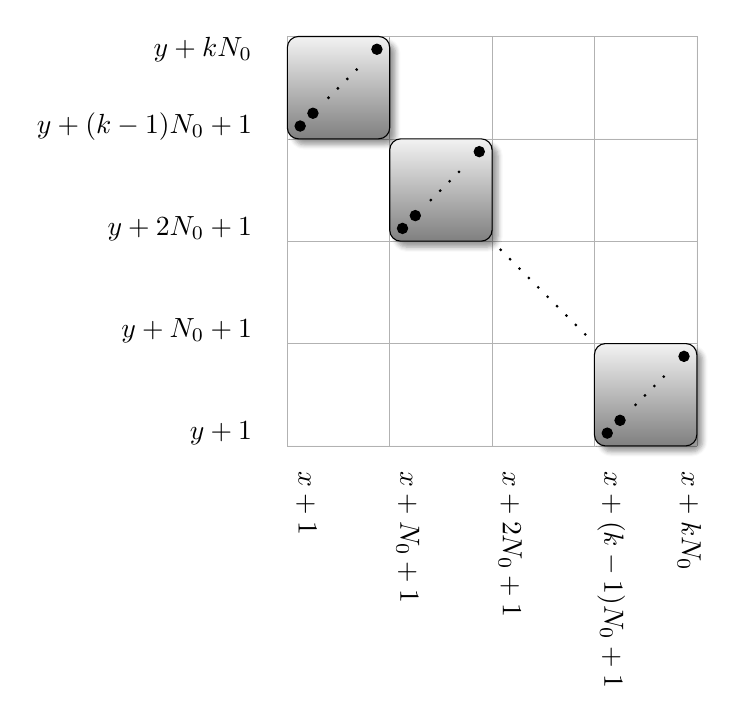
\begin{tikzpicture}
  [
    scale=.65,
    box/.style={
      shade,
      blur shadow={shadow blur steps=5,shadow blur extra rounding=1.3pt},
      top color=black!5,
      bottom color=black!50
    },
    monotone/.style={>=stealth',->,thick,shorten >=.5pt,shorten <=3pt},
  ]
    % separator gadgets
    % monotonic sequences
    \draw [help lines,step=2cm,black!30,fill=black!10] (0,0) grid (8,8);
    % I_1
    \draw [box,rounded corners] (0,6) rectangle ++(2,2);
    \foreach \x/\y in {0.25/6.25,0.5/6.5,1.75/7.75}
      \draw [fill=black] (\x,\y) circle (0.1);
    \draw [thick,loosely dotted,thick,shorten >=1pt,shorten <=1pt] (.75,6.75) -- (1.5,7.5);
    % I_2
    \draw [box,rounded corners] (2,4) rectangle ++(2,2);
    \foreach \x/\y in {2.25/4.25,2.5/4.5,3.75/5.75}
      \draw [fill=black] (\x,\y) circle (0.1);
    \draw [thick,loosely dotted,thick,shorten >=1pt,shorten <=1pt] (2.75,4.75) -- (3.5,5.5);
    % again and angain
    \draw [thick,loosely dotted,thick,shorten >=4pt,shorten <=4pt] (4,4) -- (6,2);
    % I_k
    \draw [box,rounded corners] (6,0) rectangle ++(2,2);
    \foreach \x/\y in {6.25/.25,6.5/.5,7.75/1.75}
      \draw [fill=black] (\x,\y) circle (0.1);
    \draw [thick,loosely dotted,thick,shorten >=1pt,shorten <=1pt] (6.75,.75) -- (7.5,1.5);
    % labels
    % x-labels
    \node [label={[text depth=1.75ex,label distance=0.2cm,rotate=-90]right:{$x+1$}}] at (0,0) {};
    % \node [label={[text depth=1.75ex,label distance=0.2cm,rotate=-90]right:{$x+N_0$}}] at (1.5,0) {};
    \node [label={[text depth=1.75ex,label distance=0.2cm,rotate=-90]right:{$x+N_0+1$}}] at (2,0) {};
    % \node [label={[text depth=1.75ex,label distance=0.2cm,rotate=-90]right:{$x+2N_0$}}] at (3.5,0) {};
    \node [label={[text depth=1.75ex,label distance=0.2cm,rotate=-90]right:{$x+2N_0+1$}}] at (4,0) {};
    % \node [label={[text depth=1.75ex,label distance=0.2cm,rotate=-90]right:{$x+(k-1)N_0$}}] at (5.5,0) {};
    \node [label={[text depth=1.75ex,label distance=0.2cm,rotate=-90]right:{$x+(k-1)N_0+1$}}] at (6,0) {};
    \node [label={[text depth=1.75ex,label distance=0.2cm,rotate=-90]right:{$x+kN_0$}}] at (7.5,0) {};
    % y-labels
    \node [label={[text depth=1.75ex,label distance=0.2cm]left:{$y+1$}}] at (0,0.1) {};
    % \node [label={[text depth=1.75ex,label distance=0.2cm]left:{$y+N_0$}}] at (0,1.6) {};
    \node [label={[text depth=1.75ex,label distance=0.2cm]left:{$y+N_0+1$}}] at (0,2.1) {};
    % \node [label={[text depth=1.75ex,label distance=0.2cm]left:{$y+2N_0$}}] at (0,3.6) {};
    \node [label={[text depth=1.75ex,label distance=0.2cm]left:{$y+2N_0+1$}}] at (0,4.1) {};
    % \node [label={[text depth=1.75ex,label distance=0.2cm]left:{$y+(k-1)N_0$}}] at (0,5.6) {};
    \node [label={[text depth=1.75ex,label distance=0.2cm]left:{$y+(k-1)N_0+1$}}] at (0,6.1) {};
    \node [label={[text depth=1.75ex,label distance=0.2cm]left:{$y+kN_0$}}] at (0,7.6) {};
  \end{tikzpicture}
  \caption{\label{fig:NP2:separators}%
    Schematic representation of $\pi(\text{Sep}_1)$ and $\pi(\text{Sep}_2)$,
    where the offsetis $O=2n$ for
    $\pi(\text{Sep}_1)$ and $O=2n+kN$ for $\pi(\text{Sep}_2)$.
  }% end caption
\end{figure}

  \begin{figure}
  \centering
  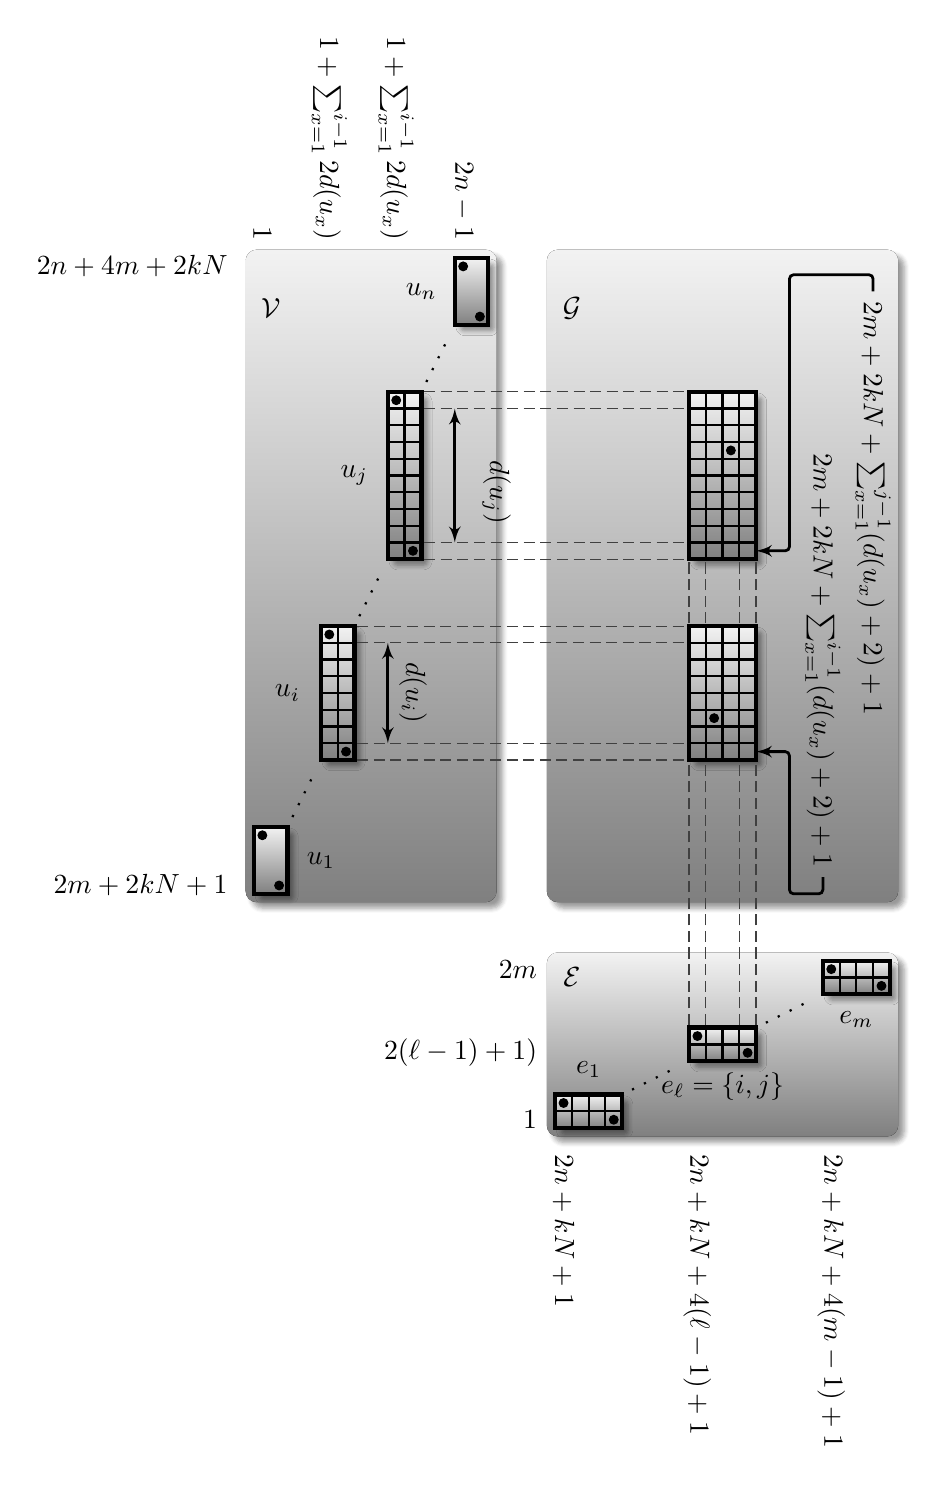
\begin{tikzpicture}
  [
    scale=.425,
    box/.style={
      shade,
      blur shadow={shadow blur steps=5,shadow blur extra rounding=1.3pt},
      top color=black!5,
      bottom color=black!50
    },
    gadget/.style={
      box,
      rounded corners
    },
    r/.style={
      box,
      draw,
      ultra thick,
    }
  ]
    % V gadget
    \fill [gadget] (-0.25,9.75) rectangle (7.25,29.25);
    \node at (0.5,27.5) {$\mathcal{V}$};
    % vertex 1
    \path [r] (0,10) -- ++(1,0) -- ++(0,2) -- ++(-1,0) -- cycle;
    \foreach \x/\y in {0.25/11.75,0.75/10.25}
      \draw [fill=black] (\x,\y) circle (0.13);
    \node at (2,11) {$u_1$};
    % again and again
    \draw [thick,loosely dotted,thick,shorten >=4pt,shorten <=4pt] (1,12) -- (2,14);
    % vertex i
    \path [r] (2,14) -- ++(1,0) -- ++(0,4) -- ++(-1,0) -- cycle;
    \draw [thick,step=0.5cm] (2,14) grid (3,18);
    \path [draw,ultra thick] (2,14) -- ++(1,0) -- ++(0,4) -- ++(-1,0) -- cycle;
    \foreach \x/\y in {2.25/17.75,2.75/14.25}
      \draw [fill=black] (\x,\y) circle (0.13);
    \node at (1,16) {$u_i$};
    % again and again
    \draw [thick,loosely dotted,thick,shorten >=4pt,shorten <=4pt] (3,18) -- (4,20);
    % vertex j
    \path [r] (4,20) -- ++(1,0) -- ++(0,5) -- ++(-1,0) -- cycle;
    \draw [thick,step=0.5cm] (4,20) grid (5,25);
    \path [draw,ultra thick] (4,20) -- ++(1,0) -- ++(0,5) -- ++(-1,0) -- cycle;
    \foreach \x/\y in {4.25/24.75,4.75/20.25}
      \draw [fill=black] (\x,\y) circle (0.13);
    \node at (3,22.5) {$u_j$};
    % again and again
    \draw [thick,loosely dotted,thick,shorten >=4pt,shorten <=4pt] (5,25) -- (6,27);
    % vertex n
    \path [r] (6,27) -- ++(1,0) -- ++(0,2) -- ++(-1,0) -- cycle;
    \foreach \x/\y in {6.25/28.75,6.75/27.25}
      \draw [fill=black] (\x,\y) circle (0.13);
    \node at (5,28) {$u_n$};

    % E gadget
    \fill [gadget] (8.75,2.75) rectangle (19.25,8.25);
    \node at (9.5,7.5) {$\mathcal{E}$};
    % first edge
    \path [r] (9,3) -- ++(2,0) -- ++(0,1) -- ++(-2,0) -- cycle;
    \draw [thick,step=0.5cm] (9,3) grid (11,4);
    \path [draw,ultra thick] (9,3) -- ++(2,0) -- ++(0,1) -- ++(-2,0) -- cycle;
    \foreach \x/\y in {9.25/3.75,10.75/3.25}
      \draw [fill=black] (\x,\y) circle (0.13);
    \node at (10,4.75) {$e_1$};
    % again and again
    \draw [thick,loosely dotted,thick,shorten >=4pt,shorten <=4pt] (11,4) -- (13,5);
    % edge (i,j))
    \path [r] (13,5) -- ++(2,0) -- ++(0,1) -- ++(-2,0) -- cycle;
    \draw [thick,step=0.5cm] (13,5) grid (15,6);
    \path [draw,ultra thick] (13,5) -- ++(2,0) -- ++(0,1) -- ++(-2,0) -- cycle;
    \foreach \x/\y in {13.25/5.75,14.75/5.25}
      \draw [fill=black] (\x,\y) circle (0.13);
    \node at (14,4.25) {$e_\ell = \{i,j\}$};
    % again and again
    \draw [thick,loosely dotted,thick,shorten >=4pt,shorten <=4pt] (15,6) -- (17,7);
    % last edge
    \path [r] (17,7) -- ++(2,0) -- ++(0,1) -- ++(-2,0) -- cycle;
    \draw [thick,step=0.5cm] (17,7) grid (19,8);
    \path [draw,ultra thick] (17,7) -- ++(2,0) -- ++(0,1) -- ++(-2,0) -- cycle;
    \foreach \x/\y in {17.25/7.75,18.75/7.25}
      \draw [fill=black] (\x,\y) circle (0.13);
    \node at (18,6.25) {$e_m$};

    % Connection gadget
    \fill [gadget] (8.75,9.75) rectangle (19.25,29.25);
    \node at (9.5,27.5) {$\mathcal{G}$};
    \fill [r] (13-0.001,14-0.001) rectangle (15,18);
    \draw [thick,step=0.5cm,black] (13-0.001,14-0.001) grid (15,18);
    \draw [fill=black] (13.75,15.25) circle (0.13);
    \fill [r] (13-0.001,20-0.001) rectangle (15,25);
    \draw [thick,step=0.5cm,black] (13-0.001,20-0.001) grid (15,25);
    \draw [fill=black] (14.25,23.25) circle (0.13);

    %  alignments
    % vertical
    \draw [black!75,dash pattern={on 4pt off 2pt},shorten >=1pt,shorten <=1pt] (13,6) -- (13,14);
    \draw [black!75,dash pattern={on 4pt off 2pt},shorten >=1pt,shorten <=1pt] (13,18) -- (13,20);
    \draw [black!75,dash pattern={on 4pt off 2pt},shorten >=1pt,shorten <=1pt] (15,6) -- (15,14);
    \draw [black!75,dash pattern={on 4pt off 2pt},shorten >=1pt,shorten <=1pt] (15,18) -- (15,20);
    %
    \draw [black!75,dash pattern={on 4pt off 2pt},shorten >=1pt,shorten <=1pt] (13.5,6) -- (13.5,14);
    \draw [black!75,dash pattern={on 4pt off 2pt},shorten >=1pt,shorten <=1pt] (13.5,18) -- (13.5,20);
    \draw [black!75,dash pattern={on 4pt off 2pt},shorten >=1pt,shorten <=1pt] (14.5,6) -- (14.5,14);
    \draw [black!75,dash pattern={on 4pt off 2pt},shorten >=1pt,shorten <=1pt] (14.5,18) -- (14.5,20);
    % horizontal
    \draw [black!75,dash pattern={on 4pt off 2pt},shorten >=1pt,shorten <=1pt] (3,14) -- (13,14);
    \draw [black!75,dash pattern={on 4pt off 2pt},shorten >=1pt,shorten <=1pt] (3,14.5) -- (13,14.5);
    \draw [black!75,dash pattern={on 4pt off 2pt},shorten >=1pt,shorten <=1pt] (3,17.5) -- (13,17.5);
    \draw [black!75,dash pattern={on 4pt off 2pt},shorten >=1pt,shorten <=1pt] (3,18) -- (13,18);
    \draw [black,line width=1pt,<->,>=latex'] (4,14.5) -- (4,17.5);
    \node [rotate=-90] at (4.75,16) {$d(u_i)$};
    \draw [black!75,dash pattern={on 4pt off 2pt},shorten >=1pt,shorten <=1pt] (5,20) -- (13,20);
    \draw [black!75,dash pattern={on 4pt off 2pt},shorten >=1pt,shorten <=1pt] (5,20.5) -- (13,20.5);
    \draw [black!75,dash pattern={on 4pt off 2pt},shorten >=1pt,shorten <=1pt] (5,24.5) -- (13,24.5);
    \draw [black!75,dash pattern={on 4pt off 2pt},shorten >=1pt,shorten <=1pt] (5,25) -- (13,25);
    \draw [black,line width=1pt,<->,>=latex'] (6,20.5) -- (6,24.5);
    \node [rotate=-90] at (7.25,22) {$d(u_j)$};

    % labels
    % vertex gadget
    % x-labels
    \node [anchor=east,rotate=-90] at (0.25,29.25) {$1$};
    \node [anchor=east,rotate=-90] at (2.25,29.25) {$1 + \sum_{x=1}^{i-1}2d(u_x)$};
    \node [anchor=east,rotate=-90] at (4.25,29.25) {$1 + \sum_{x=1}^{i-1}2d(u_x)$};
    \node [anchor=east,rotate=-90] at (6.25,29.25) {$2n-1$};
    % y-labels
    \node [anchor=east] at (-0.5,10.25) {$2m+2kN+1$};
    \node [anchor=east] at (-0.5,28.75) {$2n+4m+2kN$};
    % edge gadget
    % x-labels
    \node [rotate=-90,anchor=west] at (9.25,2.5) {$2n+kN+1$};
    \node [rotate=-90,anchor=west] at (13.25,2.5) {$2n+kN+4(\ell-1)+1$};
    \node [rotate=-90,anchor=west] at (17.25,2.5) {$2n+kN+4(m-1)+1$};
    % y-labels
    \node [anchor=east] at (8.75,3.25) {$1$};
    \node [anchor=east] at (8.75,5.25) {$2(\ell-1)+1)$};
    \node [anchor=east] at (8.75,7.75) {$2m$};
    % connection labels
    % y-labels
    \node [anchor=east,rotate=-90] at (17,10.5) {$2m+2kN+\sum_{x=1}^{i-1}(d(u_x)+2)+1$};
    \draw [black,line width=1pt,->,>=latex',rounded corners=1.5pt]
      (17,10.5) -- (17,10) -- (16,10) -- (16,14.25) -- (15,14.25);
    \node [anchor=west,rotate=-90] at (18.5,28) {$2m+2kN+\sum_{x=1}^{j-1}(d(u_x)+2)+1$};
    \draw [black,line width=1pt,->,>=latex',rounded corners=1.5pt]
      (18.5,28) -- (18.5,28.5) -- (16,28.5) -- (16,20.25) -- (15,20.25);
  \end{tikzpicture}
  \caption{\label{fig:NP2:connection zoom}%
  $\RANK(u_i, u_j) = 2$ and $\RANK(u_j, u_i) = 6 = d(u_j)$.
  }% end caption
\end{figure}


  A simplified representation of the permutation $\pi$ is given in
  Figure~\ref{fig:NP2:bird eye view pi}.
  A schematic representation of $\pi(\text{Sep}_1)$ and $\pi(\text{Sep}_2)$
  is given in Figure~\ref{fig:NP2:separators}, where the offset is $O=2n$ for
  $\pi(\text{Sep}_1)$ and $O=2n+kN$ for $\pi(\text{Sep}_2)$.
  A zoom of $\pi(E)$ is given in Figure~\ref{fig:NP2:connection zoom}.

  For example, referring Figure~\ref{fig:3-Linear-Graph Coloring} ($k=3$), we
  obtain from the linear graph $G^0$:
  $N_0 = 26 + 44 + 1 = 71$, $2m0+2kN_0= 22 + 426 = 448$, and hence
  $\pi(V) = \left(3 1 \oplus 3 1 \oplus 4 1 \oplus 4 1 \oplus 4 1 \oplus
  4 1 \oplus 4 1 \oplus 4 1 \oplus 4 1 \oplus 3 1 \oplus 3 1 \oplus 4 1 \oplus 3 1\right) [448]$,
  $\pi(E) = 2\;449\;479\;1 \oplus \dots$

  We now turn to associating the permutation $\sigma_i$, $1 \leq i \leq k$,
  to the linear graph $G^i = (V^i, E^i)$.
  The construction, as a whole, follows the same line as of $\pi$,
  the main difference being the \emph{separators}
  $\sigma_i\left(\text{Sep}_1\right)$ and
  $\sigma_i\left(\text{Sep}_2\right)$ that are both simplified.
  Define
  \begin{align*}
    \sigma_i(V)
    &=
    \left(\bigoplus_{j=1}^{n_i} (d(v^i_j)+2) \; 1\right) [2m_i+2N_i]
    \\
    \sigma_i(E)
    &=
    \bigoplus_{j=1}^{m_i} 2 \; f^i(e^0_j) \; g^i(e^0_j) \; 1
    \\
    \sigma_i\left(\text{Sep}_1\right)
    &=
    \mathbf{\nearrow}_{N_0} [2n_i]
    \\
    \sigma_i\left(\text{Sep}_2\right)
    &=
    \mathbf{\nearrow}_{N_0} [2n_i+N]
    \\
    \intertext{where $f^i : E^i \to \mathbb{N}$ and $g^i : E^i \to \mathbb{N}$
    are defined as follows}
    \forall e^i_j = (v^i_p, v^i_q) \in E_i,\quad f^i(e^0_j)
    &=
    2m_0 + 2kN_0 + \sum_{j=1}^{p-1}\left(2+d(v^0_j)\right) + \RANK\left(v^0_p, v^0_q\right)
    \\
    \forall e^i_j = (v^i_p, v^0_q) \in E_i,\quad g^i(e^0_j)
    &=
    2m_0 + 2kN_0 + \sum_{j=1}^{q-1}\left(2+d(v^0_j)\right) + \RANK\left(v^0_q, v^0_p\right)\text{.}
    \end{align*}
  %
  %   \intertext{where (assuming edge $e_{i,\ell} = (u_i, u_j)$)}
  %   x^1_{i,\ell}
  %   &=
  %   2m + 2kN + \sum_{\ell'=1}^{i-1}\left(2+d(u_{\ell'})\right) + \RANK\left(u_i, u_j\right)
  %   \\
  %   x^2_{i,\ell}
  %   &=
  %   2m + 2kN + \sum_{\ell'=1}^{j-1}\left(2+d(u_{\ell'})\right) + \RANK\left(u_j, u_i\right),
  %   \\
  %   \intertext{and set}
  %   \sigma_i
  %   &=
  %   \sigma_i(V)   \;
  %   \sigma_i\left(\text{Sep}_1\right) \;
  %   \sigma_i\left(E\right)   \;
  %   \sigma_i\left(\text{Sep}_1\right)\text{.}
  % \end{align*}

  \begin{figure}[htbp!]
  \centering
  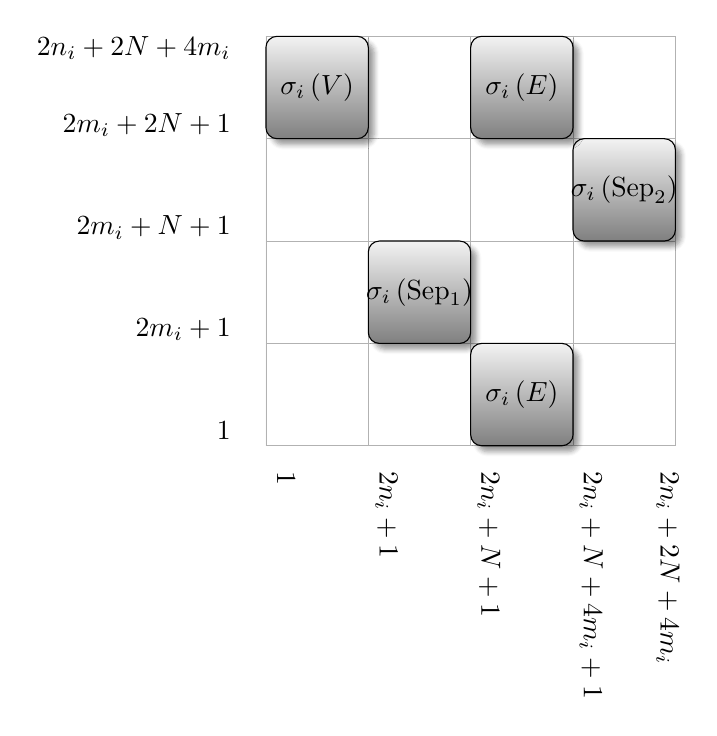
\begin{tikzpicture}
  [
    scale=.65,
    box/.style={
      shade,
      blur shadow={shadow blur steps=5,shadow blur extra rounding=1.3pt},
      top color=black!5,
      bottom color=black!50
    },
    gadget/.style={
      box,
      rounded corners
    },
    r/.style={
      box,
      draw,
      ultra thick,
    }
  ]
    \draw [help lines,step=2cm,black!30,fill=black!10] (0,0) grid (8,8);
    \draw [gadget] (0,6) rectangle ++(2,2);
    \node [] at (1,7) {$\sigma_i\left(V\right)$};
    \draw [gadget] (2,2) rectangle ++(2,2);
    \node [] at (3,3) {$\sigma_i\left(\text{Sep}_1\right)$};
    \draw [gadget] (4,0) rectangle ++(2,2);
    \node [] at (5,1) {$\sigma_i\left(E\right)$};
    \draw [gadget] (6,4) rectangle ++(2,2);
    \node [] at (7,5) {$\sigma_i\left(\text{Sep}_2\right)$};
    \draw [gadget] (4,6) rectangle ++(2,2);
    \node [] at (5,7) {$\sigma_i\left(E\right)$};
    % labels
    % x-labels
    \node [label={[text depth=1.75ex,label distance=0.2cm,rotate=-90]right:{$1$}}] at (0,0) {};
    % \node [label={[text depth=1.75ex,label distance=0.2cm,rotate=-90]right:{$2n$}}] at (1.5,0) {};
    \node [label={[text depth=1.75ex,label distance=0.2cm,rotate=-90]right:{$2n_i+1$}}] at (2,0) {};
    % \node [label={[text depth=1.75ex,label distance=0.2cm,rotate=-90]right:{$2n+kN$}}] at (3.5,0) {};
    \node [label={[text depth=1.75ex,label distance=0.2cm,rotate=-90]right:{$2n_i+N+1$}}] at (4,0) {};
    % \node [label={[text depth=1.75ex,label distance=0.2cm,rotate=-90]right:{$2n+kN+4m$}}] at (5.5,0) {};
    \node [label={[text depth=1.75ex,label distance=0.2cm,rotate=-90]right:{$2n_i+N+4m_i+1$}}] at (6,0) {};
    \node [label={[text depth=1.75ex,label distance=0.2cm,rotate=-90]right:{$2n_i+2N+4m_i$}}] at (7.5,0) {};
    % y-labels
    \node [label={[text depth=1.75ex,label distance=0.2cm]left:{$1$}}] at (0,0.1) {};
    % \node [label={[text depth=1.75ex,label distance=0.2cm]left:{$2m2$}}] at (0,1.6) {};
    \node [label={[text depth=1.75ex,label distance=0.2cm]left:{$2m_i+1$}}] at (0,2.1) {};
    % \node [label={[text depth=1.75ex,label distance=0.2cm]left:{$2m+kN$}}] at (0,3.6) {};
    \node [label={[text depth=1.75ex,label distance=0.2cm]left:{$2m_i+N+1$}}] at (0,4.1) {};
    % \node [label={[text depth=1.75ex,label distance=0.2cm]left:{$2m+2kN$}}] at (0,5.6) {};
    \node [label={[text depth=1.75ex,label distance=0.2cm]left:{$2m_i+2N+1$}}] at (0,6.1) {};
    \node [label={[text depth=1.75ex,label distance=0.2cm]left:{$2n_i+2N+4m_i$}}] at (0,7.6) {};
  \end{tikzpicture}
  \caption{\label{fig:NP2:bird eye view sigma_i}%
    Bird's-eye view of the permutation $\sigma_i$.
  }% end caption
\end{figure}


  A schematic representation of the permutation $\sigma_i$ is given in
  Figure~\ref{fig:NP2:bird eye view sigma_i}.

  Clearly our construction can be carried on in polynomial time.
  Indeed, we have
  $|\pi| = 2n + 4m + 2kN = 2n + 4m + 2k(2n+4m+1)$
  and
  $|\sigma_i| = 2n_i + 4m_i + 2N = 2n_i + 4m_i + 2(2n+4m+1)$,
  $1 \leq i \leq k$.
  We claim that the linear graph $G^0$ is
  $(G^1, G^2, \dots, G^k)$-colorable
  if and only if the permutation
  $\pi$ is $(\sigma_1, \sigma_2, \dots, \sigma_k)$-colorable.

  Suppose first that $G^0$ is $(G^1, G^2, \dots, G^k)$-colorable.
  Therefore, there exists a $k$-coloring such that
  every connected component of $G^0$ is monochromatic and,
  for every $1 \leq i \leq k$, colour $i$ induces a linear graph that is
  isomorphic to $G^i$.
  For every $1 \leq i \leq k$,
  let $v_{i_1}< v_{i_2} < \dots < v_{i_{n_i}}$ be the vertices of $G^0$ with color $i$.
  Let us now define a $k$-colouring $\varphi: [|\pi|] \to [k]$ of $\pi$ as follows.
  \begin{itemize}
    \item \textbf{Gadget $\pi(V)$}.
    For every $1 \leq j \leq n_i$,
    $\varphi(2i_j-2) = \varphi(2i_j-1) = i$
    \item \textbf{Gadget $\pi(\text{Sep}_1)$}.
    Colour the $i$-th increasing sequence $\nearrow_{N_0}$ with colour $i$.
    More formally,
    for every $2n + N_0(i-1) + 1 \leq j \leq 2n + iN_0$,
    $\varphi(j) = i$.
    \item \textbf{Gadget $\pi(E)$}.
    Let $e_{i_1} < e_{i_2} < \ldots < ae{i_{m_i}}$ be the edges of $G^0$ that connect
    vertices coloured with colour $i$.
    For every $1 \leq j \leq m_i$,
    $\varphi(2n + kN_0 + 4(i_j-1) + 1) = \varphi(2n + kN_0 + 4(i_j-1) + 2) =
    \varphi(2n + kN_0 + 4(i_j-1) + 3) = \varphi(2n + kN_0 + 4(i_j-1) + 4) = i$.
    \item \textbf{Gadget $\pi(\text{Sep}_2)$}.
    Colour the $i$-th increasing sequence $\nearrow_{N_0}$ with colour $i$.
    More formally,
    for every $2n + kN_0 + 4m + N_0(i-1) + 1 \leq j \leq 2n + kN_0 + 4m + iN_0$,
    $\varphi(j) = i$.
  \end{itemize}
  The reader is invited to check that, for every $1 \leq i \leq k$,
  the $i$-coloured pattern of $\pi$ is order-isomorphic to $\sigma_i$.

  Conversely, suppose that $\pi$ is $(\sigma_1, \sigma_2, \dots, \sigma_k)$-colorable.
  Therefore, there exists a $k$-coloring $\varphi: [2n_0 + 4m_0 + 2kN_0] \to [k]$
  such that, for every $1 \leq i \leq k$,
  the $i$-coloured pattern of $\pi$ is order-isomorphic to $\sigma_i$.
  Let us focus on $\sigma_i$ for some $1 \leq i \leq k$.
  Recall that
  $\sigma_i =
  \sigma_i(V)   \;
  \sigma_i\left(\text{Sep}_1\right) \;
  \sigma_i\left(E\right)   \;
  \sigma_i\left(\text{Sep}_1\right)$,
  where both
  $\sigma_i\left(\text{Sep}_1\right)$ and $\sigma_i\left(\text{Sep}_2\right)$
  are increasing sequence of length $N_0$.
  We now oberve that
  $N_0 > |\pi(V)| + |\pi(E)|$.
  Then it follows that
  (i) at least one element of $\pi(\text{Sep}_1)$ is coloured with
  colour $i$,
  and
  (ii) at least of element of $\pi(\text{Sep}_2)$ is coloured with
  colour $i$.
  But
  $\pi(\text{Sep}_1) \; \pi(\text{Sep}_2)$ and
  $\sigma_i\left(\text{Sep}_1\right) \; \sigma_i\left(\text{Sep}_2\right)$
  are both order-isomorphic to
  $\left(\bigominus_{\ell=1}^{k} \nearrow_N\right) \oplus \left(\bigominus_{\ell=1}^{k} \nearrow_N\right)$,
  and hence
  (i) $N$ vertices of $\pi(\text{Sep}_1)$ are coloured with
  colour $i$,
  and
  (ii) $N$ vertices of $\pi(\text{Sep}_1)$ are coloured with
  colour $i$.
  Therefore,
  (i) $|\sigma_i(V)| = 2n_i$ elements of
  $\pi(V)$ are coloured with colour $i$ and the induced
  $i$-coloured pattern is order-isomorphic to $\sigma_i(V)$,
  and
  (ii) $|\sigma_i\left(E\right)| = 4m_i$ elements of
  $\pi(E)$ are coloured with colour $i$ and the induced
  $i$-coloured pattern is order-isomorphic to $\sigma_i\left(E\right)$.
  But $\pi(V)$ is order-isomorphic to $\bigoplus_{\ell=1}^{n} 21$
  and
  $\sigma_i(V)$ is order-isomorphic to $\bigoplus_{\ell=1}^{n_i} 21$.
  Therefore, $n_i$ patterns $21$ are coloured with colour $i$ thereby identifying
  $n_i$ vertices of $G$.
  Finally,
  combining
  $\pi(E) = \bigoplus_{\ell=1}^{m} 2 \; x_\ell^1 \; x_\ell^2 \; 1$ and
  $\sigma_i\left(E\right) = \bigoplus_{\ell=1}^{m_i} 2 \; x_{i,\ell^1} \; x_{i,\ell^2} \; 1$,
  together with the fact that $x_{i,\ell^1}$ and $x_{i,\ell^2}$ have to be sandwiched in
  $i$-coloured pattern $21$ of $\pi(V)$,
  we conclude that $m_i$ consecutive patterns $2 \; x_{i,\ell^1} \; x_{i,\ell^2} \; 1$
  of $\pi(E)$ are coloured with colour $i$.
  Hence, \todo{Ok I'm lazy (or tired), this is not formal!}referring to
  Figure~\ref{fig:NP2:connection zoom} and considering every $1 \leq i \leq k$,
  we conclude that $G$ can be splitted by linear graphs $H_1, H_2, \ldots, H_k$.
  \qed
\end{proof}

\begin{corollary}
  \label{corollary:5-permutation coloring is NP-complete}
  \textsc{$3$-permutation coloring} is \NPC.
\end{corollary}

\begin{proof}
  Combine Proposition~\ref{proposition:3-Linear Graph Coloring}
  with Proposition~\ref{proposition:k-linear-graph coloring < k-permutation coloring}.
  \qed
\end{proof}

It is worth noticing that, according to
Proposition~\ref{proposition:k-linear-graph coloring < k-permutation coloring},
any improvement on Proposition~\ref{proposition:5-linear-graph coloring is NP-complete}
would immediately propagate to \textsc{$k$-permutation coloring}.


% Merging monotonic patterns
=======
% Matching coloring
\subsubsection{Merging matchings}
\label{section:Merging matchings}

This section is devoted to proving that the
\textsc{$3$-Merge Matchings} is \NP-complete.

\begin{proposition}
  \label{proposition:3-merge matching is NP-complete}
  \textsc{$3$-Merge Matching} is \NP-complete.
\end{proposition}

\begin{proof}
  We reduce from the \textsc{$3$-Sat} problem, which is known to
  \NP-complete \cite{DBLP:conf/coco/Karp72}.
  Let $\phi = c_1 \wedge c_2 \wedge \cdots \wedge c_m$ be a CNF formula
  defined over the boolean variables $X =\{x_1, x_2, \dots, x_n\}$.
  For every variable $x_{i} \in X$,
  we let $\OCCURRENCE_1(x_{i})$ (resp. $\OCCURRENCE_2(x_{i})$ and $\OCCURRENCE_3(x_{i})$)
  stand for the number of occurrences of the variable $x_{i}$ as the first (resp. second and third)
  literal of a clause.
  Furthermore, we let $\OCCURRENCE(x_{i})$ stand for
  $\OCCURRENCE_1(x_{i}) + 2\,\OCCURRENCE_2(x_{i}) + \OCCURRENCE_3(x_{i})$.
  For any clause $c$, we let $c[i]$ stand for
  $i$-th literal of $c$.

  We define an instance of the \textsc{$3$-matching Coloring} problem by defining a
  target matching $\mathcal{M}{0} = (V^{0}, E^{0})$
  and three matchings
  $\mathcal{M}{1} = (V^{1}, E^{1})$, $\mathcal{M}{2} = (V^{2}, E^{2})$ and $\mathcal{M}{3} = (V^{3}, E^{3})$.
  All matchings $\mathcal{M}{0}$, $\mathcal{M}{1}$, $\mathcal{M}{2}$ and $\mathcal{M}{3}$ are actually composed
  of independent edges so that any connected component is composed of two vertices only.
  The general idea of the reduction is as follows:
  the target matching $\mathcal{M}{0}$ encodes the whole instance
  and $\mathcal{M}{1}$ encodes an assignment of the variable that satisfies all clauses of $\phi$;
  both $\mathcal{M}{2}$ and $\mathcal{M}{3}$ act as garbage collectors by focusing of those edges of $\mathcal{M}{0}$
  that are not part of the satisfying assignment or are structure edges.

  Set $N=m^2$.
  We have divided the presentation of the matchings $\mathcal{M}{0}, \mathcal{M}{1}, \mathcal{M}{2}$ and $\mathcal{M}{3}$.

  % matching \mathcal{M}0
  \medskip
  \textbf{Defining the target matching $\mathcal{M}{0} = (V^{0}, E^{0})$}
  \medskip

  % \begin{mdframed}
    Define
    \begin{alignat*} {2}
      V^{0} &= \texttt{Var}^{0} \cup \texttt{Cls}^{0}
      &\quad&\text{with $\texttt{Var}^{0} < \texttt{Cls}^{0}$,}
      \\
      \texttt{Var}^{0} &= \bigcup_{i=1}^{n} \texttt{Var}^{0}_{i}
      &&\text{with $\texttt{Var}^{0}_1 < \texttt{Var}^{0}_2 < \cdots < \texttt{Var}^{0}_n$,}
      \\
      \texttt{Cls}^{0} &= \bigcup_{j=1}^{m} \texttt{Cls}^{0}_{j}
      &&\text{with $\texttt{Cls}^{0}_1 < \texttt{Cls}^{0}_2 < \cdots < \texttt{Cls}^{0}_m$.}
    \end{alignat*}

    Let us first define the vertices of $\texttt{Var}^{0}$ that correspond
    to the variables $X$.
    Quite naturally, the vertices of $\texttt{Var}^{0}_{i}$, $1 \leq i \leq n$,
    are associated to the boolean variable $x_{i} \in X$.
    For $1 \leq i \leq n$, define
    \begin{alignat*}{2}
      \texttt{Var}^{0}_{i} &=
      &&
      \texttt{T}^{0}_{i,\LEFT} \cup \texttt{T}^{0}_{i,\RIGHT} \cup
      \texttt{F}^{0}_{i,\LEFT} \cup \texttt{F}^{0}_{i,\RIGHT} \cup
      \texttt{Y}^{0}_{i,\LEFT} \cup \texttt{Y}^{0}_{i,\RIGHT} \cup
      \texttt{X}^{0}_{i} \cup \neg\texttt{X}^{0}_{i}
      \\
      \intertext{
      with $$\texttt{T}^{0}_{i,\LEFT} <
      \texttt{Y}^{0}_{i,\LEFT} <
      \texttt{X}^{0}_{i} <
      \texttt{F}^{0}_{i,\LEFT} <
      \texttt{T}^{0}_{i,\RIGHT} <
      \neg\texttt{X}^{0}_{i} <
      \texttt{Y}^{0}_{i,\RIGHT} <
      \texttt{F}^{0}_{i,\RIGHT},$$
      and}
      \texttt{T}^{0}_{i,\LEFT}
      &=
      &&\{\texttt{t}^{0}_{i,j,\LEFT} : 1 \leq j \leq N\}
      \\
      \texttt{Y}^{0}_{i,\LEFT}
      &=
      &&\{\texttt{y}^{0}_{i,j,\LEFT} : 1 \leq j \leq N\}
      \\
      \texttt{X}^{0}_{i}
      &=
      &&\texttt{X}^{0}_{i,1} \cup \texttt{X}^{0}_{i,2} \cup \texttt{X}^{0}_{i,3}
      \\
      \texttt{X}^{0}_{i,1}
      &=
      &&\{\texttt{x}^{0}_{i,1,j} :
      \text{$c_{j}[1] = x_{i}$ or $c_{j}[1] = \overline{x_{i}}$}\}
      \\
      \texttt{X}^{0}_{i,2}
      &=
      &&\{\texttt{x}^{0}_{i,2,j,\FST}, \texttt{x}^{0}_{i,2,j,\SND} :
      \text{$c_{j}[2] = x_{i}$ or $c_{j}[2] = \overline{x_{i}}$}\}
      \\
      \texttt{X}^{0}_{i,3}
      &=
      &&\{\texttt{x}^{0}_{i,3,j} : \text{$c_{j}[3] = x_{i}$ or $c_{j}[3] = \overline{x_{i}}$}\}
      \\
      \texttt{F}^{0}_{i,\LEFT}
      &=
      &&\{\texttt{f}^{0}_{i,j,\LEFT} : 1 \leq j \leq N\}
      \\
      \texttt{T}^{0}_{i,\RIGHT}
      &=
      &&\{\texttt{t}^{0}_{i,j,\RIGHT} : 1 \leq j \leq N\}
      \\
      \neg\texttt{X}^{0}_{i}
      &=
      &&\neg\texttt{X}^{0}_{i,1} \cup \neg\texttt{X}^{0}_{i,2} \cup \neg\texttt{X}^{0}_{i,3}
      \\
      \neg\texttt{X}^{0}_{i,1}
      &=
      &&\{\neg\texttt{x}^{0}_{i,1,j} :
      \text{$c_{j}[1] = x_{i}$ or $c_{j}[1] = \overline{x_{i}}$}\}
      \\
      \neg\texttt{X}^{0}_{i,2}
      &=
      &&\{\neg\texttt{x}^{0}_{i,2,j,\FST}, \texttt{x}^{0}_{i,2,j,\SND} :
      \text{$c_{j}[2] = x_{i}$ or $c_{j}[2] = \overline{x_{i}}$}\}
      \\
      \neg\texttt{X}^{0}_{i,3}
      &=
      &&\{\neg\texttt{x}^{0}_{i,3,j} :
      \text{$c_{j}[3] = x_{i}$ or $c_{j}[3] = \overline{x_{i}}$}\}
      \\
      \texttt{Y}^{0}_{i,\RIGHT}
      &=
      &&\{\texttt{y}^{0}_{i,j,\RIGHT} : 1 \leq j \leq N\}
      \\
      \texttt{F}^{0}_{i,\RIGHT}
      &=
      &&\{\texttt{f}^{0}_{i,j,\RIGHT} : 1 \leq j \leq N\}\text{.}
    \end{alignat*}
    All vertices within subsets
    $\texttt{T}^{0}_{i,\LEFT}, \texttt{t}^{0}_{i,\RIGHT},
    \texttt{F}^{0}_{i,\LEFT}, \texttt{F}^{0}_{i,\RIGHT},
    \texttt{Y}^{0}_{i,\LEFT}, \texttt{Y}^{0}_{i,\RIGHT},
    \texttt{X}^{0}_{i}$ and $\neg\texttt{X}^{0}_{i}$
    are ordered according to their $j$-coordinate.
    Furthermore,
    $\texttt{x}^{0}_{i,2,j,\FST} < \texttt{x}^{0}_{i,2,j,\SND}$
    for $\texttt{x}^{0}_{i,2,j,\FST}, \texttt{x}^{0}_{i,2,j,\SND} \in \texttt{X}^{0}_{i,2}$
    and
    $\neg\texttt{x}^{0}_{i,2,j,\FST} < \neg\texttt{x}^{0}_{i,2,j,\SND}$
    for $\neg\texttt{x}^{0}_{i,2,j,\FST}, \neg\texttt{x}^{0}_{i,2,j,\SND} \in \neg\texttt{X}^{0}_{i,2}$.

    As for the vertices of $\texttt{Cls}^{0}$, for every $1 \leq j \leq m$, define
    \begin{align*}
      \texttt{Cls}^{0}_{j} &=
      \texttt{L}^{0}_{j} \cup
      \texttt{A}^{0}_{j} \cup
      \texttt{B}^{0}_{j} \cup
      \texttt{C}^{0}_{j} \cup
      \texttt{D}^{0}_{j}
      \\
      \texttt{L}^{0}_{j} &= \{
      \texttt{l}^{0}_{j,1,\TRUE},
      \texttt{l}^{0}_{j,1,\FALSE},
      \texttt{l}^{0}_{j,2,\FALSE,\FST},
      \texttt{l}^{0}_{j,2,\TRUE},
      \texttt{l}^{0}_{j,2,\FALSE,\SND},
      \texttt{l}^{0}_{j,3,\FALSE},
      \texttt{l}^{0}_{j,3,\TRUE}
      \}
      \\
      \texttt{A}^{0}_{j} &= \{\texttt{a}^{0}_{j,\LEFT}, \texttt{a}^{0}_{j,\RIGHT}\}
      \\
      \texttt{B}^{0}_{j} &= \{\texttt{b}^{0}_{j,\LEFT}, \texttt{b}^{0}_{j,\RIGHT}\}
      \\
      \texttt{C}^{0}_{j} &= \{\texttt{c}^{0}_{j,\LEFT}, \texttt{c}^{0}_{j,\RIGHT}\}
      \\
      \texttt{D}^{0}_{j} &= \{\texttt{d}^{0}_{j,\LEFT}, \texttt{d}^{0}_{j,\RIGHT}\}
    \end{align*}
    with
    $
    \texttt{l}^{0}_{j,1,\TRUE} <
    \texttt{a}^{0}_{j,\LEFT} <
    \texttt{l}^{0}_{j,1,\FALSE} <
    \texttt{b}^{0}_{j,\LEFT} <
    \texttt{a}^{0}_{j,\RIGHT} <
    \texttt{l}^{0}_{j,2,\FALSE,\FST} <
    \texttt{b}^{0}_{j,\RIGHT} <
    \texttt{l}^{0}_{j,2,\TRUE} <
    \texttt{c}^{0}_{j,\LEFT} <
    \texttt{l}^{0}_{j,2,\FALSE,\SND} <
    \texttt{d}^{0}_{j,\LEFT} <
    \texttt{c}^{0}_{j,\RIGHT} <
    \texttt{l}^{0}_{j,3,\FALSE} <
    \texttt{d}^{0}_{j,\RIGHT} <
    \texttt{l}^{0}_{j,3,\TRUE}
    $.

    We now turn to defining the edges $E^{0}$ of the matching $\mathcal{M}{0}$.
    Define
    \begin{alignat*}{2}
      E^{0} &=&& E^{0}_{\texttt{Var}} \cup E^{0}_{\texttt{Var},\texttt{Cls}} \cup E^{0}_{\texttt{Cls}},
      \\
      E^{0}_{\texttt{Var}} &=&& \bigcup_{i=1}^{n} E^{0}_{\texttt{Var}, i},
      \\
      \forall 1\leq i \leq n,\;
      E^{0}_{\texttt{Var}, i} &=&&
      \bigcup_{k=1}^{N} (\texttt{t}^{0}_{i,k,\LEFT}, \texttt{t}^{0}_{i,N-k+1,\RIGHT})
      \;\cup\;
      \bigcup_{k=1}^{N} (\texttt{f}^{0}_{i,k,\LEFT}, \texttt{f}^{0}_{i,N-k+1,\RIGHT}) \;\cup
      \\
      &&&
      \bigcup_{k=1}^{N} (\texttt{y}^{0}_{i,k,\LEFT}, \texttt{y}^{0}_{i,N-k+1,\RIGHT}),
      \\
      E^{0}_{\texttt{Cls}} &=&& \bigcup_{j=1}^{m} E^{0}_{\texttt{Cls}, j},
      \\
      \forall 1\leq j \leq m,\;
      E^{0}_{\texttt{Cls}, j} &=&&
      \{(\texttt{a}^{0}_{j,\LEFT}, \texttt{a}^{0}_{j,\RIGHT}),
      (\texttt{b}^{0}_{j,\LEFT}, \texttt{b}^{0}_{j,\RIGHT}),
      (\texttt{c}^{0}_{j,\LEFT}, \texttt{c}^{0}_{j,\RIGHT}),
      (\texttt{d}^{0}_{j,\LEFT}, \texttt{d}^{0}_{j,\RIGHT})\}\text{.}
    \end{alignat*}
    For $1 \leq i \leq n$, the edges of $E^{0}_{\texttt{Var}, i}$ connect
    vertices of $\texttt{Var}^{0}_{i}$ only, and
    for $1 \leq j \leq m$, the edges of $E^{0}_{\texttt{Cls}, j}$ connect
    vertices of $\texttt{Cls}^{0}_{j}$ only.
    These edges of $E^{0}_{\texttt{Var}} \cup E^{0}_{\texttt{Cls}}$ are thus called
    \emph{intra-gadget} edges (they live inside gadgets).
    What is left is thus to define the \emph{inter-gadget} edges of
    $E^{0}_{\texttt{Var},\texttt{Cls}}$.
    \begin{itemize}
      \item
      For every $\texttt{l}^{0}_{j, 1, \TRUE} \in V^{0}_{\texttt{Cls}}$,
      we add
      the edge $(\texttt{x}^{0}_{i,1,j}, \texttt{l}^{0}_{j, 1, \TRUE})$
      to $E^{0}_{\texttt{Var},\texttt{Cls}}$
      if $c_{j}[1] = x_{i}$, or
      the edge $(\neg\texttt{x}^{0}_{i,1,j}, \texttt{l}^{0}_{j, 1, \TRUE})$
      to $E^{0}_{\texttt{Var},\texttt{Cls}}$
      if $c_{j}[1] = \overline{x_{i}}$.

      \item
      For every $\texttt{l}^{0}_{j, 1, \FALSE} \in V^{0}_{\texttt{Cls}}$,
      we add
      the edge $(\neg\texttt{x}^{0}_{i,1,j}, \texttt{l}^{0}_{j, 1, \TRUE})$
      to $E^{0}_{\texttt{Var},\texttt{Cls}}$
      $c_{j}[1] = x_{i}$, or
      the edge $(\texttt{x}^{0}_{i,1,j}, \texttt{l}^{0}_{j, 1, \TRUE})$
      to $E^{0}_{\texttt{Var},\texttt{Cls}}$
      $c_{j}[1] = \overline{x_{i}}$.

      \item
      For every $\texttt{l}^{0}_{j, 2, \FALSE, \FST} \in V^{0}_{\texttt{Cls}}$, we add
      the edge $(\neg\texttt{x}^{0}_{i,2,j,\FST}, \texttt{l}^{0}_{j, 2, \FALSE, \FST})$
      to $E^{0}_{\texttt{Var},\texttt{Cls}}$
      $c_{j}[2] = x_{i}$, or
      the edge $(\texttt{x}^{0}_{i,2,j,\FST}, \texttt{l}^{0}_{j, 2, \FALSE, \FST})$
      to $E^{0}_{\texttt{Var},\texttt{Cls}}$
      $c_{j}[2] = \overline{x_{i}}$.

      \item
      For every $\texttt{l}^{0}_{j, 2, \FALSE, \SND} \in V^{0}_{\texttt{Cls}}$, we add
      the edge $(\neg\texttt{x}^{0}_{i,2,j,\SND}, \texttt{l}^{0}_{j, 2, \FALSE, \SND})$
      to $E^{0}_{\texttt{Var},\texttt{Cls}}$
      $c_{j}[2] = x_{i}$, or
      the edge $(\texttt{x}^{0}_{i,2,j,\SND}, \texttt{l}^{0}_{j, 2, \FALSE, \SND})$
      to $E^{0}_{\texttt{Var},\texttt{Cls}}$
      $c_{j}[2] = \overline{x_{i}}$.

      \item
      For every $\texttt{l}^{0}_{j, 3, \TRUE} \in V^{0}_{\texttt{Cls}}$,
      we add
      the edge $(\texttt{x}^{0}_{i,3,j}, \texttt{l}^{0}_{j, 3, \TRUE})$
      to $E^{0}_{\texttt{Var},\texttt{Cls}}$
      $c_{j}[3] = x_{i}$, or
      the edge $(\neg\texttt{x}^{0}_{i,1,j}, \texttt{l}^{0}_{j, 3, \TRUE})$
      to $E^{0}_{\texttt{Var},\texttt{Cls}}$
      $c_{j}[3] = \overline{x_{i}}$.

      \item
      For every $\texttt{l}^{0}_{j, 3, \FALSE} \in V^{0}_{\texttt{Cls}}$,
      we add
      the edge $(\neg\texttt{x}^{0}_{i,3,j}, \texttt{l}^{0}_{j, 3, \TRUE})$
      to $E^{0}_{\texttt{Var},\texttt{Cls}}$
      $c_{j}[3] = x_{i}$, or
      the edge $(\texttt{x}^{0}_{i,3,j}, \texttt{l}^{0}_{j, 3, \TRUE})$
      to $E^{0}_{\texttt{Var},\texttt{Cls}}$
      $c_{j}[3] = \overline{x_{i}}$.
    \end{itemize}
  % \end{mdframed}
  
  \medskip

  The construction of the matching $\mathcal{M}{0}$ is illustrated
  in Figure~\ref{fig-3-linear-graph-splitting-variable-gadget-0} and
  Figure~\ref{fig-3-linear-graph-splitting-clause-gadget-0}.

  \begin{figure}
  \centering

  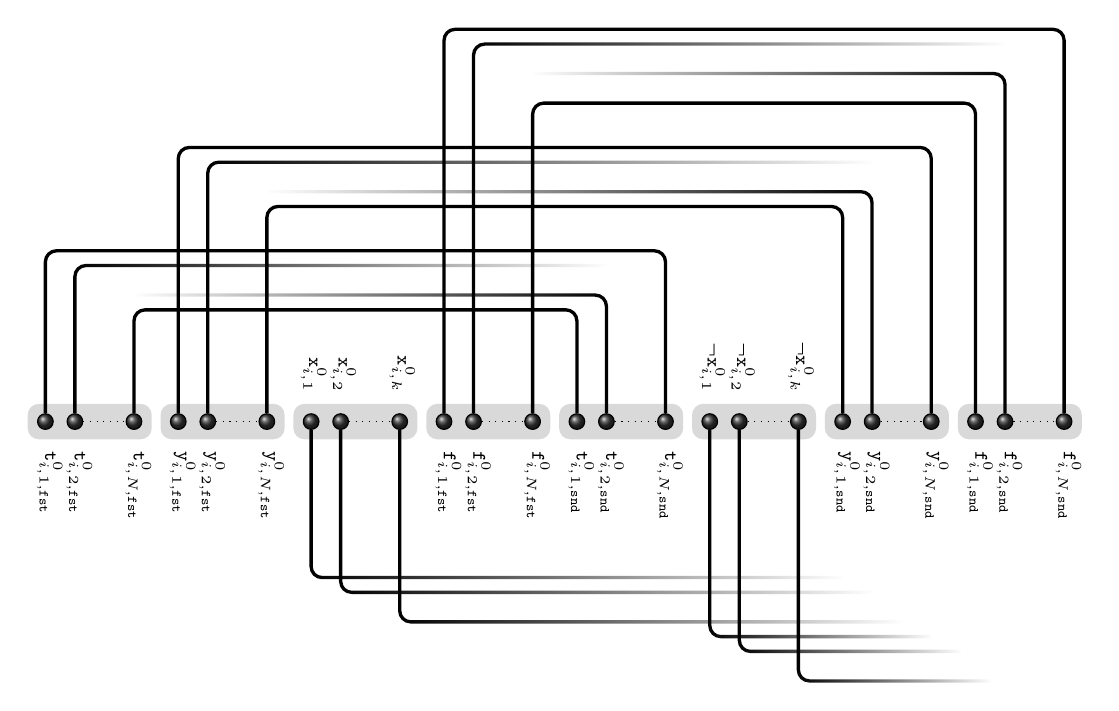
\begin{tikzpicture}
    [
    scale=.375,
    my vertex/.style={basic vertex,
    minimum size=1pt,
    inner sep=2pt,
    ball color=black!80},
    ]
    % vertices

    % p left
    \begin{scope}[]
      \fill [rounded corners, black!15] (-0.6,-0.6) -- (-0.6,0.6) --
      (3.6,0.6)   -- (3.6,-0.6) --
      cycle;
      \node [
      my vertex,
      label={[text depth=0ex,label distance=0.25cm,rotate=-90]right:{\scriptsize $\texttt{t}^{0}_{i,1,\LEFT}$}}
      ] (P1l) at (0,0) {};
      \node [
      my vertex,
      label={[text depth=0ex,label distance=0.25cm,rotate=-90]right:{\scriptsize $\texttt{t}^{0}_{i,2,\LEFT}$}}
      ] (P2l) at (1,0) {};
      \node [
      my vertex,
      label={[text depth=0ex,label distance=0.25cm,rotate=-90]right:{\scriptsize $\texttt{t}^{0}_{i,N,\LEFT}$}}
      ] (PNl) at (3,0) {};
      \path [draw,dotted] (P2l) -- (PNl);
    \end{scope}

    % r left
    \begin{scope}[xshift=4.5cm]
      \fill [rounded corners, black!15] (-0.6,-0.6) -- (-0.6,0.6) --
      (3.6,0.6)   -- (3.6,-0.6) --
      cycle;
      \node [
      my vertex,
      label={[text depth=0ex,label distance=0.25cm,rotate=-90]right:{\scriptsize $\texttt{y}^{0}_{i,1,\LEFT}$}}
      ] (R1l) at (0,0) {};
      \node [
      my vertex,
      label={[text depth=0ex,label distance=0.25cm,rotate=-90]right:{\scriptsize $\texttt{y}^{0}_{i,2,\LEFT}$}}
      ] (R2l) at (1,0) {};
      \node [
      my vertex,
      label={[text depth=0ex,label distance=0.25cm,rotate=-90]right:{\scriptsize $\texttt{y}^{0}_{i,N,\LEFT}$}}
      ] (RNl) at (3,0) {};
      \path [draw,dotted] (R2l) -- (RNl);
    \end{scope}

    % x
    \begin{scope}[xshift=9cm]
      \fill [rounded corners, black!15] (-0.6,-0.6) -- (-0.6,0.6) --
      (3.6,0.6)   -- (3.6,-0.6) --
      cycle;
      \node [
      my vertex,
      label={[text depth=2.5ex,label distance=0.25cm,rotate=-90]left:{\scriptsize $\texttt{x}^{0}_{i,1}$}}
      ] (X1) at (0,0) {};
      \node [
      my vertex,
      label={[text depth=2.5ex,label distance=0.25cm,rotate=-90]left:{\scriptsize $\texttt{x}^{0}_{i,2}$}}
      ] (X2) at (1,0) {};
      \node [
      my vertex,
      label={[text depth=2.5ex,label distance=0.25cm,rotate=-90]left:{\scriptsize $\texttt{x}^{0}_{i,k}$}}
      ] (Xk) at (3,0) {};
      \path [draw,dotted] (X2) -- (Xk);
    \end{scope}

    % q left
    \begin{scope}[xshift=13.5cm]
      \fill [rounded corners, black!15] (-0.6,-0.6) -- (-0.6,0.6) --
      (3.6,0.6)   -- (3.6,-0.6) --
      cycle;
      \node [
      my vertex,
      label={[text depth=0ex,label distance=0.25cm,rotate=-90]right:{\scriptsize $\texttt{f}^{0}_{i,1,\LEFT}$}}
      ] (Q1l) at (0,0) {};
      \node [
      my vertex,
      label={[text depth=0ex,label distance=0.25cm,rotate=-90]right:{\scriptsize $\texttt{f}^{0}_{i,2,\LEFT}$}}
      ] (Q2l) at (1,0) {};
      \node [
      my vertex,
      label={[text depth=0ex,label distance=0.25cm,rotate=-90]right:{\scriptsize $\texttt{f}^{0}_{i,N,\LEFT}$}}
      ] (QNl) at (3,0) {};
      \path [draw,dotted] (Q2l) -- (QNl);
    \end{scope}

    % p right
    \begin{scope}[xshift=18cm]
      \fill [rounded corners, black!15] (-0.6,-0.6) -- (-0.6,0.6) --
      (3.6,0.6)   -- (3.6,-0.6) --
      cycle;
      \node [
      my vertex,
      label={[text depth=0ex,label distance=0.25cm,rotate=-90]right:{\scriptsize $\texttt{t}^{0}_{i,1,\RIGHT}$}}
      ] (P1r) at (0,0) {};
      \node [
      my vertex,
      label={[text depth=0ex,label distance=0.25cm,rotate=-90]right:{\scriptsize $\texttt{t}^{0}_{i,2,\RIGHT}$}}
      ] (P2r) at (1,0) {};
      \node [
      my vertex,
      label={[text depth=0ex,label distance=0.25cm,rotate=-90]right:{\scriptsize $\texttt{t}^{0}_{i,N,\RIGHT}$}}
      ] (PNr) at (3,0) {};
      \path [draw,dotted] (P2r) -- (PNr);
    \end{scope}

    % neg x
    \begin{scope}[xshift=22.5cm]
      \fill [rounded corners, black!15] (-0.6,-0.6) -- (-0.6,0.6) --
      (3.6,0.6)   -- (3.6,-0.6) --
      cycle;
      \node [
      my vertex,
      label={[text depth=2.5ex,label distance=0.25cm,rotate=-90]left:{\scriptsize $\neg\texttt{x}^{0}_{i,1}$}}
      ] (nX1) at (0,0) {};
      \node [
      my vertex,
      label={[text depth=2.5ex,label distance=0.25cm,rotate=-90]left:{\scriptsize $\neg\texttt{x}^{0}_{i,2}$}}
      ] (nX2) at (1,0) {};
      \node [
      my vertex,
      label={[text depth=2.5ex,label distance=0.25cm,rotate=-90]left:{\scriptsize $\neg\texttt{x}^{0}_{i,k}$}}
      ] (nXk) at (3,0) {};
      \path [draw,dotted] (nX2) -- (nXk);
    \end{scope}

    % r right
    \begin{scope}[xshift=27cm]
      \fill [rounded corners, black!15] (-0.6,-0.6) -- (-0.6,0.6) --
      (3.6,0.6)   -- (3.6,-0.6) --
      cycle;
      \node [
      my vertex,
      label={[text depth=0ex,label distance=0.25cm,rotate=-90]right:{\scriptsize $\texttt{y}^{0}_{i,1,\RIGHT}$}}
      ] (R1r) at (0,0) {};
      \node [
      my vertex,
      label={[text depth=0ex,label distance=0.25cm,rotate=-90]right:{\scriptsize $\texttt{y}^{0}_{i,2,\RIGHT}$}}
      ] (R2r) at (1,0) {};
      \node [
      my vertex,
      label={[text depth=0ex,label distance=0.25cm,rotate=-90]right:{\scriptsize $\texttt{y}^{0}_{i,N,\RIGHT}$}}
      ] (RNr) at (3,0) {};
      \path [draw,dotted] (R2r) -- (RNr);
    \end{scope}

    % q right
    \begin{scope}[xshift=31.5cm]
      \fill [rounded corners, black!15] (-0.6,-0.6) -- (-0.6,0.6) --
      (3.6,0.6)   -- (3.6,-0.6) --
      cycle;
      \node [
      my vertex,
      label={[text depth=0ex,label distance=0.25cm,rotate=-90]right:{\scriptsize $\texttt{f}^{0}_{i,1,\RIGHT}$}}
      ] (Q1r) at (0,0) {};
      \node [
      my vertex,
      label={[text depth=0ex,label distance=0.25cm,rotate=-90]right:{\scriptsize $\texttt{f}^{0}_{i,2,\RIGHT}$}}
      ] (Q2r) at (1,0) {};
      \node [
      my vertex,
      label={[text depth=0ex,label distance=0.25cm,rotate=-90]right:{\scriptsize $\texttt{f}^{0}_{i,N,\RIGHT}$}}
      ] (QNr) at (3,0) {};
      \path [draw,dotted] (Q2r) -- (QNr);
    \end{scope}

    % edges
    \path [edge]
    (P1l.north) -- ++(0,5.5) -- ($(PNr.north)+(0,5.5)$) -- (PNr.north);
    \path [edge,path fading=east]
    (P2l.north) -- ++(0,5) --  ($(P2r.north)+(0,5)$);
    \path [edge,path fading=west]
    (P2r.north) -- ++(0,4) -- ($(PNl.north)+(0,4)$);
    \path [edge]
    (PNl.north) -- ($(PNl.north)+(0,3.5)$) -- ($(P1r.north)+(0,3.5)$) -- (P1r.north);

    \path [edge]
    (Q1l.north) -- ++(0,13) -- ($(QNr.north)+(0,13)$) -- (QNr.north);
    \path [edge,path fading=east]
    (Q2l.north) -- ++(0,12.5) --  ($(Q2r.north)+(0,12.5)$);
    \path [edge,path fading=west]
    (Q2r.north) -- ++(0,11.5) -- ($(QNl.north)+(0,11.5)$);
    \path [edge]
    (QNl.north) -- ($(QNl.north)+(0,10.5)$) -- ($(Q1r.north)+(0,10.5)$) -- (Q1r.north);

    \path [edge]
    (R1l.north) -- ++(0,9) -- ($(RNr.north)+(0,9)$) -- (RNr.north);
    \path [edge,path fading=east]
    (R2l.north) -- ++(0,8.5) --  ($(R2r.north)+(0,8.5)$);
    \path [edge,path fading=west]
    (R2r.north) -- ++(0,7.5) -- ($(RNl.north)+(0,7.5)$);
    \path [edge]
    (RNl.north) -- ($(RNl.north)+(0,7)$) -- ($(R1r.north)+(0,7)$) -- (R1r.north);

    \path [edge,path fading=east] (X1.south) -- ++(0,-5) -- ++(18,0);
    \path [edge,path fading=east] (X2.south) -- ++(0,-5.5) -- ++(18,0);
    \path [edge,path fading=east] (Xk.south) -- ++(0,-6.5) -- ++(17,0);

    \path [edge,path fading=east] (nX1.south) -- ++(0,-7) -- ++(7.5,0);
    \path [edge,path fading=east] (nX2.south) -- ++(0,-7.5) -- ++(7.5,0);
    \path [edge,path fading=east] (nXk.south) -- ++(0,-8.5) -- ++(6.5,0);

    %\node [text width=2cm,anchor=west] at (31,-7) {\scriptsize Towards the clause gadgets};
  \end{tikzpicture}

  \caption{\label{fig-3-linear-graph-splitting-variable-gadget-0}%
  A variable gadget $\texttt{Var}^{0}_{i}$ where
  $\texttt{x}^{0}_{i,1}, \texttt{x}^{0}_{i,2}, \dots, \texttt{x}^{0}_{i,k}$
  (resp.
  $\neg\texttt{x}^{0}_{i,1}, \neg\texttt{x}^{0}_{i,2}, \dots, \neg\texttt{x}^{0}_{i,k}$
  )
  represent the vertices of $\texttt{X}^{0}_{i}$ (resp. $\neg\texttt{X}^{0}_{i}$) with
  $k = \OCCURRENCE(x_i) = \OCCURRENCE_1(x_i) + 2\,\OCCURRENCE_2(x_i) + \OCCURRENCE_3(x_i)$.
  The intra-gadget edges of $E^{0}_{\texttt{Var}, i} =
  E^{0}_{\texttt{Var}, i, \texttt{t}} \cup
  E^{0}_{\texttt{Var}, i, \texttt{f}} \cup
  E^{0}_{\texttt{Var}, i, \texttt{y}}$ are shown together
  with the left endpoint parts of the associated inter-gadget edges of
  $E^{0}_{\texttt{Var},\texttt{Cls}}$.
  }% end caption
\end{figure}


  \begin{figure}
  \centering

  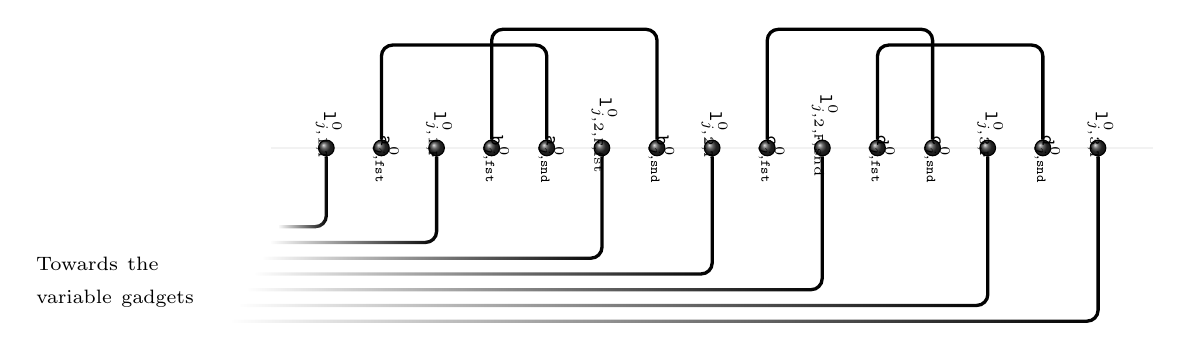
\begin{tikzpicture}
    [
      scale=.2,
      my vertex/.style={basic vertex,
      minimum size=1pt,
      inner sep=2pt,
      ball color=black!80},
    ]
    \path [draw,color=black!5] (0,0) -- (56,0);

    % vertices
    \foreach \i/\l [evaluate=\i as \x using \i*3.5] in
    {
      2/\texttt{a}^{0}_{j,\LEFT},
      4/\texttt{b}^{0}_{j,\LEFT},
      5/\texttt{a}^{0}_{j,\RIGHT},
      7/\texttt{b}^{0}_{j,\RIGHT},
      9/\texttt{c}^{0}_{j,\LEFT},
      11/\texttt{d}^{0}_{j,\LEFT},
      12/\texttt{c}^{0}_{j,\RIGHT},
      14/\texttt{d}^{0}_{j,\RIGHT}
    }
    {
    \node [
    my vertex,
    label={[text depth=0ex,anchor=center,label distance=0.15cm,rotate=-90]right:{\scriptsize $\l$}}
    ] (V\i) at (\x,0) {};
    }
    \foreach \i/\l [evaluate=\i as \x using \i*3.5] in
    {
      1/\texttt{l}^{0}_{j,1,\TRUE},
      3/\texttt{l}^{0}_{j,1,\FALSE},
      6/\texttt{l}^{0}_{j,2,\FALSE,\FST},
      8/\texttt{l}^{0}_{j,2,\TRUE},
      10/\texttt{l}^{0}_{j,2,\FALSE,\SND},
      13/\texttt{l}^{0}_{j,3,\FALSE},
      15/\texttt{l}^{0}_{j,3,\TRUE}
    }
    {

    \node [
      my vertex,
      label={[text depth=2.5ex,anchor=center,label distance=0.15cm,rotate=-90]left:{\scriptsize $\l$}}
    ] (V\i) at (\x,0) {};
    }

    % edges
    \path [edge] (V2.north) -- ++ (0,6) -- ($(V5.north)+(0,6)$) -- (V5.north);
    \path [edge] (V4.north) -- ++ (0,7) -- ($(V7.north)+(0,7)$) -- (V7.north);
    \path [edge] (V9.north) -- ++ (0,7) -- ($(V12.north)+(0,7)$) -- (V12.north);
    \path [edge] (V11.north) -- ++ (0,6) -- ($(V14.north)+(0,6)$) -- (V14.north);

    % incoming edges
    \draw [edge,path fading=west] (V1) -- ++(0,-5) -- +(-3,0) node {};
    \draw [edge,path fading=west] (V3) -- ++(0,-6) -- +(-10.5,0) node {};
    \draw [edge,path fading=west] (V6)  -- ++(0,-7)  -- +(-21.5,0) node {};
    \draw [edge,path fading=west] (V8)  -- ++(0,-8)  -- +(-29,0) node {};
    \draw [edge,path fading=west] (V10) -- ++(0,-9) -- +(-36.5,0) node {};
    \draw [edge,path fading=west] (V13) -- ++(0,-10) -- +(-47.5,0) node {};
    \draw [edge,path fading=west] (V15) -- ++(0,-11) -- +(-55,0) node {};

    \node [text width=2.5cm,anchor=west] at (-15.5,-8.5) {\scriptsize Towards the variable gadgets};

  \end{tikzpicture}

  \caption{\label{fig-3-linear-graph-splitting-clause-gadget-0}%
  A clause gadget $\texttt{Cls}^{0}_{j}$.
  The intra-gadget edges of
  $E^{0}_{\texttt{Cls}, j} =
  E^{0}_{\texttt{Cls}, j, \texttt{a}} \cup
  E^{0}_{\texttt{Cls}, j, \texttt{b}} \cup
  E^{0}_{\texttt{Cls}, j, \texttt{c}} \cup
  E^{0}_{\texttt{Cls}, j, \texttt{d}}$ are shown together
  with the right endpoint parts of the associated inter-gadget edges of
  $E^{0}_{\texttt{Var},\texttt{Cls}}$.
  }% end caption
\end{figure}


  % matching \mathcal{M}1
  \medskip
  \textbf{Defining the target matching $\mathcal{M}{1} = (V^{1}, E^{1})$}
  \medskip
  % \begin{mdframed}
    Define
    \begin{alignat*} {2}
      V^{1} &= \texttt{Var}^{1} \cup \texttt{Cls}^{1}
      &\quad&\text{with $\texttt{Var}^{1} < \texttt{C}^{1}$}
      \\
      \texttt{Var}^{1} &= \bigcup_{i=1}^{n} \texttt{Var}^{1}_{i}
      &&\text{with $\texttt{Var}^{1}_1 < \texttt{Var}^{1}_2 < \cdots < \texttt{Var}^{1}_n$}
      \\
      \texttt{Cls}^{1} &= \bigcup_{j=1}^{m} \texttt{Cls}^{1}_{j}
      &&\text{with $\texttt{Cls}^{1}_1 < \texttt{Cls}^{1}_2 < \cdots < \texttt{Cls}^{1}_m$.}
    \end{alignat*}
    For $1 \leq i \leq n$, define
    \begin{alignat*}{2}
      \texttt{Var}^{1}_{i} &=
      \texttt{TF}^{1}_{i,\LEFT} \cup \texttt{X}^{1}_{i} \cup \texttt{TF}^{1}_{i,\RIGHT}
      &&\text{with $\texttt{TF}^{1}_{i,\LEFT} < \texttt{X}^{1}_{i} < \texttt{TF}^{1}_{i,\RIGHT}$},
      \\
      \texttt{TF}^{1}_{i,\LEFT}
      &=
      \{\texttt{tf}^{1}_{i,j,\LEFT} : 1 \leq j \leq N\},
      &&
      \\
      \texttt{X}^{1}_{i}
      &=
      \{\texttt{x}^{1}_{i,j} : \text{$x_{i}$ or $\overline{x_{i}}$ occurs in clause $c_{j}$}\},
      &&
      \\
      \texttt{TF}^{1}_{i,\RIGHT}
      &=
      \{\texttt{tf}^{1}_{i,j,\RIGHT} : 1 \leq j \leq N\},
      &&
      \\
      \texttt{Cls}^{0}_{j}
      &=
      \{
      \texttt{l}^{1}_{j,1},
      \texttt{l}^{1}_{j,2},
      \texttt{l}^{1}_{j,3},
      \texttt{ab}^{1}_{j,\LEFT},
      \texttt{cd}^{1}_{j,\LEFT},
      \texttt{ab}^{1}_{j,\RIGHT},
      \texttt{cd}^{1}_{j,\RIGHT}
      \}
      &&
    \end{alignat*}
    with
    $
    \texttt{l}^{1}_{j,1} <
    \texttt{ab}^{1}_{j,\LEFT} <
    \texttt{ab}^{1}_{j,\RIGHT} <
    \texttt{l}^{1}_{j,2} <
    \texttt{cd}^{1}_{j,\LEFT} <
    \texttt{cd}^{1}_{j,\RIGHT} <
    \texttt{l}^{1}_{j,3}
    $.
    The vertices in $\texttt{Var}^{1}_{i}$ are ordered according to their second coordinate
    (always written $j$ in the above definitions).

    We now turn to defining the edges $E^{1}$ of the matching $\mathcal{M}{1}$.
    Define
    \begin{align*}
      E^{1} &= E^{1}_{\texttt{Var}} \cup E^{1}_{\texttt{Var},\texttt{Cls}} \cup E^{1}_{\texttt{Cls}},
      \\
      E^{1}_{\texttt{Var}} &= \bigcup_{i=1}^{n} E^{1}_{\texttt{Var}, i},
      \\
      \forall 1\leq i \leq n,\quad
      E^{1}_{\texttt{Var}, i} &= \bigcup_{k=1}^{N} (\texttt{TF}^{1}_{i,k}, \texttt{TF}^{1}_{i,N-k+1}),
      \\
      E^{1}_{\texttt{Cls}} &= \bigcup_{j=1}^{m} E^{1}_{\texttt{Cls}, j},
      \\
      \forall 1\leq j \leq m,\quad
      E^{1}_{\texttt{Cls}, j} &=
      \{
      (\texttt{ab}^{1}_{j,\LEFT}, \texttt{ab}^{1}_{j,\RIGHT}),
      (\texttt{cd}^{1}_{j,\LEFT}, \texttt{cd}^{1}_{j,\RIGHT})
      \}\text{.}
    \end{align*}
    What is left is to define $E^{1}_{\texttt{Var},\texttt{Cls}}$.
    For every $\texttt{l}^{1}_{j, 1} \in V^{1}_{\texttt{Cls}}$
    (resp. $\texttt{l}^{1}_{j, 2} \in V^{1}_{\texttt{Cls}}$ and
    $\texttt{l}^{1}_{j, 3} \in V^{1}_{\texttt{Cls}}$)
    we add
    the edge $(\texttt{x}^{1}_{i,j}, \texttt{l}^{1}_{j, 1})$
    (resp. $(\texttt{x}^{2}_{i,j}, \texttt{l}^{1}_{j, 1})$ and
    $(\texttt{x}^{3}_{i,j}, \texttt{l}^{1}_{j, 1})$)
    to $E^{1}_{\texttt{Var},\texttt{Cls}}$
    if the first (resp. second and third) literal of the clause $c_{j}$
    is the positive or the negative literal $x_{i}$.
  % \end{mdframed}

  The construction of the matching $\mathcal{M}{0}$ is illustrated
  in Figure~\ref{fig-3-linear-graph-splitting-variable-gadget-1} and
  Figure~\ref{fig-3-linear-graph-splitting-clause-gadget-1}.

  \begin{figure}
  \centering

  \begin{tikzpicture}
    [
    scale=.375,
    my vertex/.style={basic vertex,
    minimum size=1pt,
    inner sep=2pt,
    ball color=black!80},
    ]
    % vertices

    % TF left
    \begin{scope}[]
      \fill [rounded corners, black!15] (-0.6,-0.6) -- (-0.6,0.6) --
      (3.6,0.6)   -- (3.6,-0.6) --
      cycle;
      \node [
      my vertex,
      label={[text depth=0ex,label distance=0.25cm,rotate=-90]right:{\scriptsize $\texttt{tf}^{1}_{i,1,\LEFT}$}}
      ] (TF1l) at (0,0) {};
      \node [
      my vertex,
      label={[text depth=0ex,label distance=0.25cm,rotate=-90]right:{\scriptsize $\texttt{tf}^{1}_{i,2,\LEFT}$}}
      ] (TF2l) at (1,0) {};
      \node [
      my vertex,
      label={[text depth=0ex,label distance=0.25cm,rotate=-90]right:{\scriptsize $\texttt{tf}^{1}_{i,N,\LEFT}$}}
      ] (TFNl) at (3,0) {};
      \path [draw,dotted] (TF2l) -- (TFNl);
    \end{scope}

    % x
    \begin{scope}[xshift=4.5cm]
      \fill [rounded corners, black!15] (-0.6,-0.6) -- (-0.6,0.6) --
      (3.6,0.6)   -- (3.6,-0.6) --
      cycle;
      \node [
      my vertex,
      label={[text depth=2.5ex,label distance=0.25cm,rotate=-90]left:{\scriptsize $\texttt{x}^{1}_{i,1}$}}
      ] (X1) at (0,0) {};
      \node [
      my vertex,
      label={[text depth=2.5ex,label distance=0.25cm,rotate=-90]left:{\scriptsize $\texttt{x}^{1}_{i,2}$}}
      ] (X2) at (1,0) {};
      \node [
      my vertex,
      label={[text depth=2.5ex,label distance=0.25cm,rotate=-90]left:{\scriptsize $\texttt{x}^{1}_{i,k}$}}
      ] (Xk) at (3,0) {};
      \path [draw,dotted] (X2) -- (Xk);
    \end{scope}

    % p right
    \begin{scope}[xshift=9cm]
      \fill [rounded corners, black!15] (-0.6,-0.6) -- (-0.6,0.6) --
      (3.6,0.6)   -- (3.6,-0.6) --
      cycle;
      \node [
      my vertex,
      label={[text depth=0ex,label distance=0.25cm,rotate=-90]right:{\scriptsize $\texttt{tf}^{1}_{i,1,\RIGHT}$}}
      ] (TF1r) at (0,0) {};
      \node [
      my vertex,
      label={[text depth=0ex,label distance=0.25cm,rotate=-90]right:{\scriptsize $\texttt{tf}^{1}_{i,2,\RIGHT}$}}
      ] (TF2r) at (1,0) {};
      \node [
      my vertex,
      label={[text depth=0ex,label distance=0.25cm,rotate=-90]right:{\scriptsize $\texttt{tf}^{1}_{i,N,\RIGHT}$}}
      ] (TFNr) at (3,0) {};
      \path [draw,dotted] (TF2r) -- (TFNr);
    \end{scope}

    % edges
    \path [edge]
    (TF1l.north) -- ++(0,5.5) -- ($(TFNr.north)+(0,5.5)$) -- (TFNr.north);
    \path [edge,path fading=east]
    (TF2l.north) -- ++(0,5) --  ($(TF2r.north)+(0,5)$);
    \path [edge,path fading=west]
    (TF2r.north) -- ++(0,4) -- ($(TFNl.north)+(0,4)$);
    \path [edge]
    (TFNl.north) -- ($(PNl.north)+(0,3.5)$) -- ($(TF1r.north)+(0,3.5)$) -- (TF1r.north);

    \path [edge,path fading=east] (X1.south) -- ++(0,-5) -- ++(13,0);
    \path [edge,path fading=east] (X2.south) -- ++(0,-5.5) -- ++(13,0);
    \path [edge,path fading=east] (Xk.south) -- ++(0,-6.5) -- ++(12,0);

    %\node [text width=2cm,anchor=west] at (19,-6) {\scriptsize Towards the clause gadgets};
  \end{tikzpicture}

  \caption{\label{fig-3-linear-graph-splitting-variable-gadget-1}%
  A variable gadget $\texttt{Var}^{1}_{i}$ where
  $\texttt{x}^{1}_{i,1}, \texttt{x}^{1}_{i,2}, \dots, \texttt{x}^{1}_{i,k}$
  represent the vertices of $\texttt{X}^{1}_{i}$ with
  $k = \OCCURRENCE(x_i) = \OCCURRENCE_1(x_i) + 2\,\OCCURRENCE_2(x_i) + \OCCURRENCE_3(x_i)$.
  The intra-gadget edges of $E^{1}_{\texttt{Var}, i} =
  E^{1}_{\texttt{Var}, i, \texttt{tf}} $ are shown together
  with the left endpoint parts of the associated inter-gadget edges of
  $E^{1}_{\texttt{Var},\texttt{Cls}}$.
  }% end caption
\end{figure}


  \begin{figure}
  \centering

  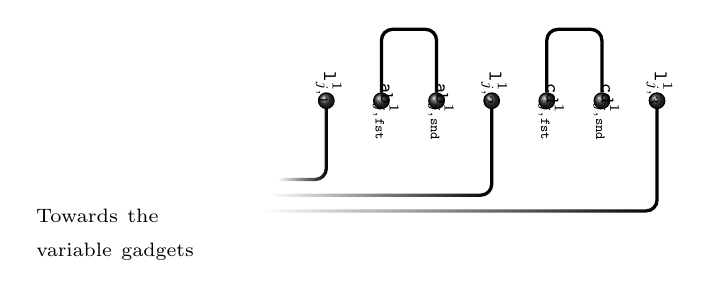
\begin{tikzpicture}
  [
    scale=.2,
    my vertex/.style={basic vertex,
                      minimum size=1pt,
                      inner sep=2pt,
                      ball color=black!80},
  ]
    % vertices
    \foreach \i/\l [evaluate=\i as \x using \i*3.5] in
      {
        2/\texttt{ab}^{1}_{j,\LEFT},
        3/\texttt{ab}^{1}_{j,\RIGHT},
        5/\texttt{cd}^{1}_{j,\LEFT},
        6/\texttt{cd}^{1}_{j,\RIGHT}
      }
    {
    \node [
      my vertex,
      label={[text depth=0ex,anchor=center,label distance=0.15cm,rotate=-90]right:{\scriptsize $\l$}}
    ] (V\i) at (\x,0) {};
    }

    % vertices
    \foreach \i/\l [evaluate=\i as \x using \i*3.5] in
      {
        1/\texttt{l}^{1}_{j,1},
        4/\texttt{l}^{1}_{j,2},
        7/\texttt{l}^{1}_{j,3}
      }
    {
    \node [
      my vertex,
      label={[text depth=2.5ex,anchor=center,label distance=0.15cm,rotate=-90]left:{\scriptsize $\l$}}
    ] (V\i) at (\x,0) {};    }

    % edges
    \path [edge] (V2.north) -- ++ (0,4) -- ($(V3.north)+(0,4)$) -- (V3.north);
    \path [edge] (V5.north) -- ++ (0,4) -- ($(V6.north)+(0,4)$) -- (V6.north);

    % incoming edges
    \draw [edge,path fading=west] (V1) -- ++(0,-5) -- +(-3,0) node {};
    \draw [edge,path fading=west] (V4) -- ++(0,-6) -- +(-14,0) node {};
    \draw [edge,path fading=west] (V7)  -- ++(0,-7)  -- +(-25,0) node {};

    \node [text width=2.5cm,anchor=west] at (-15.5,-8.5) {\scriptsize Towards the variable gadgets};

  \end{tikzpicture}

  \caption{\label{fig-3-linear-graph-splitting-clause-gadget-1}%
    A clause gadget $\texttt{Cls}^{1}_{j}$.
    The two intra-gadget edges of
    $E^{1}_{\texttt{Cls}, j} =
    \{(\texttt{ab}^{1}_{j, \LEFT}, \texttt{ab}^{1}_{j, \RIGHT}),
    (\texttt{cd}^{1}_{j, \LEFT}, \texttt{cd}^{1}_{j, \RIGHT})\}$
    are shown together
    with the right endpoint parts of the associated inter-gadget edges of
    $E^{1}_{\texttt{Var},\texttt{Cls}}$.
  }% end caption
\end{figure}


  % matching \mathcal{M}2
  \medskip
  \textbf{Defining the target matching $\mathcal{M}{2} = (V^{2}, E^{2})$}
  \medskip

  % \begin{mdframed}
    The matching $\mathcal{M}{2}$ is identical to $\mathcal{M}{1}$ except that it does not
    contain any edge in $E^{2}_{\texttt{Cls}}$.
    More formally,
    define
    \begin{alignat*} {2}
      V^{2} &= \texttt{Var}^{2} \cup \texttt{Cls}^{2}
      &\quad&\text{with $\texttt{Var}^{2} < \texttt{Cls}^{2}$}
      \\
      \texttt{Var}^{2} &= \bigcup_{i=1}^{n} \texttt{Var}^{2}_{i}
      &&\text{with $\texttt{Var}^{2}_1 < \texttt{Var}^{2}_2 < \dots < \texttt{Var}^{2}_n$}
      \\
      \texttt{Cls}^{2} &= \bigcup_{j=1}^{m} \texttt{Cls}^{2}_{j}
      &&\text{with $\texttt{Cls}^{2}_1 < \texttt{Cls}^{2}_2 < \dots < \texttt{Cls}^{2}_m$.}
      \\
      \forall, 1 \leq i \leq n,\;
      \texttt{Var}^{2}_{i} &= \texttt{TF}^{2}_{i,\LEFT} \cup \texttt{X}^{2}_{i} \cup \texttt{TF}^{2}_{i,\RIGHT}
      &&\text{with $\texttt{TF}^{2}_{i,\LEFT} < \texttt{X}^{2}_{i} < \texttt{TF}^{2}_{i,\RIGHT}$}
      \\
      \texttt{TF}^{2}_{i,\LEFT}
      &=
      \{\texttt{TF}^{2}_{i,j,\LEFT} : 1 \leq j \leq N\}
      &&\\
      \texttt{X}^{2}_{i}
      &=
      \{\texttt{x}^{2}_{i,j} : \text{$x_{i}$ or $\overline{x_{i}}$ occurs in $c_{j}$}\}
      &&\\
      \texttt{TF}^{2}_{i,\RIGHT}
      &=
      \{\texttt{TF}^{2}_{i,j,\RIGHT} : 1 \leq j \leq N\}
      &&
      \\
      \texttt{Cls}^{2}_{j}
      &=
      \{
      \texttt{l}^{2}_{j,1},
      \texttt{l}^{2}_{j,2},
      \texttt{l}^{2}_{j,3}
      \}
      &&\text{with $\texttt{l}^{2}_{j,1} < \texttt{l}^{2}_{j,2} < \texttt{l}^{2}_{j,3}$}
      \\
    \end{alignat*}
    The vertices in $\texttt{Var}^{2}_{i}$ are ordered according to their second coordinate
    (always written $j$ in the above definitions).

    We now turn to defining the edges $E^{2}$ of the matching $\mathcal{M}{2}$.
    Define
    \begin{align*}
      E^{2} &= E^{2}_{\texttt{Var}} \cup E^{2}_{\texttt{Var},\texttt{Cls}},
      \\
      E^{2}_{\texttt{Var}} &= \bigcup_{i=1}^{n} E^{2}_{\texttt{Var}, i},
      \\
      \forall 1\leq i \leq n,\quad
      E^{2}_{\texttt{Var}, i} &= \bigcup_{k=1}^{N} (\texttt{TF}^{2}_{i,k}, \texttt{TF}^{2}_{i,N-k+1})\text{.}
    \end{align*}
    As for $E^{2}_{\texttt{Var},\texttt{Cls}}$,
    \begin{itemize}
      \item
      for every $\texttt{l}^{2}_{j, 1} \in V^{2}_{\texttt{Cls}}$,
      we add
      the edge $(\texttt{x}^{2}_{i,j}, \texttt{l}^{2}_{j, 1})$
      to $E^{2}_{\texttt{Var},\texttt{Cls}}$
      if $c_{j}[1] = x_{i}$ or $c_{j}[1] = \overline{x_{i}}$.
      \item
      for every $\texttt{l}^{2}_{j, 2} \in V^{2}_{\texttt{Cls}}$,
      we add
      the edge $(\texttt{x}^{2}_{i,j}, \texttt{l}^{2}_{j, 1})$
      to $E^{2}_{\texttt{Var},\texttt{Cls}}$
      if $c_{j}[2] = x_{i}$ or $c_{j}[2] = \overline{x_{i}}$.
      \item
      for every $\texttt{l}^{2}_{j, 3} \in V^{2}_{\texttt{Cls}}$,
      we add
      the edge $(\texttt{x}^{3}_{i,j}, \texttt{l}^{2}_{j, 1})$
      to $E^{2}_{\texttt{Var},\texttt{Cls}}$
      if $c_{j}[3] = x_{i}$ or $c_{j}[3] = \overline{x_{i}}$.
    \end{itemize}
  % \end{mdframed}

  The construction of the matching $\mathcal{M}{2}$ is illustrated
  in Figure~\ref{fig-3-linear-graph-splitting-variable-gadget-2}.

  \begin{figure}
  \centering

  \begin{tikzpicture}
    [
    scale=.375,
    my vertex/.style={basic vertex,
    minimum size=1pt,
    inner sep=2pt,
    ball color=black!80},
    ]
    % vertices

    % TF left
    \begin{scope}[]
      \fill [rounded corners, black!15] (-0.6,-0.6) -- (-0.6,0.6) --
      (3.6,0.6)   -- (3.6,-0.6) --
      cycle;
      \node [
      my vertex,
      label={[text depth=0ex,label distance=0.25cm,rotate=-90]right:{\scriptsize $\texttt{tf}^{2}_{i,1,\LEFT}$}}
      ] (TF1l) at (0,0) {};
      \node [
      my vertex,
      label={[text depth=0ex,label distance=0.25cm,rotate=-90]right:{\scriptsize $\texttt{tf}^{2}_{i,2,\LEFT}$}}
      ] (TF2l) at (1,0) {};
      \node [
      my vertex,
      label={[text depth=0ex,label distance=0.25cm,rotate=-90]right:{\scriptsize $\texttt{tf}^{2}_{i,N,\LEFT}$}}
      ] (TFNl) at (3,0) {};
      \path [draw,dotted] (TF2l) -- (TFNl);
    \end{scope}

    % x
    \begin{scope}[xshift=4.5cm]
      \fill [rounded corners, black!15] (-0.6,-0.6) -- (-0.6,0.6) --
      (3.6,0.6)   -- (3.6,-0.6) --
      cycle;
      \node [
      my vertex,
      label={[text depth=2.5ex,label distance=0.25cm,rotate=-90]left:{\scriptsize $\texttt{x}^{2}_{i,1}$}}
      ] (X1) at (0,0) {};
      \node [
      my vertex,
      label={[text depth=2.5ex,label distance=0.25cm,rotate=-90]left:{\scriptsize $\texttt{x}^{2}_{i,2}$}}
      ] (X2) at (1,0) {};
      \node [
      my vertex,
      label={[text depth=2.5ex,label distance=0.25cm,rotate=-90]left:{\scriptsize $\texttt{x}^{2}_{i,k}$}}
      ] (Xk) at (3,0) {};
      \path [draw,dotted] (X2) -- (Xk);
    \end{scope}

    % p right
    \begin{scope}[xshift=9cm]
      \fill [rounded corners, black!15] (-0.6,-0.6) -- (-0.6,0.6) --
      (3.6,0.6)   -- (3.6,-0.6) --
      cycle;
      \node [
      my vertex,
      label={[text depth=0ex,label distance=0.25cm,rotate=-90]right:{\scriptsize $\texttt{tf}^{2}_{i,1,\RIGHT}$}}
      ] (TF1r) at (0,0) {};
      \node [
      my vertex,
      label={[text depth=0ex,label distance=0.25cm,rotate=-90]right:{\scriptsize $\texttt{tf}^{2}_{i,2,\RIGHT}$}}
      ] (TF2r) at (1,0) {};
      \node [
      my vertex,
      label={[text depth=0ex,label distance=0.25cm,rotate=-90]right:{\scriptsize $\texttt{tf}^{2}_{i,N,\RIGHT}$}}
      ] (TFNr) at (3,0) {};
      \path [draw,dotted] (TF2r) -- (TFNr);
    \end{scope}

    % edges
    \path [edge]
    (TF1l.north) -- ++(0,5.5) -- ($(TFNr.north)+(0,5.5)$) -- (TFNr.north);
    \path [edge,path fading=east]
    (TF2l.north) -- ++(0,5) --  ($(TF2r.north)+(0,5)$);
    \path [edge,path fading=west]
    (TF2r.north) -- ++(0,4) -- ($(TFNl.north)+(0,4)$);
    \path [edge]
    (TFNl.north) -- ($(PNl.north)+(0,3.5)$) -- ($(TF1r.north)+(0,3.5)$) -- (TF1r.north);

    \path [edge,path fading=east] (X1.south) -- ++(0,-5) -- ++(13,0);
    \path [edge,path fading=east] (X2.south) -- ++(0,-5.5) -- ++(13,0);
    \path [edge,path fading=east] (Xk.south) -- ++(0,-6.5) -- ++(12,0);

    %\node [text width=2cm,anchor=west] at (19,-6) {\scriptsize Towards the clause gadgets};
  \end{tikzpicture}

  \caption{\label{fig-3-linear-graph-splitting-variable-gadget-2}%
  A variable gadget $\texttt{Var}^{2}_{i}$ where
  $\texttt{x}^{2}_{i,1}, \texttt{x}^{2}_{i,2}, \dots, \texttt{x}^{2}_{i,k}$
  represent the vertices of $\texttt{X}^{2}_{i}$ with
  $k = \OCCURRENCE(x_i) = \OCCURRENCE_1(x_i) + 2\,\OCCURRENCE_2(x_i) + \OCCURRENCE_3(x_i)$.
  The intra-gadget edges of $E^{2}_{\texttt{Var}, i} =
  E^{2}_{\texttt{Var}, i, \texttt{tf}} $ are shown together
  with the left endpoint parts of the associated inter-gadget edges of
  $E^{2}_{\texttt{Var},\texttt{Cls}}$.
  }% end caption
\end{figure}


  % matching \mathcal{M}3
  \medskip
  \textbf{Defining the target matching $\mathcal{M}{3} = (V^{3}, E^{3})$}
  \medskip

  % \begin{mdframed}
    Define
    \begin{alignat*}{2}
      V^{3} &= \texttt{Var}^{3} \cup \texttt{C}^{3},
      &\quad&\text{$\texttt{Var}^{3} < \texttt{Cls}^{3}$,}
      \\
      \texttt{Var}^{3} &= \bigcup_{i=1}^{n} \texttt{Var}^{3}_{i},
      &&\text{$\texttt{Var}^{3}_1 < \texttt{Var}^{3}_2 < \cdots < \texttt{Var}^{3}_n$,}
      \\
      \texttt{Cls}^{3} &= \bigcup_{j=1}^{m} \texttt{Cls}^{3}_{j},
      &&\text{$\texttt{Cls}^{3}_1 < \texttt{Cls}^{3}_2 < \cdots < \texttt{Cls}^{3}_m$.}
    \end{alignat*}
    where
    \begin{alignat*}{3}
      &\forall \leq i \leq n,\;&
      \texttt{Var}^{3}_{i} &= \texttt{Y}^{3}_{i,\LEFT} \cup \texttt{X}^{3}_{i} \cup \texttt{Y}^{3}_{i,\RIGHT},
      &\quad&\text{$\texttt{Y}^{3}_{i,\LEFT} < \texttt{X}^{3}_{i} < \texttt{Y}^{3}_{i,\RIGHT}$},
      \\
      &\forall \leq i \leq n,\;&
      \texttt{Y}^{3}_{i,\LEFT}
      &=
      \{\texttt{y}^{3}_{i,j,\LEFT} : 1 \leq j \leq N\},
      &&
      \\
      &\forall \leq i \leq n,\;&
      \texttt{X}^{3}_{i}
      &=
      \{\texttt{x}^{3}_{i,j,\FST}, \texttt{x}^{3}_{i,j,\SND} :
      \text{$x_{i} = c_{j}[2]$ or $\overline{x_{i}} = c_{j}[2]$}\},
      &&
      \\
      &\forall \leq i \leq n,\;&
      \texttt{Y}^{3}_{i,\RIGHT}
      &=
      \{\texttt{y}^{3}_{i,j,\RIGHT} : 1 \leq j \leq N\},
      &&
      \\
      &&\texttt{Cls}^{3}_{j}
      &=
      \{
      \texttt{l}^{3}_{j},
      \}
      \cup
      \{
      \texttt{ab}^{3}_{j,\LEFT},
      \texttt{cd}^{3}_{j,\LEFT},
      \texttt{ab}^{3}_{j,\RIGHT},
      \texttt{cd}^{3}_{j,\RIGHT}
      \}
      &&
    \end{alignat*}
    with
    $
    \texttt{ab}^{3}_{j,\LEFT} <
    \texttt{ab}^{3}_{j,\RIGHT} <
    \texttt{l}^{3}_{j} <
    \texttt{cd}^{3}_{j,\LEFT} <
    \texttt{cd}^{3}_{j,1,\RIGHT}
    $.
    All subsets
    $\texttt{Y}^{3}_{i,\LEFT}$, $\texttt{X}^{3}_{i}$ and $\texttt{Y}^{3}_{i,\RIGHT}$,
    are ordered according to the second coordinate index of the vertices
    (always written $j$ in the above definitions).

    For the edges $E^{3}$ of the matching $\mathcal{M}{3}$,
    define
    \begin{alignat*}{2}
      &&
      E^{3} &= E^{3}_{\texttt{Var}} \cup E^{3}_{\texttt{Var},\texttt{Cls}} \cup E^{3}_{\texttt{Cls}}
      \\
      &&
      E^{3}_{\texttt{Var}} &= \bigcup_{i=1}^{n} E^{3}_{\texttt{Var}, i}
      \\
      &\forall 1\leq i \leq n,\quad&
      E^{3}_{\texttt{Var}, 3} &= \bigcup_{k=1}^{N} (\texttt{y}^{3}_{i,k}, \texttt{y}^{3}_{i,N-k+1})
      \\
      &&
      E^{3}_{\texttt{Cls}} &= \bigcup_{j=1}^{m} E^{3}_{\texttt{Cls}, j}
      \\
      &\forall 1\leq j \leq m,\quad&
      E^{3}_{\texttt{Cls}, j} &=
      \{
      (\texttt{ab}^{3}_{j,\LEFT}, \texttt{ab}^{3}_{j,\RIGHT})
      \}\text{.}
    \end{alignat*}
    As for $E^{3}_{\texttt{Var},\texttt{Cls}}$,
    for every $\texttt{l}^{3}_{j} \in \texttt{Cls}^{3}_{j}$,
    we add the edge
    $(\texttt{x}^{3}_{i,j}, \texttt{l}^{3}_{j}) \in E^{3}_{\texttt{Var},\texttt{Cls}}$
    if $x_{i} = c_{j}[2]$ or $\overline{x_{i}} = c_{j}[2]$.
  % \end{mdframed}

  \bigskip

  We now claim that the $3$-CNF formula $\phi$ is satisfiable
  if and only if
  $\mathcal{M}{0}$ is $(\mathcal{M}{1}, \mathcal{M}{2}, \mathcal{M}{3})$-colorable.

  $(\Rightarrow)$
  Suppose that the $3$-CNF formula $\phi$ is satisfiable, and
  let $\gamma : X \to \{\FALSE, \TRUE\}$ be a satisfying assignment
  for $\phi$.
  Let $\COLOR_1$, $\COLOR_2$ and $\COLOR_3$ be three distinct colors.
  We define a mapping
  $\rho : V^{0} \to \{\COLOR_1, \COLOR_2, \COLOR_3\}$ as follows.

  \paragraph*{Gadgets $\texttt{Var}^{0}_{i}$}

  \begin{alignat*}{4}
    &\forall 1 \leq i \leq n, \forall 1 \leq j \leq N\;,
    &\quad
    \rho(\texttt{t}^{0}_{i, j, \LEFT}) &= \rho(\texttt{t}^{0}_{i, j, \RIGHT}) &=&
    \begin{cases}
      \COLOR_1 & \text{if $\gamma(x_i) = \TRUE$}\\
      \COLOR_2 & \text{if $\gamma(x_i) = \FALSE$}
    \end{cases}
    \\
    &\forall 1 \leq i \leq n, \forall 1 \leq j \leq N\;,
    &\quad
    \rho(\texttt{f}^{0}_{i, j, \LEFT}) &= \rho(\texttt{f}^{0}_{i, j, \RIGHT}) &=&
    \begin{cases}
      \COLOR_1 & \text{if $\gamma(x_i) = \FALSE$}\\
      \COLOR_2 & \text{if $\gamma(x_i) = \TRUE$}
    \end{cases}
    \\
    &\forall 1 \leq i \leq n, \forall 1 \leq j \leq N\;,
    &\quad
    \rho(\texttt{y}^{0}_{i, j, \LEFT}) &= \rho(\texttt{y}^{0}_{i, j, \RIGHT}) &=&
    \COLOR_3
    \\
    &\forall 1 \leq i \leq n, \forall 1 \leq j \leq \OCCURRENCE(x_i)\;,
    &\quad
    \rho(\texttt{x}^{0}_{i, 1, j}) &= \rho(\texttt{x}^{0}_{i, 3, j}) &=&
    \begin{cases}
      \COLOR_1 & \text{if $\gamma(x_i) = \TRUE$}\\
      \COLOR_2 & \text{if $\gamma(x_i) = \FALSE$}
    \end{cases}
    \\
    &\forall 1 \leq i \leq n, \forall 1 \leq j \leq \OCCURRENCE(x_i)\;,
    &\quad
    \rho(\neg\texttt{x}^{0}_{i, 1, j}) &= \rho(\neg\texttt{x}^{0}_{i, 3, j}) &=&
    \begin{cases}
      \COLOR_1 & \text{if $\gamma(x_i) = \FALSE$}\\
      \COLOR_2 & \text{if $\gamma(x_i) = \TRUE$}
    \end{cases}
    \\
  \end{alignat*}

  \paragraph*{Gadgets $\texttt{Cls}^{0}_{j}$}

  It can be checked that
  \begin{itemize}
    \item
    every vertex of $\mathcal{M}{0}$ is assigned exactly one color,
    \item
    every edge of $\mathcal{M}{0}$ connect two vertices with the same color,
    \item
    the subgraph of $\mathcal{M}{0}$ induced by color $\COLOR_1$
    (resp. $\COLOR_2$ and $\COLOR_3$) is isomorphic to $\mathcal{M}{1}$
    (resp. $\mathcal{M}{2}$ and $\mathcal{M}{3}$).
  \end{itemize}

  $(\Leftarrow)$
  Suppose now that $\mathcal{M}{0}$ is $(\mathcal{M}{1}, \mathcal{M}{2}, \mathcal{M}{3})$-colorable.
  We show how to construct a satifsying assignment
  $\gamma : X \to \{\FALSE, \TRUE\}$ for $\phi$.


  \begin{figure}
  \centering

  \begin{subfigure}[b]{\textwidth}
    \centering
    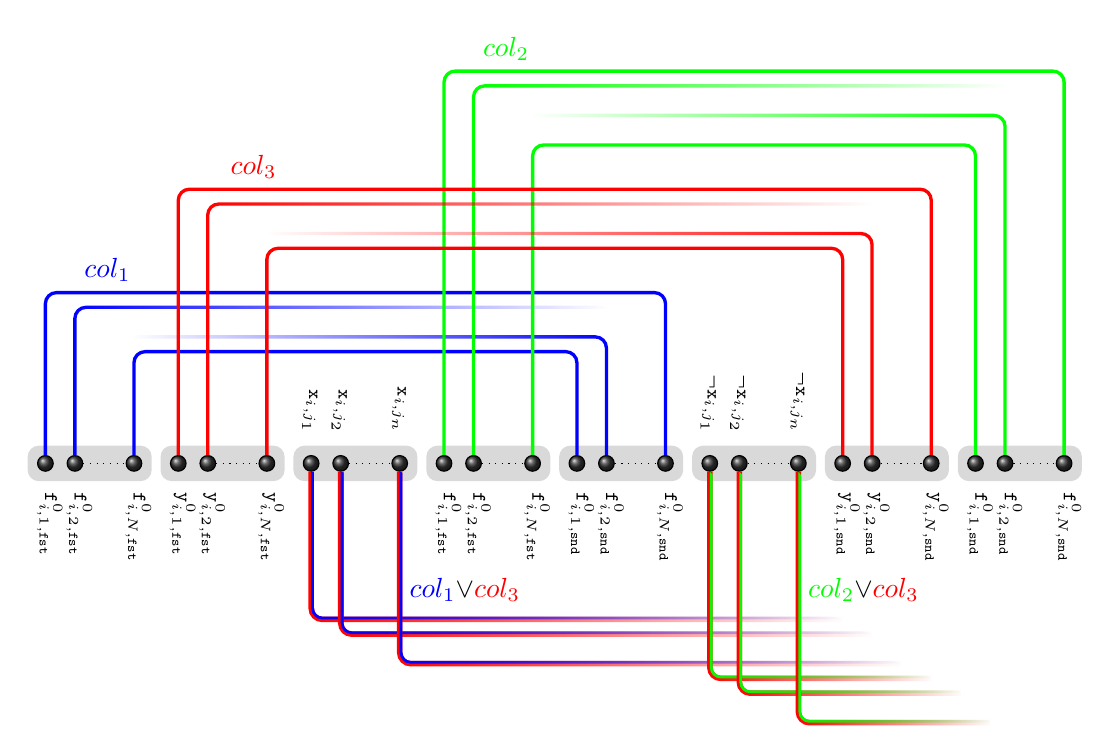
\begin{tikzpicture}
      [
      scale=.375,
      my vertex/.style={basic vertex,
      minimum size=1pt,
      inner sep=2pt,
      ball color=black!80},
      ]
      % vertices

      % p left
      \begin{scope}[]
        \fill [rounded corners, black!15] (-0.6,-0.6) -- (-0.6,0.6) --
        (3.6,0.6)   -- (3.6,-0.6) --
        cycle;
        \node [
        my vertex,
        label={[text depth=-1.75ex,label distance=0.25cm,rotate=-90]right:{\scriptsize $\texttt{f}^0_{i,1,\LEFT}$}}
        ] (T1l) at (0,0) {};
        \node [
        my vertex,
        label={[text depth=-1.75ex,label distance=0.25cm,rotate=-90]right:{\scriptsize $\texttt{f}^0_{i,2,\LEFT}$}}
        ] (T2l) at (1,0) {};
        \node [
        my vertex,
        label={[text depth=-1.75ex,label distance=0.25cm,rotate=-90]right:{\scriptsize $\texttt{f}^0_{i,N,\LEFT}$}}
        ] (TNl) at (3,0) {};
        \path [draw,dotted] (T2l) -- (TNl);
      \end{scope}

      % r left
      \begin{scope}[xshift=4.5cm]
        \fill [rounded corners, black!15] (-0.6,-0.6) -- (-0.6,0.6) --
        (3.6,0.6)   -- (3.6,-0.6) --
        cycle;
        \node [
        my vertex,
        label={[text depth=-1.75ex,label distance=0.25cm,rotate=-90]right:{\scriptsize $\texttt{y}^0_{i,1,\LEFT}$}}
        ] (Y1l) at (0,0) {};
        \node [
        my vertex,
        label={[text depth=-1.75ex,label distance=0.25cm,rotate=-90]right:{\scriptsize $\texttt{y}^0_{i,2,\LEFT}$}}
        ] (Y2l) at (1,0) {};
        \node [
        my vertex,
        label={[text depth=-1.75ex,label distance=0.25cm,rotate=-90]right:{\scriptsize $\texttt{y}^0_{i,N,\LEFT}$}}
        ] (YNl) at (3,0) {};
        \path [draw,dotted] (Y2l) -- (YNl);
      \end{scope}

      % x
      \begin{scope}[xshift=9cm]
        \fill [rounded corners, black!15] (-0.6,-0.6) -- (-0.6,0.6) --
        (3.6,0.6)   -- (3.6,-0.6) --
        cycle;
        \node [
        my vertex,
        label={[text depth=1.75ex,label distance=0.25cm,rotate=-90]left:{\scriptsize $\texttt{x}_{i,j_1}$}}
        ] (X1) at (0,0) {};
        \node [
        my vertex,
        label={[text depth=1.75ex,label distance=0.25cm,rotate=-90]left:{\scriptsize $\texttt{x}_{i,j_2}$}}
        ] (X2) at (1,0) {};
        \node [
        my vertex,
        label={[text depth=1.75ex,label distance=0.25cm,rotate=-90]left:{\scriptsize $\texttt{x}_{i,j_n}$}}
        ] (Xk) at (3,0) {};
        \path [draw,dotted] (X2) -- (Xk);
      \end{scope}

      % q left
      \begin{scope}[xshift=13.5cm]
        \fill [rounded corners, black!15] (-0.6,-0.6) -- (-0.6,0.6) --
        (3.6,0.6)   -- (3.6,-0.6) --
        cycle;
        \node [
        my vertex,
        label={[text depth=-1.75ex,label distance=0.25cm,rotate=-90]right:{\scriptsize $\texttt{f}^0_{i,1,\LEFT}$}}
        ] (F1l) at (0,0) {};
        \node [
        my vertex,
        label={[text depth=-1.75ex,label distance=0.25cm,rotate=-90]right:{\scriptsize $\texttt{f}^0_{i,2,\LEFT}$}}
        ] (F2l) at (1,0) {};
        \node [
        my vertex,
        label={[text depth=-1.75ex,label distance=0.25cm,rotate=-90]right:{\scriptsize $\texttt{f}^0_{i,N,\LEFT}$}}
        ] (FNl) at (3,0) {};
        \path [draw,dotted] (F2l) -- (FNl);
      \end{scope}

      % p right
      \begin{scope}[xshift=18cm]
        \fill [rounded corners, black!15] (-0.6,-0.6) -- (-0.6,0.6) --
        (3.6,0.6)   -- (3.6,-0.6) --
        cycle;
        \node [
        my vertex,
        label={[text depth=-1.75ex,label distance=0.25cm,rotate=-90]right:{\scriptsize $\texttt{f}^0_{i,1,\RIGHT}$}}
        ] (T1r) at (0,0) {};
        \node [
        my vertex,
        label={[text depth=-1.75ex,label distance=0.25cm,rotate=-90]right:{\scriptsize $\texttt{f}^0_{i,2,\RIGHT}$}}
        ] (T2r) at (1,0) {};
        \node [
        my vertex,
        label={[text depth=-1.75ex,label distance=0.25cm,rotate=-90]right:{\scriptsize $\texttt{f}^0_{i,N,\RIGHT}$}}
        ] (TNr) at (3,0) {};
        \path [draw,dotted] (T2r) -- (TNr);
      \end{scope}

      % neg x
      \begin{scope}[xshift=22.5cm]
        \fill [rounded corners, black!15] (-0.6,-0.6) -- (-0.6,0.6) --
        (3.6,0.6)   -- (3.6,-0.6) --
        cycle;
        \node [
        my vertex,
        label={[text depth=1.75ex,label distance=0.25cm,rotate=-90]left:{\scriptsize $\neg\texttt{x}_{i,j_1}$}}
        ] (nX1) at (0,0) {};
        \node [
        my vertex,
        label={[text depth=1.75ex,label distance=0.25cm,rotate=-90]left:{\scriptsize $\neg\texttt{x}_{i,j_2}$}}
        ] (nX2) at (1,0) {};
        \node [
        my vertex,
        label={[text depth=1.75ex,label distance=0.25cm,rotate=-90]left:{\scriptsize $\neg\texttt{x}_{i,j_n}$}}
        ] (nXk) at (3,0) {};
        \path [draw,dotted] (nX2) -- (nXk);
      \end{scope}

      % r right
      \begin{scope}[xshift=27cm]
        \fill [rounded corners, black!15] (-0.6,-0.6) -- (-0.6,0.6) --
        (3.6,0.6)   -- (3.6,-0.6) --
        cycle;
        \node [
        my vertex,
        label={[text depth=-1.75ex,label distance=0.25cm,rotate=-90]right:{\scriptsize $\texttt{y}^0_{i,1,\RIGHT}$}}
        ] (Y1r) at (0,0) {};
        \node [
        my vertex,
        label={[text depth=-1.75ex,label distance=0.25cm,rotate=-90]right:{\scriptsize $\texttt{y}^0_{i,2,\RIGHT}$}}
        ] (Y2r) at (1,0) {};
        \node [
        my vertex,
        label={[text depth=-1.75ex,label distance=0.25cm,rotate=-90]right:{\scriptsize $\texttt{y}^0_{i,N,\RIGHT}$}}
        ] (YNr) at (3,0) {};
        \path [draw,dotted] (Y2r) -- (YNr);
      \end{scope}

      % q right
      \begin{scope}[xshift=31.5cm]
        \fill [rounded corners, black!15] (-0.6,-0.6) -- (-0.6,0.6) --
        (3.6,0.6)   -- (3.6,-0.6) --
        cycle;
        \node [
        my vertex,
        label={[text depth=-1.75ex,label distance=0.25cm,rotate=-90]right:{\scriptsize $\texttt{f}^0_{i,1,\RIGHT}$}}
        ] (F1r) at (0,0) {};
        \node [
        my vertex,
        label={[text depth=-1.75ex,label distance=0.25cm,rotate=-90]right:{\scriptsize $\texttt{f}^0_{i,2,\RIGHT}$}}
        ] (F2r) at (1,0) {};
        \node [
        my vertex,
        label={[text depth=-1.75ex,label distance=0.25cm,rotate=-90]right:{\scriptsize $\texttt{f}^0_{i,N,\RIGHT}$}}
        ] (FNr) at (3,0) {};
        \path [draw,dotted] (F2r) -- (FNr);
      \end{scope}

      % edges
      \path [edge,color=blue]
      (T1l.north) -- ++(0,5.5) -- ($(TNr.north)+(0,5.5)$) node [pos=0.1,above] {$\COLOR_1$} -- (TNr.north);
      \path [edge,color=blue,path fading=east]
      (T2l.north) -- ++(0,5) --  ($(T2r.north)+(0,5)$);
      \path [edge,color=blue,path fading=west]
      (T2r.north) -- ++(0,4) -- ($(TNl.north)+(0,4)$);
      \path [edge,color=blue]
      (TNl.north) -- ($(TNl.north)+(0,3.5)$) -- ($(T1r.north)+(0,3.5)$) -- (T1r.north);

      \path [edge,color=green]
      (F1l.north) -- ++(0,13) -- ($(FNr.north)+(0,13)$) node [pos=0.1,above] {$\COLOR_2$} -- (FNr.north);
      \path [edge,color=green,path fading=east]
      (F2l.north) -- ++(0,12.5) --  ($(F2r.north)+(0,12.5)$);
      \path [edge,color=green,path fading=west]
      (F2r.north) -- ++(0,11.5) -- ($(FNl.north)+(0,11.5)$);
      \path [edge,color=green]
      (FNl.north) -- ($(FNl.north)+(0,10.5)$) -- ($(F1r.north)+(0,10.5)$) -- (F1r.north);

      \path [edge,color=red]
      (Y1l.north) -- ++(0,9) -- ($(YNr.north)+(0,9)$) node [pos=0.1,above] {$\COLOR_3$} -- (YNr.north);
      \path [edge,color=red,path fading=east]
      (Y2l.north) -- ++(0,8.5) --  ($(Y2r.north)+(0,8.5)$);
      \path [edge,color=red,path fading=west]
      (Y2r.north) -- ++(0,7.5) -- ($(YNl.north)+(0,7.5)$);
      \path [edge,color=red]
      (YNl.north) -- ($(YNl.north)+(0,7)$) -- ($(Y1r.north)+(0,7)$) -- (Y1r.north);

      \path [edge,side by side={red}{blue},path fading=east] (X1.south) -- ++(0,-5) -- ++(18,0);
      \path [edge,side by side={red}{blue},path fading=east] (X2.south) -- ++(0,-5.5) -- ++(18,0);
      \path [edge,side by side={red}{blue},path fading=east] (Xk.south) -- ++(0,-6.5) -- ++(17,0);
      \node [text width=2cm] at ($(Xk.south)+(3,-4)$) {$\color{blue}{\COLOR_1} \color{black}{\vee} \color{red}{\COLOR_3}$};

      \path [edge,side by side={red}{green},path fading=east] (nX1.south) -- ++(0,-7) -- ++(7.5,0);
      \path [edge,side by side={red}{green},path fading=east] (nX2.south) -- ++(0,-7.5) -- ++(7.5,0);
      \path [edge,side by side={red}{green},path fading=east] (nXk.south)  -- ++(0,-8.5) -- ++(6.5,0);
      \node [text width=2cm] at ($(nXk.south)+(3,-4)$) {$\color{green}{\COLOR_2} \color{black}{\vee} \color{red}{\COLOR_3}$};

      %\node [text width=2cm,anchor=west] at (31,-7) {\scriptsize Towards the clause gadgets};
    \end{tikzpicture}
    \caption{Setting $\rho(x_i) = \text{true}$ in variable gadget $\texttt{Var}^{0}_{i}$.}
  \end{subfigure}

  \vspace{.5cm}

  \begin{subfigure}[b]{\textwidth}
    \centering
    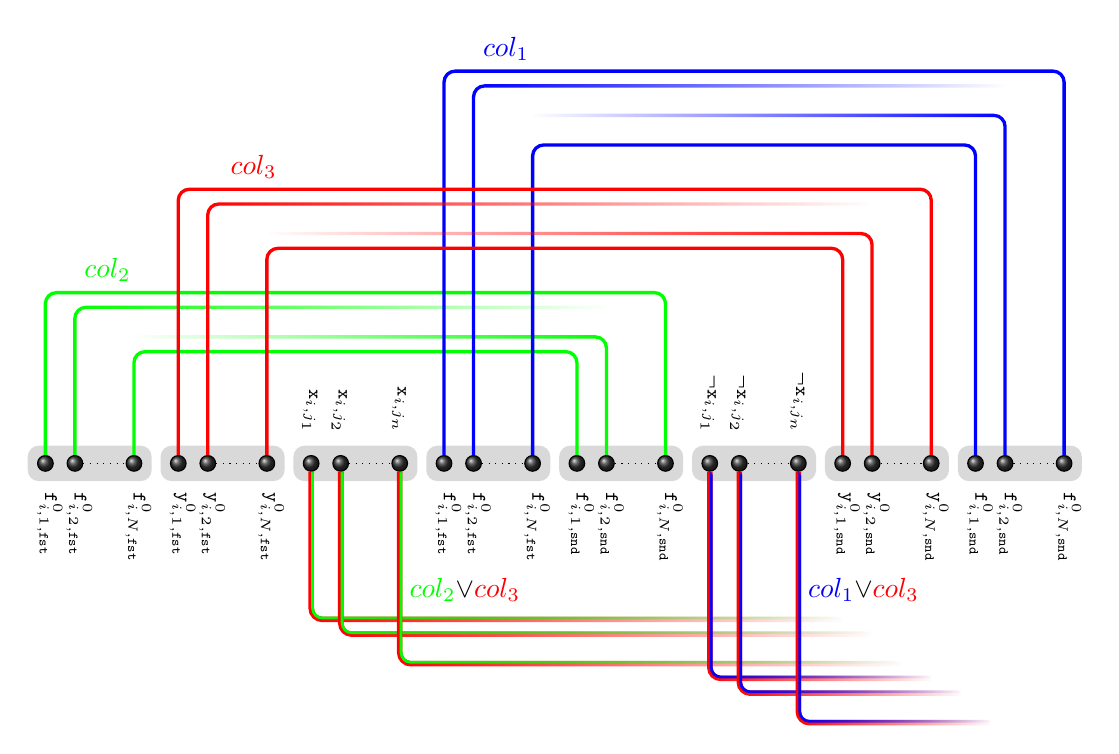
\begin{tikzpicture}
      [
      scale=.375,
      my vertex/.style={basic vertex,
      minimum size=1pt,
      inner sep=2pt,
      ball color=black!80},
      ]
      % vertices

      % p left
      \begin{scope}[]
        \fill [rounded corners, black!15] (-0.6,-0.6) -- (-0.6,0.6) --
        (3.6,0.6)   -- (3.6,-0.6) --
        cycle;
        \node [
        my vertex,
        label={[text depth=-1.75ex,label distance=0.25cm,rotate=-90]right:{\scriptsize $\texttt{f}^0_{i,1,\LEFT}$}}
        ] (T1l) at (0,0) {};
        \node [
        my vertex,
        label={[text depth=-1.75ex,label distance=0.25cm,rotate=-90]right:{\scriptsize $\texttt{f}^0_{i,2,\LEFT}$}}
        ] (T2l) at (1,0) {};
        \node [
        my vertex,
        label={[text depth=-1.75ex,label distance=0.25cm,rotate=-90]right:{\scriptsize $\texttt{f}^0_{i,N,\LEFT}$}}
        ] (TNl) at (3,0) {};
        \path [draw,dotted] (T2l) -- (TNl);
      \end{scope}

      % r left
      \begin{scope}[xshift=4.5cm]
        \fill [rounded corners, black!15] (-0.6,-0.6) -- (-0.6,0.6) --
        (3.6,0.6)   -- (3.6,-0.6) --
        cycle;
        \node [
        my vertex,
        label={[text depth=-1.75ex,label distance=0.25cm,rotate=-90]right:{\scriptsize $\texttt{y}^0_{i,1,\LEFT}$}}
        ] (Y1l) at (0,0) {};
        \node [
        my vertex,
        label={[text depth=-1.75ex,label distance=0.25cm,rotate=-90]right:{\scriptsize $\texttt{y}^0_{i,2,\LEFT}$}}
        ] (Y2l) at (1,0) {};
        \node [
        my vertex,
        label={[text depth=-1.75ex,label distance=0.25cm,rotate=-90]right:{\scriptsize $\texttt{y}^0_{i,N,\LEFT}$}}
        ] (YNl) at (3,0) {};
        \path [draw,dotted] (Y2l) -- (YNl);
      \end{scope}

      % x
      \begin{scope}[xshift=9cm]
        \fill [rounded corners, black!15] (-0.6,-0.6) -- (-0.6,0.6) --
        (3.6,0.6)   -- (3.6,-0.6) --
        cycle;
        \node [
        my vertex,
        label={[text depth=1.75ex,label distance=0.25cm,rotate=-90]left:{\scriptsize $\texttt{x}_{i,j_1}$}}
        ] (X1) at (0,0) {};
        \node [
        my vertex,
        label={[text depth=1.75ex,label distance=0.25cm,rotate=-90]left:{\scriptsize $\texttt{x}_{i,j_2}$}}
        ] (X2) at (1,0) {};
        \node [
        my vertex,
        label={[text depth=1.75ex,label distance=0.25cm,rotate=-90]left:{\scriptsize $\texttt{x}_{i,j_n}$}}
        ] (Xk) at (3,0) {};
        \path [draw,dotted] (X2) -- (Xk);
      \end{scope}

      % q left
      \begin{scope}[xshift=13.5cm]
        \fill [rounded corners, black!15] (-0.6,-0.6) -- (-0.6,0.6) --
        (3.6,0.6)   -- (3.6,-0.6) --
        cycle;
        \node [
        my vertex,
        label={[text depth=-1.75ex,label distance=0.25cm,rotate=-90]right:{\scriptsize $\texttt{f}^0_{i,1,\LEFT}$}}
        ] (F1l) at (0,0) {};
        \node [
        my vertex,
        label={[text depth=-1.75ex,label distance=0.25cm,rotate=-90]right:{\scriptsize $\texttt{f}^0_{i,2,\LEFT}$}}
        ] (F2l) at (1,0) {};
        \node [
        my vertex,
        label={[text depth=-1.75ex,label distance=0.25cm,rotate=-90]right:{\scriptsize $\texttt{f}^0_{i,N,\LEFT}$}}
        ] (FNl) at (3,0) {};
        \path [draw,dotted] (F2l) -- (FNl);
      \end{scope}

      % p right
      \begin{scope}[xshift=18cm]
        \fill [rounded corners, black!15] (-0.6,-0.6) -- (-0.6,0.6) --
        (3.6,0.6)   -- (3.6,-0.6) --
        cycle;
        \node [
        my vertex,
        label={[text depth=-1.75ex,label distance=0.25cm,rotate=-90]right:{\scriptsize $\texttt{f}^0_{i,1,\RIGHT}$}}
        ] (T1r) at (0,0) {};
        \node [
        my vertex,
        label={[text depth=-1.75ex,label distance=0.25cm,rotate=-90]right:{\scriptsize $\texttt{f}^0_{i,2,\RIGHT}$}}
        ] (T2r) at (1,0) {};
        \node [
        my vertex,
        label={[text depth=-1.75ex,label distance=0.25cm,rotate=-90]right:{\scriptsize $\texttt{f}^0_{i,N,\RIGHT}$}}
        ] (TNr) at (3,0) {};
        \path [draw,dotted] (T2r) -- (TNr);
      \end{scope}


      % neg x
      \begin{scope}[xshift=22.5cm]
        \fill [rounded corners, black!15] (-0.6,-0.6) -- (-0.6,0.6) --
        (3.6,0.6)   -- (3.6,-0.6) --
        cycle;
        \node [
        my vertex,
        label={[text depth=1.75ex,label distance=0.25cm,rotate=-90]left:{\scriptsize $\neg\texttt{x}_{i,j_1}$}}
        ] (nX1) at (0,0) {};
        \node [
        my vertex,
        label={[text depth=1.75ex,label distance=0.25cm,rotate=-90]left:{\scriptsize $\neg\texttt{x}_{i,j_2}$}}
        ] (nX2) at (1,0) {};
        \node [
        my vertex,
        label={[text depth=1.75ex,label distance=0.25cm,rotate=-90]left:{\scriptsize $\neg\texttt{x}_{i,j_n}$}}
        ] (nXk) at (3,0) {};
        \path [draw,dotted] (nX2) -- (nXk);
      \end{scope}

      % r right
      \begin{scope}[xshift=27cm]
        \fill [rounded corners, black!15] (-0.6,-0.6) -- (-0.6,0.6) --
        (3.6,0.6)   -- (3.6,-0.6) --
        cycle;
        \node [
        my vertex,
        label={[text depth=-1.75ex,label distance=0.25cm,rotate=-90]right:{\scriptsize $\texttt{y}^0_{i,1,\RIGHT}$}}
        ] (Y1r) at (0,0) {};
        \node [
        my vertex,
        label={[text depth=-1.75ex,label distance=0.25cm,rotate=-90]right:{\scriptsize $\texttt{y}^0_{i,2,\RIGHT}$}}
        ] (Y2r) at (1,0) {};
        \node [
        my vertex,
        label={[text depth=-1.75ex,label distance=0.25cm,rotate=-90]right:{\scriptsize $\texttt{y}^0_{i,N,\RIGHT}$}}
        ] (YNr) at (3,0) {};
        \path [draw,dotted] (Y2r) -- (YNr);
      \end{scope}

      % q right
      \begin{scope}[xshift=31.5cm]
        \fill [rounded corners, black!15] (-0.6,-0.6) -- (-0.6,0.6) --
        (3.6,0.6)   -- (3.6,-0.6) --
        cycle;
        \node [
        my vertex,
        label={[text depth=-1.75ex,label distance=0.25cm,rotate=-90]right:{\scriptsize $\texttt{f}^0_{i,1,\RIGHT}$}}
        ] (F1r) at (0,0) {};
        \node [
        my vertex,
        label={[text depth=-1.75ex,label distance=0.25cm,rotate=-90]right:{\scriptsize $\texttt{f}^0_{i,2,\RIGHT}$}}
        ] (F2r) at (1,0) {};
        \node [
        my vertex,
        label={[text depth=-1.75ex,label distance=0.25cm,rotate=-90]right:{\scriptsize $\texttt{f}^0_{i,N,\RIGHT}$}}
        ] (FNr) at (3,0) {};
        \path [draw,dotted] (F2r) -- (FNr);
      \end{scope}

      % edges
      \path [edge,color=green]
      (T1l.north) -- ++(0,5.5) -- ($(TNr.north)+(0,5.5)$) node [pos=0.1,above] {$\COLOR_2$} -- (TNr.north);
      \path [edge,color=green,path fading=east]
      (T2l.north) -- ++(0,5) --  ($(T2r.north)+(0,5)$);
      \path [edge,color=green,path fading=west]
      (T2r.north) -- ++(0,4) -- ($(TNl.north)+(0,4)$);
      \path [edge,color=green]
      (TNl.north) -- ($(TNl.north)+(0,3.5)$) -- ($(T1r.north)+(0,3.5)$) -- (T1r.north);

      \path [edge,color=blue]
      (F1l.north) -- ++(0,13) -- ($(FNr.north)+(0,13)$) node [pos=0.1,above] {$\COLOR_1$} -- (FNr.north);
      \path [edge,color=blue,path fading=east]
      (F2l.north) -- ++(0,12.5) --  ($(F2r.north)+(0,12.5)$);
      \path [edge,color=blue,path fading=west]
      (F2r.north) -- ++(0,11.5) -- ($(FNl.north)+(0,11.5)$);
      \path [edge,color=blue]
      (FNl.north) -- ($(FNl.north)+(0,10.5)$) -- ($(F1r.north)+(0,10.5)$) -- (F1r.north);

      \path [edge,color=red]
      (Y1l.north) -- ++(0,9) -- ($(YNr.north)+(0,9)$) node [pos=0.1,above] {$\COLOR_3$} -- (YNr.north);
      \path [edge,color=red,path fading=east]
      (Y2l.north) -- ++(0,8.5) --  ($(Y2r.north)+(0,8.5)$);
      \path [edge,color=red,path fading=west]
      (Y2r.north) -- ++(0,7.5) -- ($(YNl.north)+(0,7.5)$);
      \path [edge,color=red]
      (YNl.north) -- ($(YNl.north)+(0,7)$) -- ($(Y1r.north)+(0,7)$) -- (Y1r.north);

      \path [edge,side by side={red}{green},path fading=east] (X1.south) -- ++(0,-5) -- ++(18,0);
      \path [edge,side by side={red}{green},path fading=east] (X2.south) -- ++(0,-5.5) -- ++(18,0);
      \path [edge,side by side={red}{green},path fading=east] (Xk.south) -- ++(0,-6.5) -- ++(17,0);
      \node [text width=2cm] at ($(Xk.south)+(3,-4)$) {$\color{green}{\COLOR_2} \color{black}{\vee} \color{red}{\COLOR_3}$};

      \path [edge,side by side={red}{blue},path fading=east] (nX1.south) -- ++(0,-7) -- ++(7.5,0);
      \path [edge,side by side={red}{blue},path fading=east] (nX2.south) -- ++(0,-7.5) -- ++(7.5,0);
      \path [edge,side by side={red}{blue},path fading=east] (nXk.south) -- ++(0,-8.5) -- ++(6.5,0);
      \node [text width=2cm] at ($(nXk.south)+(3,-4)$) {$\color{blue}{\COLOR_1} \color{black}{\vee} \color{red}{\COLOR_3}$};

      %\node [text width=2cm,anchor=west] at (31,-7) {\scriptsize Towards the clause gadgets};
    \end{tikzpicture}
    \caption{Setting $\rho(x_i) = \text{false}$ in variable gadget $\texttt{Var}^{0}_{i}$.}
  \end{subfigure}
\end{figure}


  
\begin{figure}
  \centering

  \begin{subfigure}[b]{\textwidth}
    \centering
    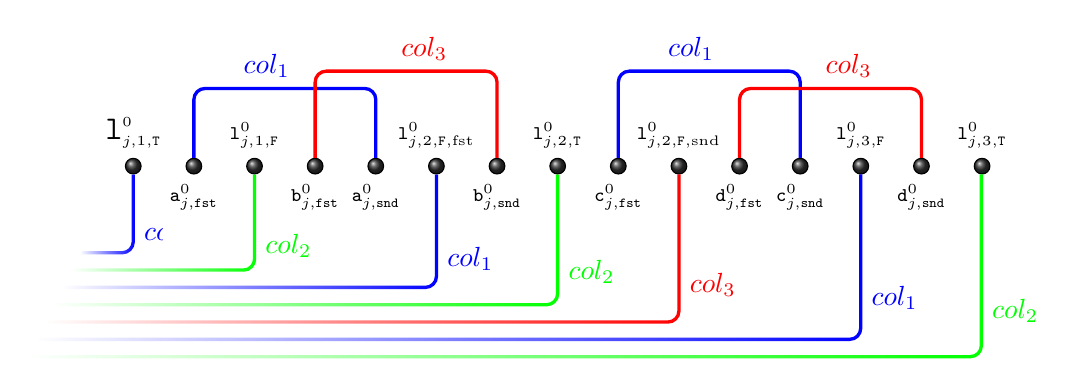
\begin{tikzpicture}
      [
      scale=.22,,,
      my vertex/.style={basic vertex,
      minimum size=1pt,
      inner sep=2pt,
      ball color=black!80},
      ]

      % vertices
      \foreach \i/\o/\l [evaluate=\i as \x using \i*3.5] in
      {
      1/above/\large\texttt{l}^0_{j,1,\TRUE},
      2/below/\texttt{a}^0_{j,\LEFT},
      3/above/\texttt{l}^0_{j,1,\FALSE},
      4/below/\texttt{b}^0_{j,\LEFT},
      5/below/\texttt{a}^0_{j,\RIGHT},
      6/above/\texttt{l}^0_{j,2,\FALSE,\FST},
      7/below/\texttt{b}^0_{j,\RIGHT},
      8/above/\texttt{l}^0_{j,2,\TRUE},
      9/below/\texttt{c}^0_{j,\LEFT},
      10/above/\texttt{l}^0_{j,2,\FALSE,\SND},
      11/below/\texttt{d}^0_{j,\LEFT},
      12/below/\texttt{c}^0_{j,\RIGHT},
      13/above/\texttt{l}^0_{j,3,\FALSE},
      14/below/\texttt{d}^0_{j,\RIGHT},
      15/above/\texttt{l}^0_{j,3,\TRUE}
      }
      {
      \node [my vertex,label=\o:{\scriptsize $\l$}] (V\i) at (\x,0) {};
      }

      % edges
      \path [edge,color=blue] (V2.north) -- ++ (0,4) --
      ($(V5.north)+(0,4)$) node [pos=0.4,above] {$\COLOR_1$} -- (V5.north);

      \path [edge,color=red] (V4.north) -- ++ (0,5) --
      ($(V7.north)+(0,5)$) node [pos=0.6,above] {$\COLOR_3$} -- (V7.north);

      \path [edge,color=blue] (V9.north) -- ++ (0,5) --
      ($(V12.north)+(0,5)$) node [pos=0.4,above] {$\COLOR_1$} -- (V12.north);

      \path [edge,color=red] (V11.north) -- ++ (0,4) --
      ($(V14.north)+(0,4)$) node [pos=0.6,above] {$\COLOR_3$} -- (V14.north);

      % incoming edges


      \draw [edge,color=green,path fading=west] (V3) -- node [pos=0.75,anchor=west] {$\COLOR_2$}
      ++(0,-6) -- +(-10.5,0);

      \draw [edge,color=blue,path fading=west] (V6) -- node [pos=0.75,anchor=west] {$\COLOR_1$}
      ++(0,-7) -- +(-21.5,0);

      \draw [edge,color=green,path fading=west] (V8) -- node [pos=0.75,anchor=west] {$\COLOR_2$}
      ++(0,-8)  -- +(-29,0);

      \draw [edge,color=red,path fading=west] (V10) -- node [pos=0.75,anchor=west] {$\COLOR_3$}
      ++(0,-9) -- +(-36.5,0);

      \draw [edge,color=blue,path fading=west] (V13) -- node [pos=0.75,anchor=west] {$\COLOR_1$}
      ++(0,-10) -- +(-47.5,0);

      \draw [edge,color=green,path fading=west] (V15) -- node [pos=0.75,anchor=west] {$\COLOR_2$}
      ++(0,-11) -- +(-55,0);

      \draw [edge,color=blue,path fading=west] (V1) -- node [pos=0.75,anchor=west] {$\COLOR_1$}
      ++(0,-5) -- +(-3,0);
      %\node [text width=2.5cm,anchor=west] at (-15.5,-8.5) {\scriptsize Towards the variable gadgets};

    \end{tikzpicture}
    \caption{%
    Clause gadget $\texttt{Cls}^{0}_{j}$ for clause $(\ell_{j,1} \vee \ell_{j,2} \vee \ell_{j,3})$
    in case the literals $\ell_{j,1}$, $\ell_{j,2}$ and $\ell_{j,3}$ evaluate to true, false and false,
    respectivelly, according to the satisfying assignment $f$.
    }% end caption  \end{subfigure}
  \end{subfigure}

  \vspace{.5cm}

  \begin{subfigure}[b]{\textwidth}
    \centering
    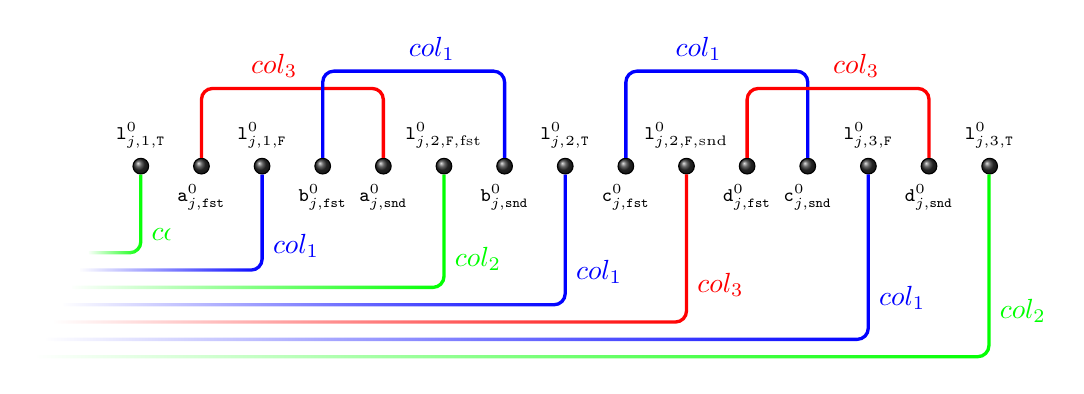
\begin{tikzpicture}
      [
      scale=.22,,,
      my vertex/.style={basic vertex,
      minimum size=1pt,
      inner sep=2pt,
      ball color=black!80},
      ]

      % vertices
      \foreach \i/\o/\l [evaluate=\i as \x using \i*3.5] in
      {
      1/above/\texttt{l}^0_{j,1,\TRUE},
      2/below/\texttt{a}^0_{j,\LEFT},
      3/above/\texttt{l}^0_{j,1,\FALSE},
      4/below/\texttt{b}^0_{j,\LEFT},
      5/below/\texttt{a}^0_{j,\RIGHT},
      6/above/\texttt{l}^0_{j,2,\FALSE,\FST},
      7/below/\texttt{b}^0_{j,\RIGHT},
      8/above/\texttt{l}^0_{j,2,\TRUE},
      9/below/\texttt{c}^0_{j,\LEFT},
      10/above/\texttt{l}^0_{j,2,\FALSE,\SND},
      11/below/\texttt{d}^0_{j,\LEFT},
      12/below/\texttt{c}^0_{j,\RIGHT},
      13/above/\texttt{l}^0_{j,3,\FALSE},
      14/below/\texttt{d}^0_{j,\RIGHT},
      15/above/\texttt{l}^0_{j,3,\TRUE}
      }
      {
      \node [my vertex,label=\o:{\scriptsize $\l$}] (V\i) at (\x,0) {};
      }

      % edges
      \path [edge,color=red] (V2.north) -- ++ (0,4) --
      ($(V5.north)+(0,4)$) node [pos=0.4,above] {$\COLOR_3$}  -- (V5.north);

      \path [edge,color=blue] (V4.north) -- ++ (0,5) --
      ($(V7.north)+(0,5)$) node [pos=0.6,above] {$\COLOR_1$} -- (V7.north);

      \path [edge,color=blue] (V9.north) -- ++ (0,5) --
      ($(V12.north)+(0,5)$) node [pos=0.4,above] {$\COLOR_1$} -- (V12.north);

      \path [edge,color=red] (V11.north) -- ++ (0,4) --
      ($(V14.north)+(0,4)$) node [pos=0.6,above] {$\COLOR_3$} -- (V14.north);

      % incoming edges
      \draw [edge,color=green,path fading=west] (V1) -- node [pos=0.75,anchor=west] {$\COLOR_2$}
      ++(0,-5) -- +(-3,0) node {};

      \draw [edge,color=blue,path fading=west] (V3) -- node [pos=0.75,anchor=west] {$\COLOR_1$}
      ++(0,-6) -- +(-10.5,0) node {};

      \draw [edge,color=green,path fading=west] (V6)  -- node [pos=0.75,anchor=west] {$\COLOR_2$}
      ++(0,-7)  -- +(-21.5,0) node {};

      \draw [edge,color=blue,path fading=west] (V8)  -- node [pos=0.75,anchor=west] {$\COLOR_1$}
      ++(0,-8)  -- +(-29,0) node {};

      \draw [edge,color=red,path fading=west] (V10) -- node [pos=0.75,anchor=west] {$\COLOR_3$}
      ++(0,-9) -- +(-36.5,0) node {};

      \draw [edge,color=blue,path fading=west] (V13) -- node [pos=0.75,anchor=west] {$\COLOR_1$}
      ++(0,-10) -- +(-47.5,0) node {};

      \draw [edge,color=green,path fading=west] (V15) -- node [pos=0.75,anchor=west] {$\COLOR_2$}
      ++(0,-11) -- +(-55,0) node {};

      %\node [text width=2.5cm,anchor=west] at (-15.5,-8.5) {\scriptsize Towards the variable gadgets};

    \end{tikzpicture}
    \caption{%
    Clause gadget $\texttt{Cls}^{0}_{j}$ for clause $(\ell_{j,1} \vee \ell_{j,2} \vee \ell_{j,3})$
    in case the literals $\ell_{j,1}$, $\ell_{j,2}$ and $\ell_{j,3}$ evaluate to false, true and false,
    respectivelly, according to the satisfying assignment $f$.
    }% end caption  \end{subfigure}
  \end{subfigure}

  \vspace{.5cm}

  \begin{subfigure}[b]{\textwidth}
    \centering
    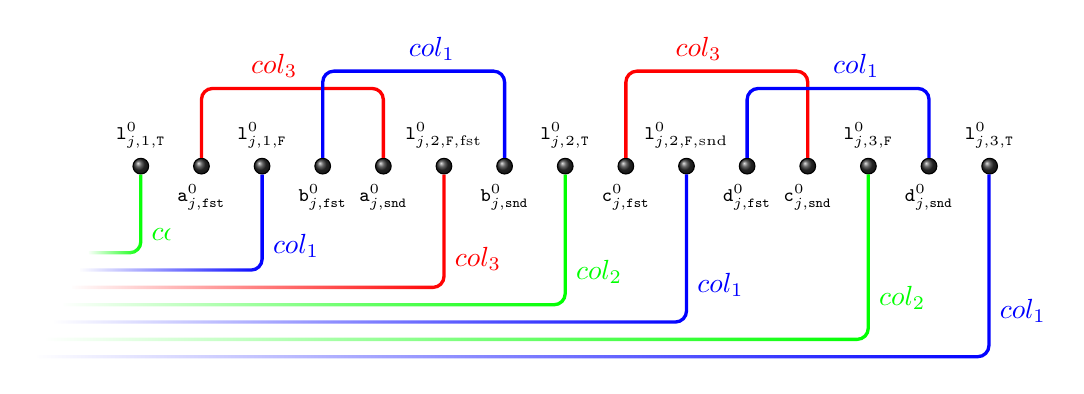
\begin{tikzpicture}
      [
      scale=.22,,,
      my vertex/.style={basic vertex,
      minimum size=1pt,
      inner sep=2pt,
      ball color=black!80},
      ]

      % vertices
      \foreach \i/\o/\l [evaluate=\i as \x using \i*3.5] in
      {
      1/above/\texttt{l}^0_{j,1,\TRUE},
      2/below/\texttt{a}^0_{j,\LEFT},
      3/above/\texttt{l}^0_{j,1,\FALSE},
      4/below/\texttt{b}^0_{j,\LEFT},
      5/below/\texttt{a}^0_{j,\RIGHT},
      6/above/\texttt{l}^0_{j,2,\FALSE,\FST},
      7/below/\texttt{b}^0_{j,\RIGHT},
      8/above/\texttt{l}^0_{j,2,\TRUE},
      9/below/\texttt{c}^0_{j,\LEFT},
      10/above/\texttt{l}^0_{j,2,\FALSE,\SND},
      11/below/\texttt{d}^0_{j,\LEFT},
      12/below/\texttt{c}^0_{j,\RIGHT},
      13/above/\texttt{l}^0_{j,3,\FALSE},
      14/below/\texttt{d}^0_{j,\RIGHT},
      15/above/\texttt{l}^0_{j,3,\TRUE}
      }
      {
      \node [my vertex,label=\o:{\scriptsize $\l$}] (V\i) at (\x,0) {};
      }

      % edges
      \path [edge,color=red] (V2.north) -- ++ (0,4) --
      ($(V5.north)+(0,4)$) node [pos=0.4,above] {$\COLOR_3$}   -- (V5.north);

      \path [edge,color=blue] (V4.north) -- ++ (0,5) --
      ($(V7.north)+(0,5)$) node [pos=0.6,above] {$\COLOR_1$} -- (V7.north);

      \path [edge,color=red] (V9.north) -- ++ (0,5) --
      ($(V12.north)+(0,5)$) node [pos=0.4,above] {$\COLOR_3$} -- (V12.north);

      \path [edge,color=blue] (V11.north) -- ++ (0,4) --
      ($(V14.north)+(0,4)$) node [pos=0.6,above] {$\COLOR_1$} -- (V14.north);

      % incoming edges
      \draw [edge,color=green,path fading=west] (V1) -- node [pos=0.75,anchor=west] {$\COLOR_2$}
      ++(0,-5) -- +(-3,0) node {};

      \draw [edge,color=blue,path fading=west] (V3) -- node [pos=0.75,anchor=west] {$\COLOR_1$}
      ++(0,-6) -- +(-10.5,0) node {};

      \draw [edge,color=red,path fading=west] (V6)  -- node [pos=0.75,anchor=west] {$\COLOR_3$}
      ++(0,-7)  -- +(-21.5,0) node {};

      \draw [edge,color=green,path fading=west] (V8)  -- node [pos=0.75,anchor=west] {$\COLOR_2$}
      ++(0,-8)  -- +(-29,0) node {};

      \draw [edge,color=blue,path fading=west] (V10) -- node [pos=0.75,anchor=west] {$\COLOR_1$}
      ++(0,-9) -- +(-36.5,0) node {};

      \draw [edge,color=green,path fading=west] (V13) -- node [pos=0.75,anchor=west] {$\COLOR_2$}
      ++(0,-10) -- +(-47.5,0) node {};

      \draw [edge,color=blue,path fading=west] (V15) -- node [pos=0.75,anchor=west] {$\COLOR_1$}
      ++(0,-11) -- +(-55,0) node {};

      %\node [text width=2.5cm,anchor=west] at (-15.5,-8.5) {\scriptsize Towards the variable gadgets};

    \end{tikzpicture}
    \caption{%
    Clause gadget $\texttt{Cls}^{0}_{j}$ for clause $(\ell_{j,1} \vee \ell_{j,2} \vee \ell_{j,3})$
    in case the literals $\ell_{j,1}$, $\ell_{j,2}$ and $\ell_{j,3}$ evaluate to false, false and true,
    respectivelly, according to the satisfying assignment $f$.
    }% end caption  \end{subfigure}
  \end{subfigure}

  \vspace{.5cm}

  \begin{subfigure}[b]{\textwidth}
    \centering
    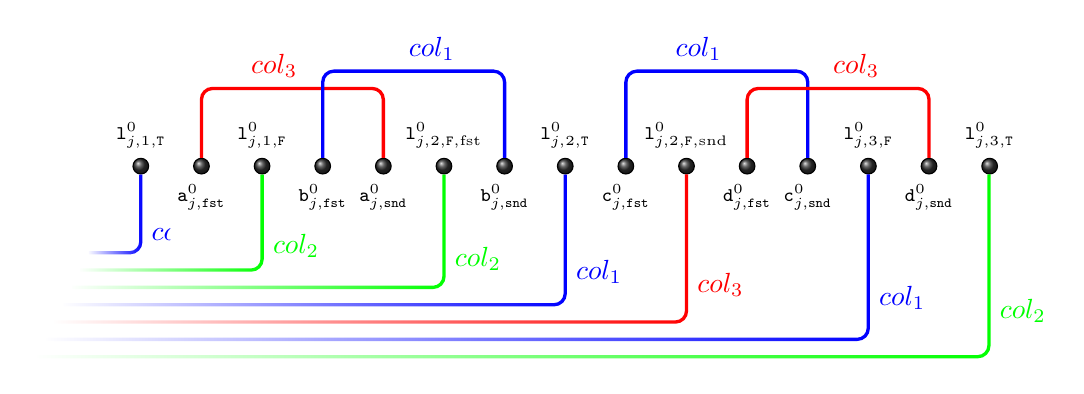
\begin{tikzpicture}
      [
      scale=.22,,,
      my vertex/.style={basic vertex,
      minimum size=1pt,
      inner sep=2pt,
      ball color=black!80},
      ]

      % vertices
      \foreach \i/\o/\l [evaluate=\i as \x using \i*3.5] in
      {
      1/above/\texttt{l}^0_{j,1,\TRUE},
      2/below/\texttt{a}^0_{j,\LEFT},
      3/above/\texttt{l}^0_{j,1,\FALSE},
      4/below/\texttt{b}^0_{j,\LEFT},
      5/below/\texttt{a}^0_{j,\RIGHT},
      6/above/\texttt{l}^0_{j,2,\FALSE,\FST},
      7/below/\texttt{b}^0_{j,\RIGHT},
      8/above/\texttt{l}^0_{j,2,\TRUE},
      9/below/\texttt{c}^0_{j,\LEFT},
      10/above/\texttt{l}^0_{j,2,\FALSE,\SND},
      11/below/\texttt{d}^0_{j,\LEFT},
      12/below/\texttt{c}^0_{j,\RIGHT},
      13/above/\texttt{l}^0_{j,3,\FALSE},
      14/below/\texttt{d}^0_{j,\RIGHT},
      15/above/\texttt{l}^0_{j,3,\TRUE}
      }
      {
      \node [my vertex,label=\o:{\scriptsize $\l$}] (V\i) at (\x,0) {};
      }

      % edges
      \path [edge,color=red] (V2.north) -- ++ (0,4) --
      ($(V5.north)+(0,4)$) node [pos=0.4,above] {$\COLOR_3$} -- (V5.north);

      \path [edge,color=blue] (V4.north) -- ++ (0,5) --
      ($(V7.north)+(0,5)$) node [pos=0.6,above] {$\COLOR_1$} -- (V7.north);

      \path [edge,color=blue] (V9.north) -- ++ (0,5) --
      ($(V12.north)+(0,5)$) node [pos=0.4,above] {$\COLOR_1$} -- (V12.north);

      \path [edge,color=red] (V11.north) -- ++ (0,4) --
      ($(V14.north)+(0,4)$) node [pos=0.6,above] {$\COLOR_3$} -- (V14.north);

      % incoming edges
      \draw [edge,color=blue,path fading=west] (V1) -- node [pos=0.75,anchor=west] {$\COLOR_1$}
      ++(0,-5) -- +(-3,0) node {};

      \draw [edge,color=green,path fading=west] (V3) -- node [pos=0.75,anchor=west] {$\COLOR_2$}
      ++(0,-6) -- +(-10.5,0) node {};

      \draw [edge,color=green,path fading=west] (V6)  -- node [pos=0.75,anchor=west] {$\COLOR_2$}
      ++(0,-7)  -- +(-21.5,0) node {};

      \draw [edge,color=blue,path fading=west] (V8)  -- node [pos=0.75,anchor=west] {$\COLOR_1$}
      ++(0,-8)  -- +(-29,0) node {};

      \draw [edge,color=red,path fading=west] (V10) --  node [pos=0.75,anchor=west] {$\COLOR_3$}
      ++(0,-9) -- +(-36.5,0) node {};

      \draw [edge,color=blue,path fading=west] (V13) -- node [pos=0.75,anchor=west] {$\COLOR_1$}
      ++(0,-10) -- +(-47.5,0) node {};

      \draw [edge,color=green,path fading=west] (V15) -- node [pos=0.75,anchor=west] {$\COLOR_2$}
      ++(0,-11) -- +(-55,0) node {};

      %\node [text width=2.5cm,anchor=west] at (-15.5,-8.5) {\scriptsize Towards the variable gadgets};

    \end{tikzpicture}
    \caption{%
    Clause gadget $\texttt{Cls}^{0}_{j}$ for clause $(\ell_{j,1} \vee \ell_{j,2} \vee \ell_{j,3})$
    in case the literals $\ell_{j,1}$, $\ell_{j,2}$ and $\ell_{j,3}$ evaluate to true, true and false,
    respectivelly, according to the satisfying assignment $f$.
    }% end caption  \end{subfigure}
  \end{subfigure}

\end{figure}

\begin{figure}\ContinuedFloat

  \begin{subfigure}[b]{\textwidth}
    \centering
    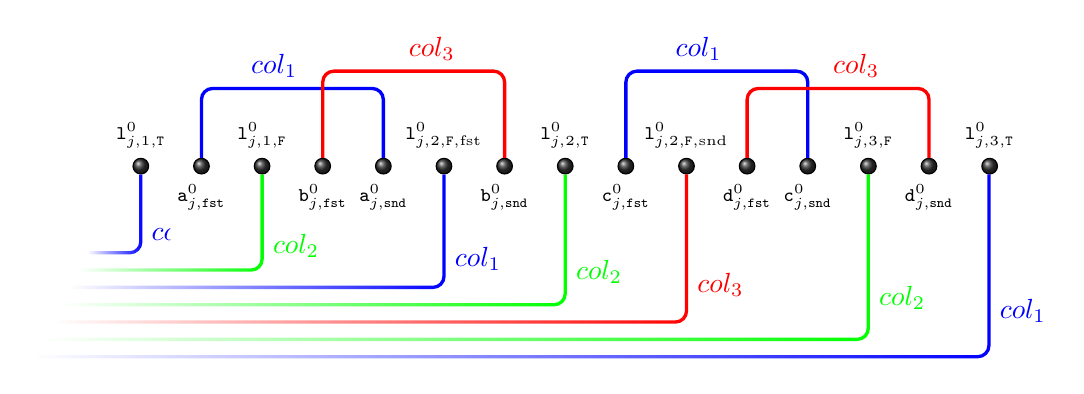
\begin{tikzpicture}
      [
      scale=.22,,,
      my vertex/.style={basic vertex,
      minimum size=1pt,
      inner sep=2pt,
      ball color=black!80},
      ]

      % vertices
      \foreach \i/\o/\l [evaluate=\i as \x using \i*3.5] in
      {
      1/above/\texttt{l}^0_{j,1,\TRUE},
      2/below/\texttt{a}^0_{j,\LEFT},
      3/above/\texttt{l}^0_{j,1,\FALSE},
      4/below/\texttt{b}^0_{j,\LEFT},
      5/below/\texttt{a}^0_{j,\RIGHT},
      6/above/\texttt{l}^0_{j,2,\FALSE,\FST},
      7/below/\texttt{b}^0_{j,\RIGHT},
      8/above/\texttt{l}^0_{j,2,\TRUE},
      9/below/\texttt{c}^0_{j,\LEFT},
      10/above/\texttt{l}^0_{j,2,\FALSE,\SND},
      11/below/\texttt{d}^0_{j,\LEFT},
      12/below/\texttt{c}^0_{j,\RIGHT},
      13/above/\texttt{l}^0_{j,3,\FALSE},
      14/below/\texttt{d}^0_{j,\RIGHT},
      15/above/\texttt{l}^0_{j,3,\TRUE}
      }
      {
      \node [my vertex,label=\o:{\scriptsize $\l$}] (V\i) at (\x,0) {};
      }

      % edges
      \path [edge,color=blue] (V2.north) -- ++ (0,4) --
      ($(V5.north)+(0,4)$) node [pos=0.4,above] {$\COLOR_1$} -- (V5.north);

      \path [edge,color=red] (V4.north) -- ++ (0,5) --
      ($(V7.north)+(0,5)$) node [pos=0.6,above] {$\COLOR_3$} -- (V7.north);

      \path [edge,color=blue] (V9.north) -- ++ (0,5) --
      ($(V12.north)+(0,5)$) node [pos=0.4,above] {$\COLOR_1$} -- (V12.north);

      \path [edge,color=red] (V11.north) -- ++ (0,4) --
      ($(V14.north)+(0,4)$) node [pos=0.6,above] {$\COLOR_3$} -- (V14.north);

      % incoming edges
      \draw [edge,color=blue,path fading=west] (V1) -- node [pos=0.75,anchor=west] {$\COLOR_1$}
      ++(0,-5) -- +(-3,0) node {};

      \draw [edge,color=green,path fading=west] (V3) -- node [pos=0.75,anchor=west] {$\COLOR_2$}
      ++(0,-6) -- +(-10.5,0) node {};

      \draw [edge,color=blue,path fading=west] (V6)  -- node [pos=0.75,anchor=west] {$\COLOR_1$}
      ++(0,-7)  -- +(-21.5,0) node {};

      \draw [edge,color=green,path fading=west] (V8)  -- node [pos=0.75,anchor=west] {$\COLOR_2$}
      ++(0,-8)  -- +(-29,0) node {};

      \draw [edge,color=red,path fading=west] (V10) -- node [pos=0.75,anchor=west] {$\COLOR_3$}
      ++(0,-9) -- +(-36.5,0) node {};

      \draw [edge,color=green,path fading=west] (V13) -- node [pos=0.75,anchor=west] {$\COLOR_2$}
      ++(0,-10) -- +(-47.5,0) node {};

      \draw [edge,color=blue,path fading=west] (V15) -- node [pos=0.75,anchor=west] {$\COLOR_1$}
      ++(0,-11) -- +(-55,0) node {};

      %\node [text width=2.5cm,anchor=west] at (-15.5,-8.5) {\scriptsize Towards the variable gadgets};

    \end{tikzpicture}
    \caption{%
    Clause gadget $\texttt{Cls}^{0}_{j}$ for clause $(\ell_{j,1} \vee \ell_{j,2} \vee \ell_{j,3})$
    in case the literals $\ell_{j,1}$, $\ell_{j,2}$ and $\ell_{j,3}$ evaluate to true, false and true,
    respectivelly, according to the satisfying assignment $f$.
    }% end caption
  \end{subfigure}

  \vspace{.5cm}

  \centering
  \begin{subfigure}[b]{\textwidth}
    \centering
    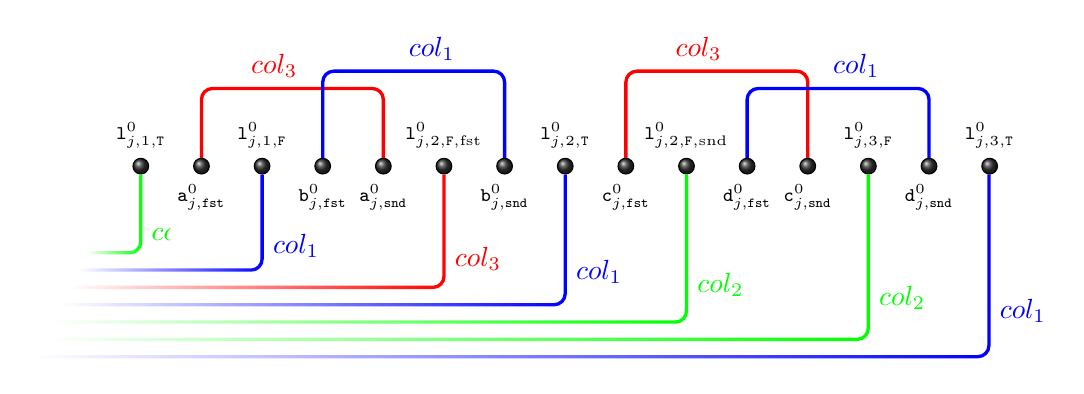
\begin{tikzpicture}
      [
      scale=.22,,,
      my vertex/.style={basic vertex,
      minimum size=1pt,
      inner sep=2pt,
      ball color=black!80},
      ]

      % vertices
      \foreach \i/\o/\l [evaluate=\i as \x using \i*3.5] in
      {
      1/above/\texttt{l}^0_{j,1,\TRUE},
      2/below/\texttt{a}^0_{j,\LEFT},
      3/above/\texttt{l}^0_{j,1,\FALSE},
      4/below/\texttt{b}^0_{j,\LEFT},
      5/below/\texttt{a}^0_{j,\RIGHT},
      6/above/\texttt{l}^0_{j,2,\FALSE,\FST},
      7/below/\texttt{b}^0_{j,\RIGHT},
      8/above/\texttt{l}^0_{j,2,\TRUE},
      9/below/\texttt{c}^0_{j,\LEFT},
      10/above/\texttt{l}^0_{j,2,\FALSE,\SND},
      11/below/\texttt{d}^0_{j,\LEFT},
      12/below/\texttt{c}^0_{j,\RIGHT},
      13/above/\texttt{l}^0_{j,3,\FALSE},
      14/below/\texttt{d}^0_{j,\RIGHT},
      15/above/\texttt{l}^0_{j,3,\TRUE}
      }
      {
      \node [my vertex,label=\o:{\scriptsize $\l$}] (V\i) at (\x,0) {};
      }

      % edges
      \path [edge,color=red] (V2.north) -- ++ (0,4) --
      ($(V5.north)+(0,4)$) node [pos=0.4,above] {$\COLOR_3$} -- (V5.north);

      \path [edge,color=blue] (V4.north) -- ++ (0,5) --
      ($(V7.north)+(0,5)$) node [pos=0.6,above] {$\COLOR_1$} -- (V7.north);

      \path [edge,color=red] (V9.north) -- ++ (0,5) --
      ($(V12.north)+(0,5)$) node [pos=0.4,above] {$\COLOR_3$} -- (V12.north);

      \path [edge,color=blue] (V11.north) -- ++ (0,4) --
      ($(V14.north)+(0,4)$) node [pos=0.6,above] {$\COLOR_1$} -- (V14.north);

      % incoming edges
      \draw [edge,color=green,path fading=west] (V1) -- node [pos=0.75,anchor=west] {$\COLOR_2$}
      ++(0,-5) -- +(-3,0) node {};

      \draw [edge,color=blue,path fading=west] (V3) -- node [pos=0.75,anchor=west] {$\COLOR_1$}
      ++(0,-6) -- +(-10.5,0) node {};

      \draw [edge,color=red,path fading=west] (V6)  -- node [pos=0.75,anchor=west] {$\COLOR_3$}
      ++(0,-7)  -- +(-21.5,0) node {};

      \draw [edge,color=blue,path fading=west] (V8)  -- node [pos=0.75,anchor=west] {$\COLOR_1$}
      ++(0,-8)  -- +(-29,0) node {};

      \draw [edge,color=green,path fading=west] (V10) -- node [pos=0.75,anchor=west] {$\COLOR_2$}
      ++(0,-9) -- +(-36.5,0) node {};

      \draw [edge,color=green,path fading=west] (V13) -- node [pos=0.75,anchor=west] {$\COLOR_2$}
      ++(0,-10) -- +(-47.5,0) node {};

      \draw [edge,color=blue,path fading=west] (V15) -- node [pos=0.75,anchor=west] {$\COLOR_1$}
      ++(0,-11) -- +(-55,0) node {};

      %\node [text width=2.5cm,anchor=west] at (-15.5,-8.5) {\scriptsize Towards the variable gadgets};

    \end{tikzpicture}
    \caption{%
    Clause gadget $\texttt{Cls}^{0}_{j}$ for clause $(\ell_{j,1} \vee \ell_{j,2} \vee \ell_{j,3})$
    in case the literals $\ell_{j,1}$, $\ell_{j,2}$ and $\ell_{j,3}$ evaluate to false, true and true,
    respectivelly, according to the satisfying assignment $f$.
    }% end caption
  \end{subfigure}

  \vspace{.5cm}

  \begin{subfigure}[b]{\textwidth}
    \centering
    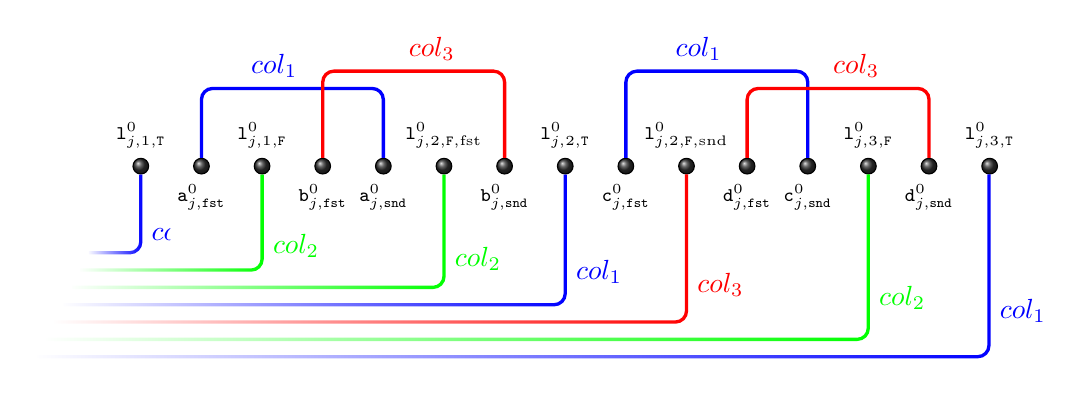
\begin{tikzpicture}
      [
      scale=.22,,,
      my vertex/.style={basic vertex,
      minimum size=1pt,
      inner sep=2pt,
      ball color=black!80},
      ]

      % vertices
      \foreach \i/\o/\l [evaluate=\i as \x using \i*3.5] in
      {
      1/above/\texttt{l}^0_{j,1,\TRUE},
      2/below/\texttt{a}^0_{j,\LEFT},
      3/above/\texttt{l}^0_{j,1,\FALSE},
      4/below/\texttt{b}^0_{j,\LEFT},
      5/below/\texttt{a}^0_{j,\RIGHT},
      6/above/\texttt{l}^0_{j,2,\FALSE,\FST},
      7/below/\texttt{b}^0_{j,\RIGHT},
      8/above/\texttt{l}^0_{j,2,\TRUE},
      9/below/\texttt{c}^0_{j,\LEFT},
      10/above/\texttt{l}^0_{j,2,\FALSE,\SND},
      11/below/\texttt{d}^0_{j,\LEFT},
      12/below/\texttt{c}^0_{j,\RIGHT},
      13/above/\texttt{l}^0_{j,3,\FALSE},
      14/below/\texttt{d}^0_{j,\RIGHT},
      15/above/\texttt{l}^0_{j,3,\TRUE}
      }
      {
      \node [my vertex,label=\o:{\scriptsize $\l$}] (V\i) at (\x,0) {};
      }

      % edges
      \path [edge,color=blue] (V2.north) -- ++ (0,4) --
      ($(V5.north)+(0,4)$) node [pos=0.4,above] {$\COLOR_1$} -- (V5.north);

      \path [edge,color=red] (V4.north) -- ++ (0,5) --
      ($(V7.north)+(0,5)$) node [pos=0.6,above] {$\COLOR_3$} -- (V7.north);

      \path [edge,color=blue] (V9.north) -- ++ (0,5) --
      ($(V12.north)+(0,5)$) node [pos=0.4,above] {$\COLOR_1$} -- (V12.north);

      \path [edge,color=red] (V11.north) -- ++ (0,4) --
      ($(V14.north)+(0,4)$) node [pos=0.6,above] {$\COLOR_3$} -- (V14.north);

      % incoming edges
      \draw [edge,color=blue,path fading=west] (V1) -- node [pos=0.75,anchor=west] {$\COLOR_1$}
      ++(0,-5) -- +(-3,0) node {};

      \draw [edge,color=green,path fading=west] (V3) -- node [pos=0.75,anchor=west] {$\COLOR_2$}
      ++(0,-6) -- +(-10.5,0) node {};

      \draw [edge,color=green,path fading=west] (V6)  -- node [pos=0.75,anchor=west] {$\COLOR_2$}
      ++(0,-7)  -- +(-21.5,0) node {};

      \draw [edge,color=blue,path fading=west] (V8)  -- node [pos=0.75,anchor=west] {$\COLOR_1$}
       ++(0,-8)  -- +(-29,0) node {};

      \draw [edge,color=red,path fading=west] (V10) -- node [pos=0.75,anchor=west] {$\COLOR_3$}
      ++(0,-9) -- +(-36.5,0) node {};

      \draw [edge,color=green,path fading=west] (V13) -- node [pos=0.75,anchor=west] {$\COLOR_2$}
      ++(0,-10) -- +(-47.5,0) node {};

      \draw [edge,color=blue,path fading=west] (V15) -- node [pos=0.75,anchor=west] {$\COLOR_1$}
      ++(0,-11) -- +(-55,0) node {};

      %\node [text width=2.5cm,anchor=west] at (-15.5,-8.5) {\scriptsize Towards the variable gadgets};

    \end{tikzpicture}
    \caption{%
    Clause gadget $\texttt{Cls}^{0}_{j}$ for clause $(\ell_{j,1} \vee \ell_{j,2} \vee \ell_{j,3})$
    in case the literals $\ell_{j,1}$, $\ell_{j,2}$ and $\ell_{j,3}$ evaluate to true, true and true,
    respectivelly, according to the satisfying assignment $f$.
    }% end caption
  \end{subfigure}
  \caption{The general caption.}
\end{figure}



\end{proof}


% Permutation coloring
\section{Permutation coloring}
\label{section:Permutation coloring}

We are back to coloring permutations. We show how to transform
linear graph colorings to permutation colorings.
We need a new definition.
Let $G = (V, E)$ be a linear graph. For any two connected vertices
$v_i, v_j \in V$, $i < j$ or $j < i$,
we define
$$
\RANK(v_i, v_j) = \left|\left\{v_k \in V : \{v_i, v_k\} \in E \text{ and } k \leq j\right\}\right|.
$$
In other words, $\RANK(v_i, v_j) = k+1$ if there exist exactly $k$ vertices
$v_{i_1}, v_{i_2}, \dots, v_{i_k} \in N(v_i)$
with $\max \{i_1, i_2, \dots, i_k\} < j$.

\begin{proposition}
  \label{proposition:3-permutation coloring is NP-complete}
  \textsc{$3$-permutation coloring} is \NP-complete.
\end{proposition}

\begin{proof}
  We reduce from \textsc{$k$-Linear Graph Coloring} (Proposition~\ref{proposition:3-Linear Graph Coloring is NP-complete}).
  Let $(G^{0} \,|\, G^{1}, G^{2}, \dots, G^{k})$ be an arbitrary instance of \textsc{$k$-Linear Graph Coloring}.
  Write $G^{i} = (V^i, E^i)$,
  $n_i = |V^i|$ $m_i = |E^i|$ for $0 \leq i \leq k$.
  We show how to construct an instance
  $(\pi | \sigma_1, \sigma_2, \dots, \sigma_k)$ of
  \textsc{$k$-permutation coloring}.

  Define $N_i = 2n_i + 4m_i + 1$ for $0 \leq i \leq k$.
  We first associate the permutation $\pi$ to the linear graph $G^{0}$.
  Write $V^0 = \{v^0_i : 1 \leq i \leq n_0\}$ and
  $E^0 = \{e^0_i : 1 \leq i \leq m_0\}$.
  Define the permutations
  \begin{align*}
    \pi(V)
    &=
    \left(\bigoplus_{i=1}^{n_0} (d(v^0_i)+2) \; 1\right) [2m_0+2kN_0]
    \\
    \pi(E)
    &=
    \bigoplus_{j=1}^{m_0} 2 \; f^0(e^0_j) \; g^0(e^0_j) \; 1
    \\
    \pi(\text{Sep}_1)
    &=
    \left(\bigominus_{i=1}^{k} \mathbf{\nearrow}_{N_0}\right) [2n]
    \\
    \pi(\text{Sep}_2)
    &=
    \left(\bigominus_{i=1}^{k} \mathbf{\nearrow}_{N_0}\right) [2n+kN]
    \\
    \intertext{where $f : E^0 \to \mathbb{N}$ and $g : E^0 \to \mathbb{N}$
    are defined as follows}
    \forall e^0_j = (v^0_p, v^0_q) \in E_0,\quad f^0(e^0_j)
    &=
    2m_0 + 2kN_0 + \sum_{j=1}^{p-1}\left(2+d(v^0_j)\right) + \RANK\left(v^0_p, v^0_q\right)
    \\
    \forall e^0_j = (v^0_p, v^0_q) \in E_0,\quad g^0(e^0_j)
    &=
    2m_0 + 2kN_0 + \sum_{j=1}^{q-1}\left(2+d(v^0_j)\right) + \RANK\left(v^0_q, v^0_p\right)\text{.}
    \end{align*}

    In other words,
    $\pi(V)$ is the direct sum of $n_0$ decreasing permutations
    that are all order-isomorphic to $21$,
    $\pi(E)$ is the direct sum of $m_0$ permutations that are all
    order-isomorphic to $2341$ (since $2 < f(e^0_i) < g(e^0_i)$
    for $1 \leq i \leq m_0$), and
    both $\pi(\text{Sep}_1)$ and $\pi(\text{Sep}_2)$ are the skew sums
    of $k$ permutations that are all order isomorphic to $12 \dots k$.
    Finally, we obtain the target permutation $\pi$ by gathering the parts
    $\pi(V)$, $\pi(\text{Sep}_1)$, $\pi(E)$ and $\pi(\text{Sep}_2)$:
    $$
      \pi =
      \pi(V)   \;
      \pi(\text{Sep}_1) \;
      \pi(E)   \;
      \pi(\text{Sep}_2)\text{.}
    $$


  \begin{figure}[htbp!]
  \centering
  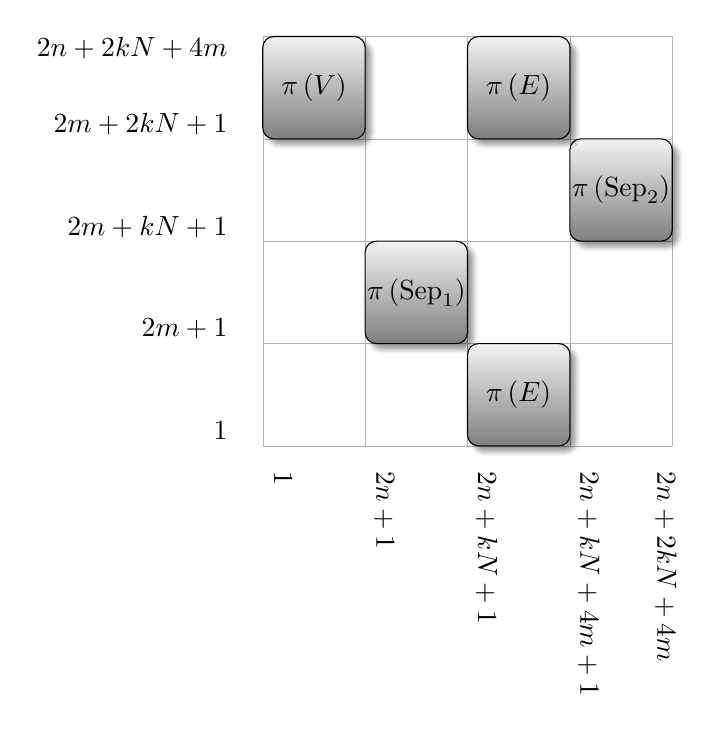
\begin{tikzpicture}
  [
    scale=.65,
    box/.style={
      shade,
      blur shadow={shadow blur steps=5,shadow blur extra rounding=1.3pt},
      top color=black!5,
      bottom color=black!50
    },
    gadget/.style={
      box,
      rounded corners
    },
    r/.style={
      box,
      draw,
      ultra thick,
    }
  ]
  \draw [help lines,step=2cm,black!30,fill=black!10] (0,0) grid (8,8);
  \draw [gadget] (0,6) rectangle ++(2,2);
  \node [] at (1,7) {$\pi\left(V\right)$};
  \draw [gadget] (2,2) rectangle ++(2,2);
  \node [] at (3,3) {$\pi\left(\text{Sep}_1\right)$};
  \draw [gadget] (4,0) rectangle ++(2,2);
  \node [] at (5,1) {$\pi\left(E\right)$};
  \draw [gadget] (6,4) rectangle ++(2,2);
  \node [] at (7,5) {$\pi\left(\text{Sep}_2\right)$};
  \draw [gadget] (4,6) rectangle ++(2,2);
  \node [] at (5,7) {$\pi\left(E\right)$};
    % labels
    % x-labels
    \node [label={[text depth=1.75ex,label distance=0.2cm,rotate=-90]right:{$1$}}] at (0,0) {};
    % \node [label={[text depth=1.75ex,label distance=0.2cm,rotate=-90]right:{$2n$}}] at (1.5,0) {};
    \node [label={[text depth=1.75ex,label distance=0.2cm,rotate=-90]right:{$2n+1$}}] at (2,0) {};
    % \node [label={[text depth=1.75ex,label distance=0.2cm,rotate=-90]right:{$2n+kN$}}] at (3.5,0) {};
    \node [label={[text depth=1.75ex,label distance=0.2cm,rotate=-90]right:{$2n+kN+1$}}] at (4,0) {};
    % \node [label={[text depth=1.75ex,label distance=0.2cm,rotate=-90]right:{$2n+kN+4m$}}] at (5.5,0) {};
    \node [label={[text depth=1.75ex,label distance=0.2cm,rotate=-90]right:{$2n+kN+4m+1$}}] at (6,0) {};
    \node [label={[text depth=1.75ex,label distance=0.2cm,rotate=-90]right:{$2n+2kN+4m$}}] at (7.5,0) {};
    % y-labels
    \node [label={[text depth=1.75ex,label distance=0.2cm]left:{$1$}}] at (0,0.1) {};
    % \node [label={[text depth=1.75ex,label distance=0.2cm]left:{$2m2$}}] at (0,1.6) {};
    \node [label={[text depth=1.75ex,label distance=0.2cm]left:{$2m+1$}}] at (0,2.1) {};
    % \node [label={[text depth=1.75ex,label distance=0.2cm]left:{$2m+kN$}}] at (0,3.6) {};
    \node [label={[text depth=1.75ex,label distance=0.2cm]left:{$2m+kN+1$}}] at (0,4.1) {};
    % \node [label={[text depth=1.75ex,label distance=0.2cm]left:{$2m+2kN$}}] at (0,5.6) {};
    \node [label={[text depth=1.75ex,label distance=0.2cm]left:{$2m+2kN+1$}}] at (0,6.1) {};
    \node [label={[text depth=1.75ex,label distance=0.2cm]left:{$2n+2kN+4m$}}] at (0,7.6) {};
  \end{tikzpicture}
  \caption{\label{fig:NP2:bird eye view pi}%
    Bird's-eye view of the permutation $\pi$.
  }% end caption
\end{figure}

  
\begin{figure}
  \centering
  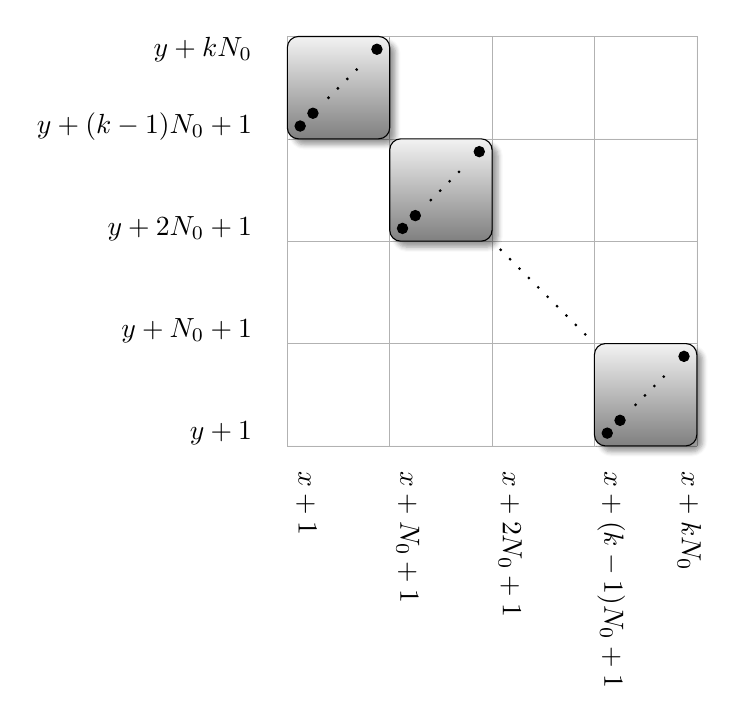
\begin{tikzpicture}
  [
    scale=.65,
    box/.style={
      shade,
      blur shadow={shadow blur steps=5,shadow blur extra rounding=1.3pt},
      top color=black!5,
      bottom color=black!50
    },
    monotone/.style={>=stealth',->,thick,shorten >=.5pt,shorten <=3pt},
  ]
    % separator gadgets
    % monotonic sequences
    \draw [help lines,step=2cm,black!30,fill=black!10] (0,0) grid (8,8);
    % I_1
    \draw [box,rounded corners] (0,6) rectangle ++(2,2);
    \foreach \x/\y in {0.25/6.25,0.5/6.5,1.75/7.75}
      \draw [fill=black] (\x,\y) circle (0.1);
    \draw [thick,loosely dotted,thick,shorten >=1pt,shorten <=1pt] (.75,6.75) -- (1.5,7.5);
    % I_2
    \draw [box,rounded corners] (2,4) rectangle ++(2,2);
    \foreach \x/\y in {2.25/4.25,2.5/4.5,3.75/5.75}
      \draw [fill=black] (\x,\y) circle (0.1);
    \draw [thick,loosely dotted,thick,shorten >=1pt,shorten <=1pt] (2.75,4.75) -- (3.5,5.5);
    % again and angain
    \draw [thick,loosely dotted,thick,shorten >=4pt,shorten <=4pt] (4,4) -- (6,2);
    % I_k
    \draw [box,rounded corners] (6,0) rectangle ++(2,2);
    \foreach \x/\y in {6.25/.25,6.5/.5,7.75/1.75}
      \draw [fill=black] (\x,\y) circle (0.1);
    \draw [thick,loosely dotted,thick,shorten >=1pt,shorten <=1pt] (6.75,.75) -- (7.5,1.5);
    % labels
    % x-labels
    \node [label={[text depth=1.75ex,label distance=0.2cm,rotate=-90]right:{$x+1$}}] at (0,0) {};
    % \node [label={[text depth=1.75ex,label distance=0.2cm,rotate=-90]right:{$x+N_0$}}] at (1.5,0) {};
    \node [label={[text depth=1.75ex,label distance=0.2cm,rotate=-90]right:{$x+N_0+1$}}] at (2,0) {};
    % \node [label={[text depth=1.75ex,label distance=0.2cm,rotate=-90]right:{$x+2N_0$}}] at (3.5,0) {};
    \node [label={[text depth=1.75ex,label distance=0.2cm,rotate=-90]right:{$x+2N_0+1$}}] at (4,0) {};
    % \node [label={[text depth=1.75ex,label distance=0.2cm,rotate=-90]right:{$x+(k-1)N_0$}}] at (5.5,0) {};
    \node [label={[text depth=1.75ex,label distance=0.2cm,rotate=-90]right:{$x+(k-1)N_0+1$}}] at (6,0) {};
    \node [label={[text depth=1.75ex,label distance=0.2cm,rotate=-90]right:{$x+kN_0$}}] at (7.5,0) {};
    % y-labels
    \node [label={[text depth=1.75ex,label distance=0.2cm]left:{$y+1$}}] at (0,0.1) {};
    % \node [label={[text depth=1.75ex,label distance=0.2cm]left:{$y+N_0$}}] at (0,1.6) {};
    \node [label={[text depth=1.75ex,label distance=0.2cm]left:{$y+N_0+1$}}] at (0,2.1) {};
    % \node [label={[text depth=1.75ex,label distance=0.2cm]left:{$y+2N_0$}}] at (0,3.6) {};
    \node [label={[text depth=1.75ex,label distance=0.2cm]left:{$y+2N_0+1$}}] at (0,4.1) {};
    % \node [label={[text depth=1.75ex,label distance=0.2cm]left:{$y+(k-1)N_0$}}] at (0,5.6) {};
    \node [label={[text depth=1.75ex,label distance=0.2cm]left:{$y+(k-1)N_0+1$}}] at (0,6.1) {};
    \node [label={[text depth=1.75ex,label distance=0.2cm]left:{$y+kN_0$}}] at (0,7.6) {};
  \end{tikzpicture}
  \caption{\label{fig:NP2:separators}%
    Schematic representation of $\pi(\text{Sep}_1)$ and $\pi(\text{Sep}_2)$,
    where the offsetis $O=2n$ for
    $\pi(\text{Sep}_1)$ and $O=2n+kN$ for $\pi(\text{Sep}_2)$.
  }% end caption
\end{figure}

  \begin{figure}
  \centering
  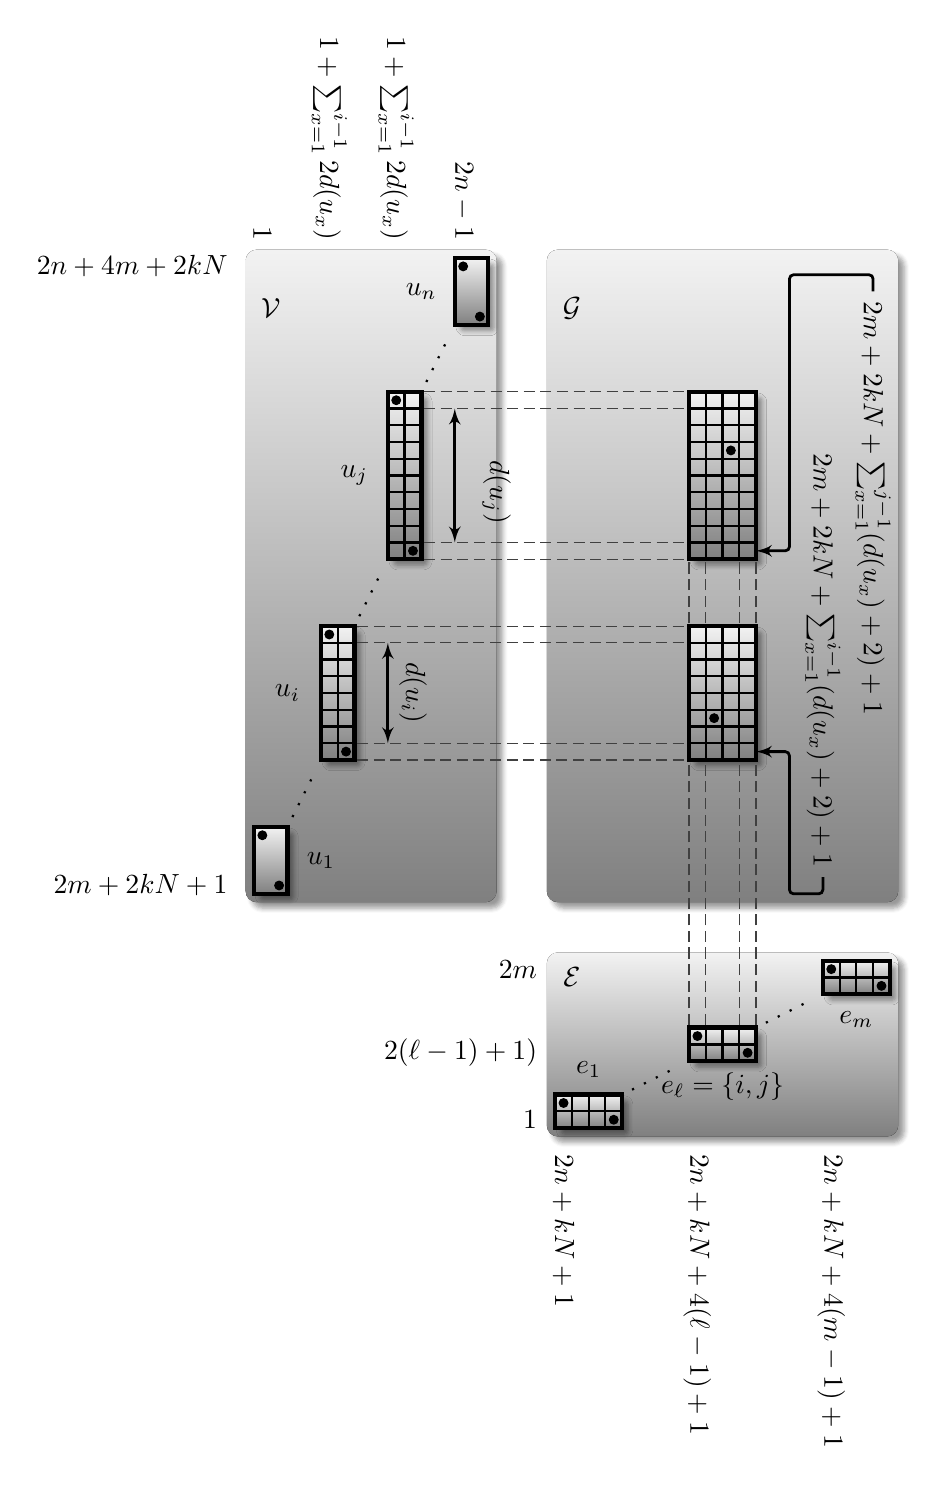
\begin{tikzpicture}
  [
    scale=.425,
    box/.style={
      shade,
      blur shadow={shadow blur steps=5,shadow blur extra rounding=1.3pt},
      top color=black!5,
      bottom color=black!50
    },
    gadget/.style={
      box,
      rounded corners
    },
    r/.style={
      box,
      draw,
      ultra thick,
    }
  ]
    % V gadget
    \fill [gadget] (-0.25,9.75) rectangle (7.25,29.25);
    \node at (0.5,27.5) {$\mathcal{V}$};
    % vertex 1
    \path [r] (0,10) -- ++(1,0) -- ++(0,2) -- ++(-1,0) -- cycle;
    \foreach \x/\y in {0.25/11.75,0.75/10.25}
      \draw [fill=black] (\x,\y) circle (0.13);
    \node at (2,11) {$u_1$};
    % again and again
    \draw [thick,loosely dotted,thick,shorten >=4pt,shorten <=4pt] (1,12) -- (2,14);
    % vertex i
    \path [r] (2,14) -- ++(1,0) -- ++(0,4) -- ++(-1,0) -- cycle;
    \draw [thick,step=0.5cm] (2,14) grid (3,18);
    \path [draw,ultra thick] (2,14) -- ++(1,0) -- ++(0,4) -- ++(-1,0) -- cycle;
    \foreach \x/\y in {2.25/17.75,2.75/14.25}
      \draw [fill=black] (\x,\y) circle (0.13);
    \node at (1,16) {$u_i$};
    % again and again
    \draw [thick,loosely dotted,thick,shorten >=4pt,shorten <=4pt] (3,18) -- (4,20);
    % vertex j
    \path [r] (4,20) -- ++(1,0) -- ++(0,5) -- ++(-1,0) -- cycle;
    \draw [thick,step=0.5cm] (4,20) grid (5,25);
    \path [draw,ultra thick] (4,20) -- ++(1,0) -- ++(0,5) -- ++(-1,0) -- cycle;
    \foreach \x/\y in {4.25/24.75,4.75/20.25}
      \draw [fill=black] (\x,\y) circle (0.13);
    \node at (3,22.5) {$u_j$};
    % again and again
    \draw [thick,loosely dotted,thick,shorten >=4pt,shorten <=4pt] (5,25) -- (6,27);
    % vertex n
    \path [r] (6,27) -- ++(1,0) -- ++(0,2) -- ++(-1,0) -- cycle;
    \foreach \x/\y in {6.25/28.75,6.75/27.25}
      \draw [fill=black] (\x,\y) circle (0.13);
    \node at (5,28) {$u_n$};

    % E gadget
    \fill [gadget] (8.75,2.75) rectangle (19.25,8.25);
    \node at (9.5,7.5) {$\mathcal{E}$};
    % first edge
    \path [r] (9,3) -- ++(2,0) -- ++(0,1) -- ++(-2,0) -- cycle;
    \draw [thick,step=0.5cm] (9,3) grid (11,4);
    \path [draw,ultra thick] (9,3) -- ++(2,0) -- ++(0,1) -- ++(-2,0) -- cycle;
    \foreach \x/\y in {9.25/3.75,10.75/3.25}
      \draw [fill=black] (\x,\y) circle (0.13);
    \node at (10,4.75) {$e_1$};
    % again and again
    \draw [thick,loosely dotted,thick,shorten >=4pt,shorten <=4pt] (11,4) -- (13,5);
    % edge (i,j))
    \path [r] (13,5) -- ++(2,0) -- ++(0,1) -- ++(-2,0) -- cycle;
    \draw [thick,step=0.5cm] (13,5) grid (15,6);
    \path [draw,ultra thick] (13,5) -- ++(2,0) -- ++(0,1) -- ++(-2,0) -- cycle;
    \foreach \x/\y in {13.25/5.75,14.75/5.25}
      \draw [fill=black] (\x,\y) circle (0.13);
    \node at (14,4.25) {$e_\ell = \{i,j\}$};
    % again and again
    \draw [thick,loosely dotted,thick,shorten >=4pt,shorten <=4pt] (15,6) -- (17,7);
    % last edge
    \path [r] (17,7) -- ++(2,0) -- ++(0,1) -- ++(-2,0) -- cycle;
    \draw [thick,step=0.5cm] (17,7) grid (19,8);
    \path [draw,ultra thick] (17,7) -- ++(2,0) -- ++(0,1) -- ++(-2,0) -- cycle;
    \foreach \x/\y in {17.25/7.75,18.75/7.25}
      \draw [fill=black] (\x,\y) circle (0.13);
    \node at (18,6.25) {$e_m$};

    % Connection gadget
    \fill [gadget] (8.75,9.75) rectangle (19.25,29.25);
    \node at (9.5,27.5) {$\mathcal{G}$};
    \fill [r] (13-0.001,14-0.001) rectangle (15,18);
    \draw [thick,step=0.5cm,black] (13-0.001,14-0.001) grid (15,18);
    \draw [fill=black] (13.75,15.25) circle (0.13);
    \fill [r] (13-0.001,20-0.001) rectangle (15,25);
    \draw [thick,step=0.5cm,black] (13-0.001,20-0.001) grid (15,25);
    \draw [fill=black] (14.25,23.25) circle (0.13);

    %  alignments
    % vertical
    \draw [black!75,dash pattern={on 4pt off 2pt},shorten >=1pt,shorten <=1pt] (13,6) -- (13,14);
    \draw [black!75,dash pattern={on 4pt off 2pt},shorten >=1pt,shorten <=1pt] (13,18) -- (13,20);
    \draw [black!75,dash pattern={on 4pt off 2pt},shorten >=1pt,shorten <=1pt] (15,6) -- (15,14);
    \draw [black!75,dash pattern={on 4pt off 2pt},shorten >=1pt,shorten <=1pt] (15,18) -- (15,20);
    %
    \draw [black!75,dash pattern={on 4pt off 2pt},shorten >=1pt,shorten <=1pt] (13.5,6) -- (13.5,14);
    \draw [black!75,dash pattern={on 4pt off 2pt},shorten >=1pt,shorten <=1pt] (13.5,18) -- (13.5,20);
    \draw [black!75,dash pattern={on 4pt off 2pt},shorten >=1pt,shorten <=1pt] (14.5,6) -- (14.5,14);
    \draw [black!75,dash pattern={on 4pt off 2pt},shorten >=1pt,shorten <=1pt] (14.5,18) -- (14.5,20);
    % horizontal
    \draw [black!75,dash pattern={on 4pt off 2pt},shorten >=1pt,shorten <=1pt] (3,14) -- (13,14);
    \draw [black!75,dash pattern={on 4pt off 2pt},shorten >=1pt,shorten <=1pt] (3,14.5) -- (13,14.5);
    \draw [black!75,dash pattern={on 4pt off 2pt},shorten >=1pt,shorten <=1pt] (3,17.5) -- (13,17.5);
    \draw [black!75,dash pattern={on 4pt off 2pt},shorten >=1pt,shorten <=1pt] (3,18) -- (13,18);
    \draw [black,line width=1pt,<->,>=latex'] (4,14.5) -- (4,17.5);
    \node [rotate=-90] at (4.75,16) {$d(u_i)$};
    \draw [black!75,dash pattern={on 4pt off 2pt},shorten >=1pt,shorten <=1pt] (5,20) -- (13,20);
    \draw [black!75,dash pattern={on 4pt off 2pt},shorten >=1pt,shorten <=1pt] (5,20.5) -- (13,20.5);
    \draw [black!75,dash pattern={on 4pt off 2pt},shorten >=1pt,shorten <=1pt] (5,24.5) -- (13,24.5);
    \draw [black!75,dash pattern={on 4pt off 2pt},shorten >=1pt,shorten <=1pt] (5,25) -- (13,25);
    \draw [black,line width=1pt,<->,>=latex'] (6,20.5) -- (6,24.5);
    \node [rotate=-90] at (7.25,22) {$d(u_j)$};

    % labels
    % vertex gadget
    % x-labels
    \node [anchor=east,rotate=-90] at (0.25,29.25) {$1$};
    \node [anchor=east,rotate=-90] at (2.25,29.25) {$1 + \sum_{x=1}^{i-1}2d(u_x)$};
    \node [anchor=east,rotate=-90] at (4.25,29.25) {$1 + \sum_{x=1}^{i-1}2d(u_x)$};
    \node [anchor=east,rotate=-90] at (6.25,29.25) {$2n-1$};
    % y-labels
    \node [anchor=east] at (-0.5,10.25) {$2m+2kN+1$};
    \node [anchor=east] at (-0.5,28.75) {$2n+4m+2kN$};
    % edge gadget
    % x-labels
    \node [rotate=-90,anchor=west] at (9.25,2.5) {$2n+kN+1$};
    \node [rotate=-90,anchor=west] at (13.25,2.5) {$2n+kN+4(\ell-1)+1$};
    \node [rotate=-90,anchor=west] at (17.25,2.5) {$2n+kN+4(m-1)+1$};
    % y-labels
    \node [anchor=east] at (8.75,3.25) {$1$};
    \node [anchor=east] at (8.75,5.25) {$2(\ell-1)+1)$};
    \node [anchor=east] at (8.75,7.75) {$2m$};
    % connection labels
    % y-labels
    \node [anchor=east,rotate=-90] at (17,10.5) {$2m+2kN+\sum_{x=1}^{i-1}(d(u_x)+2)+1$};
    \draw [black,line width=1pt,->,>=latex',rounded corners=1.5pt]
      (17,10.5) -- (17,10) -- (16,10) -- (16,14.25) -- (15,14.25);
    \node [anchor=west,rotate=-90] at (18.5,28) {$2m+2kN+\sum_{x=1}^{j-1}(d(u_x)+2)+1$};
    \draw [black,line width=1pt,->,>=latex',rounded corners=1.5pt]
      (18.5,28) -- (18.5,28.5) -- (16,28.5) -- (16,20.25) -- (15,20.25);
  \end{tikzpicture}
  \caption{\label{fig:NP2:connection zoom}%
  $\RANK(u_i, u_j) = 2$ and $\RANK(u_j, u_i) = 6 = d(u_j)$.
  }% end caption
\end{figure}


  A simplified representation of the permutation $\pi$ is given in
  Figure~\ref{fig:NP2:bird eye view pi}.
  A schematic representation of $\pi(\text{Sep}_1)$ and $\pi(\text{Sep}_2)$
  is given in Figure~\ref{fig:NP2:separators}, where the offset is $O=2n$ for
  $\pi(\text{Sep}_1)$ and $O=2n+kN$ for $\pi(\text{Sep}_2)$.
  A zoom of $\pi(E)$ is given in Figure~\ref{fig:NP2:connection zoom}.

  For example, referring Figure~\ref{fig:3-Linear-Graph Coloring} ($k=3$), we
  obtain from the linear graph $G^0$:
  $N_0 = 26 + 44 + 1 = 71$, $2m0+2kN_0= 22 + 426 = 448$, and hence
  $\pi(V) = \left(3 1 \oplus 3 1 \oplus 4 1 \oplus 4 1 \oplus 4 1 \oplus
  4 1 \oplus 4 1 \oplus 4 1 \oplus 4 1 \oplus 3 1 \oplus 3 1 \oplus 4 1 \oplus 3 1\right) [448]$,
  $\pi(E) = 2\;449\;479\;1 \oplus \dots$

  We now turn to associating the permutation $\sigma_i$, $1 \leq i \leq k$,
  to the linear graph $G^i = (V^i, E^i)$.
  The construction, as a whole, follows the same line as of $\pi$,
  the main difference being the \emph{separators}
  $\sigma_i\left(\text{Sep}_1\right)$ and
  $\sigma_i\left(\text{Sep}_2\right)$ that are both simplified.
  Define
  \begin{align*}
    \sigma_i(V)
    &=
    \left(\bigoplus_{j=1}^{n_i} (d(v^i_j)+2) \; 1\right) [2m_i+2N_i]
    \\
    \sigma_i(E)
    &=
    \bigoplus_{j=1}^{m_i} 2 \; f^i(e^0_j) \; g^i(e^0_j) \; 1
    \\
    \sigma_i\left(\text{Sep}_1\right)
    &=
    \mathbf{\nearrow}_{N_0} [2n_i]
    \\
    \sigma_i\left(\text{Sep}_2\right)
    &=
    \mathbf{\nearrow}_{N_0} [2n_i+N]
    \\
    \intertext{where $f^i : E^i \to \mathbb{N}$ and $g^i : E^i \to \mathbb{N}$
    are defined as follows}
    \forall e^i_j = (v^i_p, v^i_q) \in E_i,\quad f^i(e^0_j)
    &=
    2m_0 + 2kN_0 + \sum_{j=1}^{p-1}\left(2+d(v^0_j)\right) + \RANK\left(v^0_p, v^0_q\right)
    \\
    \forall e^i_j = (v^i_p, v^0_q) \in E_i,\quad g^i(e^0_j)
    &=
    2m_0 + 2kN_0 + \sum_{j=1}^{q-1}\left(2+d(v^0_j)\right) + \RANK\left(v^0_q, v^0_p\right)\text{.}
    \end{align*}
  %
  %   \intertext{where (assuming edge $e_{i,\ell} = (u_i, u_j)$)}
  %   x^1_{i,\ell}
  %   &=
  %   2m + 2kN + \sum_{\ell'=1}^{i-1}\left(2+d(u_{\ell'})\right) + \RANK\left(u_i, u_j\right)
  %   \\
  %   x^2_{i,\ell}
  %   &=
  %   2m + 2kN + \sum_{\ell'=1}^{j-1}\left(2+d(u_{\ell'})\right) + \RANK\left(u_j, u_i\right),
  %   \\
  %   \intertext{and set}
  %   \sigma_i
  %   &=
  %   \sigma_i(V)   \;
  %   \sigma_i\left(\text{Sep}_1\right) \;
  %   \sigma_i\left(E\right)   \;
  %   \sigma_i\left(\text{Sep}_1\right)\text{.}
  % \end{align*}

  \begin{figure}[htbp!]
  \centering
  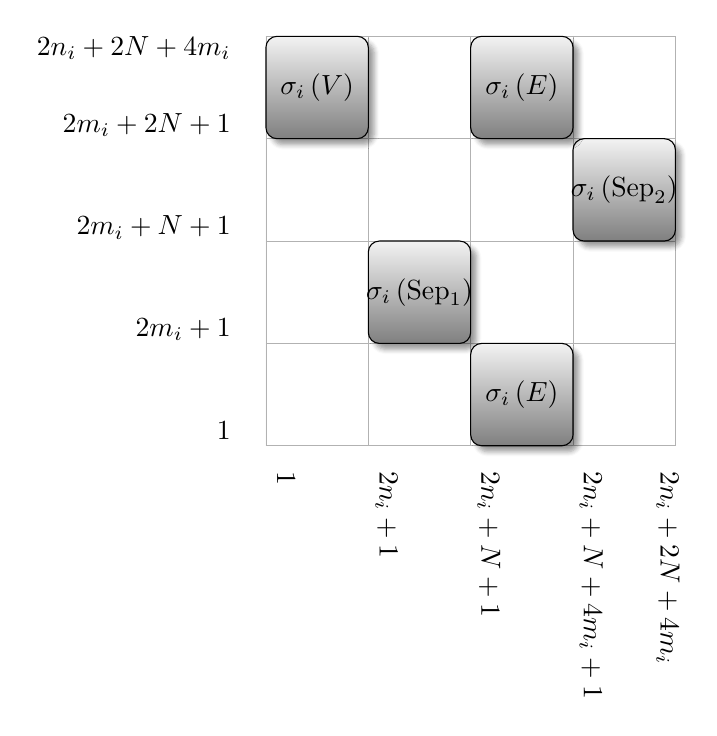
\begin{tikzpicture}
  [
    scale=.65,
    box/.style={
      shade,
      blur shadow={shadow blur steps=5,shadow blur extra rounding=1.3pt},
      top color=black!5,
      bottom color=black!50
    },
    gadget/.style={
      box,
      rounded corners
    },
    r/.style={
      box,
      draw,
      ultra thick,
    }
  ]
    \draw [help lines,step=2cm,black!30,fill=black!10] (0,0) grid (8,8);
    \draw [gadget] (0,6) rectangle ++(2,2);
    \node [] at (1,7) {$\sigma_i\left(V\right)$};
    \draw [gadget] (2,2) rectangle ++(2,2);
    \node [] at (3,3) {$\sigma_i\left(\text{Sep}_1\right)$};
    \draw [gadget] (4,0) rectangle ++(2,2);
    \node [] at (5,1) {$\sigma_i\left(E\right)$};
    \draw [gadget] (6,4) rectangle ++(2,2);
    \node [] at (7,5) {$\sigma_i\left(\text{Sep}_2\right)$};
    \draw [gadget] (4,6) rectangle ++(2,2);
    \node [] at (5,7) {$\sigma_i\left(E\right)$};
    % labels
    % x-labels
    \node [label={[text depth=1.75ex,label distance=0.2cm,rotate=-90]right:{$1$}}] at (0,0) {};
    % \node [label={[text depth=1.75ex,label distance=0.2cm,rotate=-90]right:{$2n$}}] at (1.5,0) {};
    \node [label={[text depth=1.75ex,label distance=0.2cm,rotate=-90]right:{$2n_i+1$}}] at (2,0) {};
    % \node [label={[text depth=1.75ex,label distance=0.2cm,rotate=-90]right:{$2n+kN$}}] at (3.5,0) {};
    \node [label={[text depth=1.75ex,label distance=0.2cm,rotate=-90]right:{$2n_i+N+1$}}] at (4,0) {};
    % \node [label={[text depth=1.75ex,label distance=0.2cm,rotate=-90]right:{$2n+kN+4m$}}] at (5.5,0) {};
    \node [label={[text depth=1.75ex,label distance=0.2cm,rotate=-90]right:{$2n_i+N+4m_i+1$}}] at (6,0) {};
    \node [label={[text depth=1.75ex,label distance=0.2cm,rotate=-90]right:{$2n_i+2N+4m_i$}}] at (7.5,0) {};
    % y-labels
    \node [label={[text depth=1.75ex,label distance=0.2cm]left:{$1$}}] at (0,0.1) {};
    % \node [label={[text depth=1.75ex,label distance=0.2cm]left:{$2m2$}}] at (0,1.6) {};
    \node [label={[text depth=1.75ex,label distance=0.2cm]left:{$2m_i+1$}}] at (0,2.1) {};
    % \node [label={[text depth=1.75ex,label distance=0.2cm]left:{$2m+kN$}}] at (0,3.6) {};
    \node [label={[text depth=1.75ex,label distance=0.2cm]left:{$2m_i+N+1$}}] at (0,4.1) {};
    % \node [label={[text depth=1.75ex,label distance=0.2cm]left:{$2m+2kN$}}] at (0,5.6) {};
    \node [label={[text depth=1.75ex,label distance=0.2cm]left:{$2m_i+2N+1$}}] at (0,6.1) {};
    \node [label={[text depth=1.75ex,label distance=0.2cm]left:{$2n_i+2N+4m_i$}}] at (0,7.6) {};
  \end{tikzpicture}
  \caption{\label{fig:NP2:bird eye view sigma_i}%
    Bird's-eye view of the permutation $\sigma_i$.
  }% end caption
\end{figure}


  A schematic representation of the permutation $\sigma_i$ is given in
  Figure~\ref{fig:NP2:bird eye view sigma_i}.

  Clearly our construction can be carried on in polynomial time.
  Indeed, we have
  $|\pi| = 2n + 4m + 2kN = 2n + 4m + 2k(2n+4m+1)$
  and
  $|\sigma_i| = 2n_i + 4m_i + 2N = 2n_i + 4m_i + 2(2n+4m+1)$,
  $1 \leq i \leq k$.
  We claim that the linear graph $G^0$ is
  $(G^1, G^2, \dots, G^k)$-colorable
  if and only if the permutation
  $\pi$ is $(\sigma_1, \sigma_2, \dots, \sigma_k)$-colorable.

  Suppose first that $G^0$ is $(G^1, G^2, \dots, G^k)$-colorable.
  Therefore, there exists a $k$-coloring such that
  every connected component of $G^0$ is monochromatic and,
  for every $1 \leq i \leq k$, colour $i$ induces a linear graph that is
  isomorphic to $G^i$.
  For every $1 \leq i \leq k$,
  let $v_{i_1}< v_{i_2} < \dots < v_{i_{n_i}}$ be the vertices of $G^0$ with color $i$.
  Let us now define a $k$-colouring $\varphi: [|\pi|] \to [k]$ of $\pi$ as follows.
  \begin{itemize}
    \item \textbf{Gadget $\pi(V)$}.
    For every $1 \leq j \leq n_i$,
    $\varphi(2i_j-2) = \varphi(2i_j-1) = i$
    \item \textbf{Gadget $\pi(\text{Sep}_1)$}.
    Colour the $i$-th increasing sequence $\nearrow_{N_0}$ with colour $i$.
    More formally,
    for every $2n + N_0(i-1) + 1 \leq j \leq 2n + iN_0$,
    $\varphi(j) = i$.
    \item \textbf{Gadget $\pi(E)$}.
    Let $e_{i_1} < e_{i_2} < \ldots < ae{i_{m_i}}$ be the edges of $G^0$ that connect
    vertices coloured with colour $i$.
    For every $1 \leq j \leq m_i$,
    $\varphi(2n + kN_0 + 4(i_j-1) + 1) = \varphi(2n + kN_0 + 4(i_j-1) + 2) =
    \varphi(2n + kN_0 + 4(i_j-1) + 3) = \varphi(2n + kN_0 + 4(i_j-1) + 4) = i$.
    \item \textbf{Gadget $\pi(\text{Sep}_2)$}.
    Colour the $i$-th increasing sequence $\nearrow_{N_0}$ with colour $i$.
    More formally,
    for every $2n + kN_0 + 4m + N_0(i-1) + 1 \leq j \leq 2n + kN_0 + 4m + iN_0$,
    $\varphi(j) = i$.
  \end{itemize}
  The reader is invited to check that, for every $1 \leq i \leq k$,
  the $i$-coloured pattern of $\pi$ is order-isomorphic to $\sigma_i$.

  Conversely, suppose that $\pi$ is $(\sigma_1, \sigma_2, \dots, \sigma_k)$-colorable.
  Therefore, there exists a $k$-coloring $\varphi: [2n_0 + 4m_0 + 2kN_0] \to [k]$
  such that, for every $1 \leq i \leq k$,
  the $i$-coloured pattern of $\pi$ is order-isomorphic to $\sigma_i$.
  Let us focus on $\sigma_i$ for some $1 \leq i \leq k$.
  Recall that
  $\sigma_i =
  \sigma_i(V)   \;
  \sigma_i\left(\text{Sep}_1\right) \;
  \sigma_i\left(E\right)   \;
  \sigma_i\left(\text{Sep}_1\right)$,
  where both
  $\sigma_i\left(\text{Sep}_1\right)$ and $\sigma_i\left(\text{Sep}_2\right)$
  are increasing sequence of length $N_0$.
  We now oberve that
  $N_0 > |\pi(V)| + |\pi(E)|$.
  Then it follows that
  (i) at least one element of $\pi(\text{Sep}_1)$ is coloured with
  colour $i$,
  and
  (ii) at least of element of $\pi(\text{Sep}_2)$ is coloured with
  colour $i$.
  But
  $\pi(\text{Sep}_1) \; \pi(\text{Sep}_2)$ and
  $\sigma_i\left(\text{Sep}_1\right) \; \sigma_i\left(\text{Sep}_2\right)$
  are both order-isomorphic to
  $\left(\bigominus_{\ell=1}^{k} \nearrow_N\right) \oplus \left(\bigominus_{\ell=1}^{k} \nearrow_N\right)$,
  and hence
  (i) $N$ vertices of $\pi(\text{Sep}_1)$ are coloured with
  colour $i$,
  and
  (ii) $N$ vertices of $\pi(\text{Sep}_1)$ are coloured with
  colour $i$.
  Therefore,
  (i) $|\sigma_i(V)| = 2n_i$ elements of
  $\pi(V)$ are coloured with colour $i$ and the induced
  $i$-coloured pattern is order-isomorphic to $\sigma_i(V)$,
  and
  (ii) $|\sigma_i\left(E\right)| = 4m_i$ elements of
  $\pi(E)$ are coloured with colour $i$ and the induced
  $i$-coloured pattern is order-isomorphic to $\sigma_i\left(E\right)$.
  But $\pi(V)$ is order-isomorphic to $\bigoplus_{\ell=1}^{n} 21$
  and
  $\sigma_i(V)$ is order-isomorphic to $\bigoplus_{\ell=1}^{n_i} 21$.
  Therefore, $n_i$ patterns $21$ are coloured with colour $i$ thereby identifying
  $n_i$ vertices of $G$.
  Finally,
  combining
  $\pi(E) = \bigoplus_{\ell=1}^{m} 2 \; x_\ell^1 \; x_\ell^2 \; 1$ and
  $\sigma_i\left(E\right) = \bigoplus_{\ell=1}^{m_i} 2 \; x_{i,\ell^1} \; x_{i,\ell^2} \; 1$,
  together with the fact that $x_{i,\ell^1}$ and $x_{i,\ell^2}$ have to be sandwiched in
  $i$-coloured pattern $21$ of $\pi(V)$,
  we conclude that $m_i$ consecutive patterns $2 \; x_{i,\ell^1} \; x_{i,\ell^2} \; 1$
  of $\pi(E)$ are coloured with colour $i$.
  Hence, \todo{Ok I'm lazy (or tired), this is not formal!}referring to
  Figure~\ref{fig:NP2:connection zoom} and considering every $1 \leq i \leq k$,
  we conclude that $G$ can be splitted by linear graphs $H_1, H_2, \ldots, H_k$.
  \qed
\end{proof}

\begin{corollary}
  \label{corollary:5-permutation coloring is NP-complete}
  \textsc{$3$-permutation coloring} is \NPC.
\end{corollary}

\begin{proof}
  Combine Proposition~\ref{proposition:3-Linear Graph Coloring}
  with Proposition~\ref{proposition:k-linear-graph coloring < k-permutation coloring}.
  \qed
\end{proof}

It is worth noticing that, according to
Proposition~\ref{proposition:k-linear-graph coloring < k-permutation coloring},
any improvement on Proposition~\ref{proposition:5-linear-graph coloring is NP-complete}
would immediately propagate to \textsc{$k$-permutation coloring}.


% Monotonic patterns
>>>>>>> fa71033edefafa3f3a1a458af386c80dc8565f59
\section{Monotonic permutations}
\label{section:Monotonic permutations}

\begin{proposition}
  \label{proposition:Monotonic Permutation Coloring}
  \textsc{$k$-Permutation Coloring} for monotonic permutations
  $\sigma_1, \sigma_2, \dots, \sigma_k$, $1 \leq i \leq k$, is
  solvable in $O(n^{2k+1})$ time.
\end{proposition}

\begin{proof}
  Let $(\pi \;\mid\; \sigma_1, \sigma_2, \dots, \sigma_k)$ be an instance
  of \textsc{$k$-Permutation Coloring} where every permutation
  $\sigma_1, \sigma_2, \dots, \sigma_k$, $1 \leq i \leq k$, is
  monotonic (\emph{i.e.}, either an increasing or a decreasing permutation).
  Write $n = |\pi|$.
  For every $1 \leq i \leq n$, define $T[i]$ to be set of all sequences of
  integer coordinates $2$-dimensional points
  $(p_1=(x_1, y_1), p_2=(x_2, y_2), \dots, p_k=(x_k, y_k))$,
  $\sum_{j=1}^{k} y_j = i$ and $0 \leq y_j \leq |\sigma_j|$ for $1 \leq j \leq k$,
  such that
  $\pi(1) \, \pi(2) \, \dots \, \pi(i)$ can be colored with at most $k$
  distinct colors
  with the property that every color $1 \leq j \leq k$ induces a patterns of length $y_j$
  order-isomorphic to $\sigma_j$ ($\sigma_j$ is either increasing ir decreasing)
  with rightmost element $x_j$.

  The table $T$ can be computed as follows.
  \begin{itemize}
    \item \textbf{Initialization}.
    For every $1 \leq j \leq k$,
    $$(p_1=(0,0), \dots, p_j=(\pi(1), 1), \dots, p_k=(0,0)) \in T[1]\text{.}$$

    \item \textbf{Inductive step}.
    Let $1 \leq i \leq n-1$ and
    let $((y_1, y_1) (y_2, y_2), \dots, (y_k, y_k))$ be any $k$-sequence of
    $T[i]$.
    For every $1 \leq j \leq k$,
    \begin{itemize}
      \item \textbf{$\sigma_j$ is increasing}:
      if $\pi(i) > x_j$ and $y_j < |\sigma_j|$,
      $$(p_1=(y_1, y_1), \dots, p_j=(\pi(i), y_j+1), \dots, p_k=(y_k, y_k)) \in T[i+1]\text{.}$$
      \item \textbf{$\sigma_j$ is decreasing}:
      if $\pi(i) < x_j$ and $y_j < |\sigma_j|$,
      $$(p_1=(y_1, y_1), \dots, p_j=(\pi(i), y_j+1), \dots, p_k=(y_k, y_k)) \in T[i+1]\text{.}$$
    \end{itemize}
  \end{itemize}

  For every $1 \leq i \leq n$, $T[i]$ contains $O(n^{2k})$ sequences and hence
  $T[n]$ can be computed in $O(n^{2k+1})$ time.
  \qed
\end{proof}

We now show that no significant improvement over the $n^{O(k)}$ dynamic programming algorithm
is possible for \textsc{$k$-Permutation Coloring}
for increasing patterns.

Complexity investigations usually distinguish two versions of Bin Packing. In the general
version, the item sizes are arbitrary integers encoded in binary, thus they can be exponentially
large in the size n of the input. In the unary version of the problem, the sizes are bounded by
a polynomial of the input size; formally, this version requires that the sizes are given in unary
encoding.

\begin{proposition}
  \label{proposition:Monotonic Permutation Coloring}
  \textsc{$k$-Permutation Coloring} for increasing permutations
  $\sigma_1, \sigma_2, \dots, \sigma_k$ is
  $\W[1]$-hard parameterized by $k$.
\end{proposition}

\begin{proof}
  \textsc{Unary Bin Packing} parameterized by the number of bins which is
  known to be $\W[1]$-hard \cite{DBLP:journals/jcss/JansenKMS13}.
  In this version of \textsc{Bin Packing}, we are given a set of integers
  $S = \{s_1, s_2, \dots, s_n\}$
  encoded in unary, and two integers $B$ and $k$.
  The task is to decide whether the items can be partitioned into $k$ susbets of
  total size $B$.
  We show that there is a parameterized reduction from
  \textsc{Unary Bin Packing} parameterized by the number of bins to
  \textsc{$k$-Permutation Coloring} for monotonic patterns
  parameterized by the number of monotonic patterns.

  Consider an arbitrary instance of \textsc{Unary Bin Packing} containing
  $n$ items with item sizes $S = \{s_1, s_2, \dots, s_n\}$,
  and two integers $B$ and $k$.
  We construct an instance of \textsc{$k$-Permutation Coloring}
  as follows.
  First, the target permutation $\pi$ is defined by:
  $$
  \pi =
    \bigoplus_{i=1}^{n} \left(\mathbf{\nearrow}_{s_i+1} \ominus
                              \mathbf{\searrow}_{k-1}\right)
    \text{.}
  $$
  We refer to each
  $\left(\mathbf{\nearrow}_{s_i+1} \ominus \mathbf{\searrow}_{k-1}\right)$,
  $1 \leq i \leq n$,
  as the $i$-th pattern of $\pi$.
  As for the monotonic patterns,
  define $\sigma_i = {\nearrow}_{B+n}$
  for $1 \leq i \leq k$.
  Notice that all monotonic patterns are identical;
  see Fig.~\ref{fig:bin-packing} for an illustration.

  \begin{figure}
  \centering
  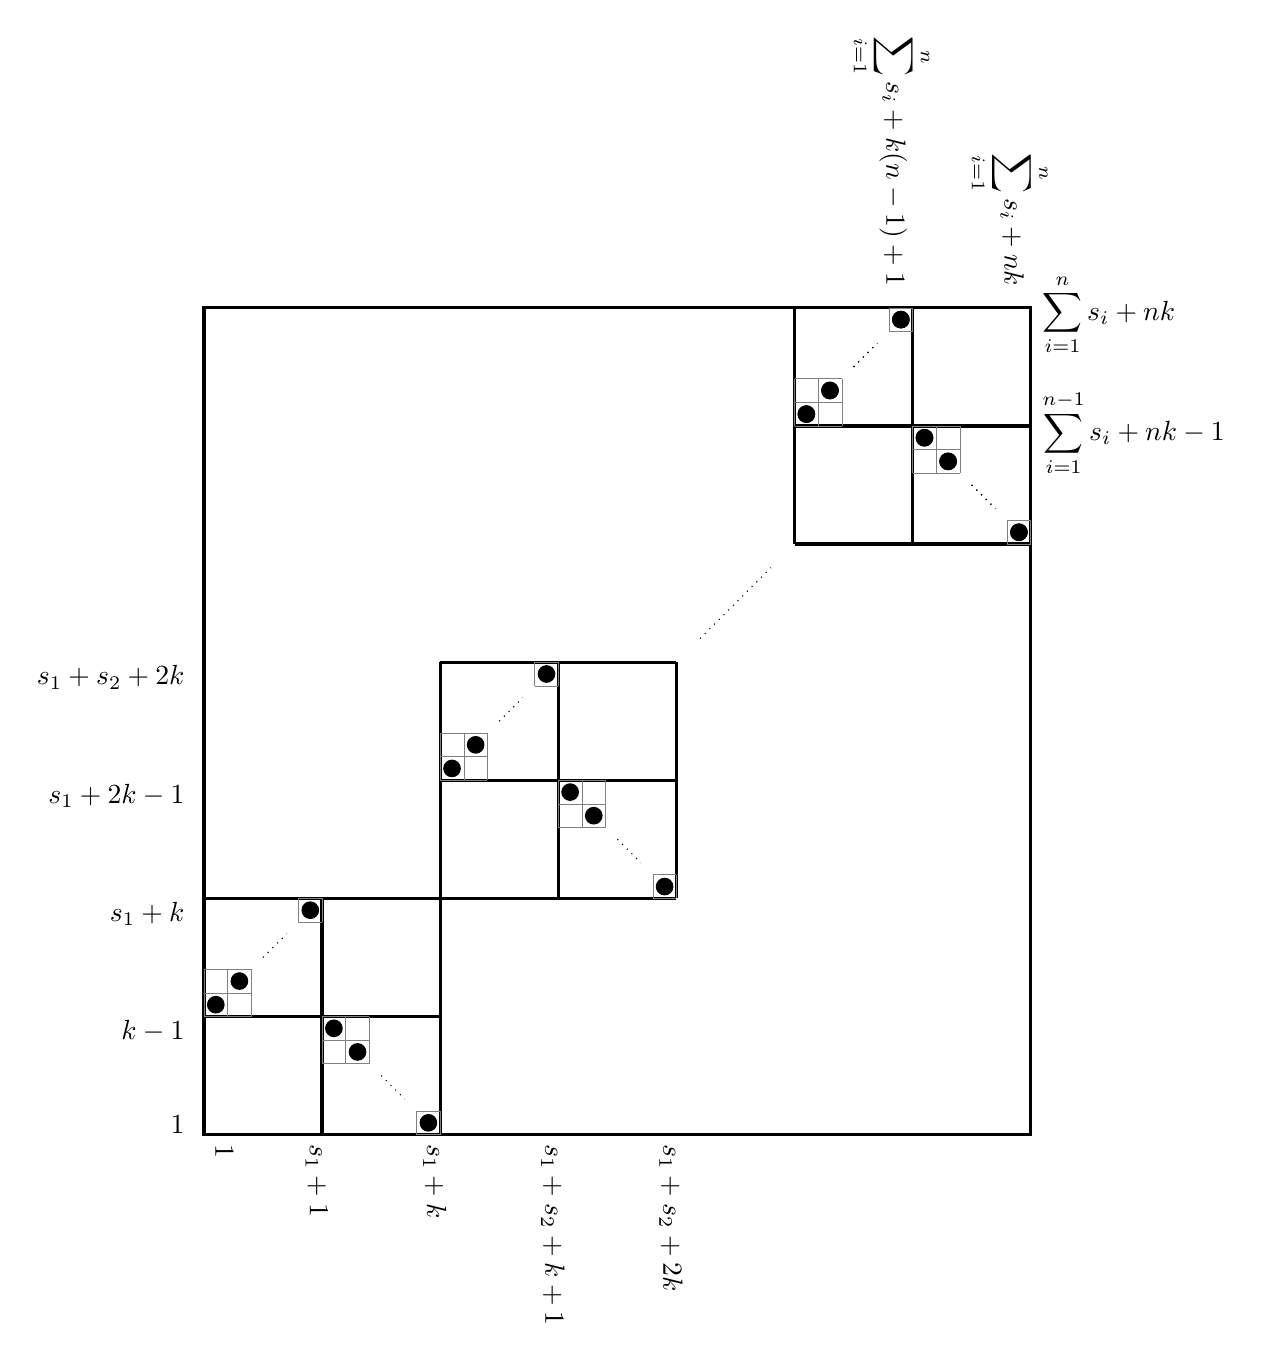
\begin{tikzpicture}
    [
      scale=.3,
    ]
    %
    \draw [black,very thick] (0, 0) rectangle (35, 35);
    \draw [step=5cm,very thick] (0, 0)   grid (10, 10);
    \draw [step=5cm,very thick] (10, 10) grid (20, 20);
    \draw [dotted] (21, 21) -- (24, 24);
    \draw [step=5cm,very thick] (25, 25) grid (35, 35);

    \foreach \x/\y in {0/0, 10/10,25,25} {
      % increasing
      \draw [black, help lines] (\x + 0, \y + 5) grid (\x + 2, \y + 7);
      \draw [black, help lines] (\x + 4, \y + 9) grid (\x + 5, \y + 10);
      \draw [black,fill=black] (\x + 1 - .5, \y + 6 -.5) circle (0.35);
      \draw [black,fill=black] (\x + 2 - .5, \y + 7 -.5) circle (0.35);
      \draw [dotted] (\x + 2.5, \y + 7.5) -- (\x + 3.5, \y + 8.5);
      \draw [black,fill=black] (\x + 5 - .5, \y + 10 -.5) circle (0.35);

      % decreasing
      \draw [black, help lines] (\x + 5, \y + 3) grid (\x + 7, \y + 5); 
      \draw [black, help lines] (\x + 9, \y + 0) grid (\x + 10, \y + 1);
      \draw [black,fill=black] (\x + 6 - .5, \y + 5 -.5) circle (0.35);
      \draw [black,fill=black] (\x + 7 - .5, \y + 4 -.5) circle (0.35);
      \draw [dotted] (\x + 7.5, \y + 2.5) -- (\x + 8.5, \y + 1.5);
      \draw [black,fill=black] (\x + 10 - .5, \y + 1 -.5) circle (0.35);
    }

    % x-labels
    \node [label={[text depth=1.75ex,label distance=0.0cm,rotate=-90]right:{$1$}}] at (0,0) {};
    \node [label={[text depth=1.75ex,label distance=0.0cm,rotate=-90]right:{$s_1+1$}}] at (4,0) {};
    \node [label={[text depth=1.75ex,label distance=0.0cm,rotate=-90]right:{$s_1+k$}}] at (9,0) {};
    \node [label={[text depth=1.75ex,label distance=0.0cm,rotate=-90]right:{$s_1+s_2+k+1$}}] at (14,0) {};
    \node [label={[text depth=1.75ex,label distance=0.0cm,rotate=-90]right:{$s_1+s_2+2k$}}] at (19,0) {};
    \node [label={[text depth=1.75ex,label distance=0.0cm,rotate=-90,anchor=east]right:{$\displaystyle\sum_{i=1}^{n}s_i+k(n-1)+1$}}] at (29,35.5) {};
    \node [label={[text depth=1.75ex,label distance=0.0cm,rotate=-90,anchor=east]right:{$\displaystyle\sum_{i=1}^{n}s_i+nk$}}] at (34,35.5) {};

    % y labels
    \node [label={[text depth=1.75ex,label distance=0.0cm,anchor=east]left:{$1$}}] at (0, 0) {};
    \node [label={[text depth=1.75ex,label distance=0.0cm,anchor=east]left:{$k-1$}}] at (0, 4) {};
    \node [label={[text depth=1.75ex,label distance=0.0cm,anchor=east]left:{$s_1+k$}}] at (0, 9) {};
    \node [label={[text depth=1.75ex,label distance=0.0cm,anchor=east]left:{$s_1+2k-1$}}] at (0, 14) {};
    \node [label={[text depth=1.75ex,label distance=0.0cm,anchor=east]left:{$s_1+s_2+2k$}}] at (0, 19) {};
    \node [label={[text depth=1.75ex,label distance=0.0cm,anchor=west]left:{$\displaystyle\sum_{i=1}^{n-1}s_i+nk-1$}}] at (35.5, 30) {};
    \node [label={[text depth=1.75ex,label distance=0.0cm,anchor=west]left:{$\displaystyle\sum_{i=1}^{n}s_i+nk$}}] at (35.5,35) {};
  \end{tikzpicture}
  \caption{\label{fig:bin-packing}%
  \textsc{Bin Packing}.}
\end{figure}


  We claim that the $n$ items $s_1, s_2, \dots, s_n$
  can be partitioned into $k$ susbets, each of total size $B$,
  if and only if
  $\pi$ can be colored by $k$ increasing permutations of length $B+n$.

  $(\Rightarrow)$
  Suppose that the $n$ items $s_1, s_2, \dots, s_n$
  can be partitioned into $k$ susbets, each of total size $B$.
  Write $S = S_1 \cup S_2 \cup \dots \cup S_k$ such a partition.
  Define a $k$-coloring of $\pi$ as follows.
  Consider any
  $\left(\mathbf{\nearrow}_{s_i+1} \ominus \mathbf{\searrow}_{k-1}\right)$
  pattern of $\pi$,
  and suppose that $s_i \in S_j$.
  Color the whole ascending pattern $\mathbf{\nearrow}_{s_i+1}$ with color $c_j$
  and color arbitrarily the elements of the descending pattern
  $\mathbf{\searrow}_{k-1}$ with the remaining $k-1$ colors
  (each element of $\mathbf{\searrow}_{k-1}$ is assigning a distinct color).
  We claim that every color $c_j$, $1 \leq j \leq k$, induces an increasing pattern
  of length $B+n$ in $\pi$.
  First, it is clear that the above $k$-coloring induces increasing patterns only.
  As for the length of each induced increasing pattern, focus on any color
  $c_j$, $1 \leq j \leq k$.
  We note that in every
  $\left(\mathbf{\nearrow}_{s_i+1} \ominus \mathbf{\searrow}_{k-1}\right)$
  pattern of $\pi$, either the whole $\mathbf{\nearrow}_{s_i+1}$ subpattern is
  colored with color $c_j$ (if $s_i \in S_j$) or exactly one element of the
  $\mathbf{\searrow}_{k-1}$ subpattern is colored with color $c_j$
  (if $s_i \notin S_j$).
  Then it follows that the increasing pattern induced by color $c_j$ in $\pi$ has
  length
  $\sum_{s_i \in S_j} \left(s_i + 1\right) + n - |S_i|
  =
  \sum_{s_i \in S_j} s_i + |S_i| + n - |S_i|
  = B + n$.

  $(\Leftarrow)$
  Suppose now that there exists a $k$-coloring of $\pi$ such that each color
  induces
  an increasing pattern of length $B+n$.
  Observe that every
  $\left(\mathbf{\nearrow}_{s_i+1} \ominus \mathbf{\searrow}_{k-1}\right)$
  pattern requires at least $k$ colors as it contains a decreasing subpattern of
  length $k$.
  Therefore the whole $\mathbf{\nearrow}_{s_i+1}$ subpattern is colored with the
  same color.
  For every $1 \leq j \leq k$, define $S_j$ to be the set of all $s_i$ such that
  in the $i$-th
  $\left(\mathbf{\nearrow}_{s_i+1} \ominus \mathbf{\searrow}_{k-1}\right)$
  pattern, the $\mathbf{\nearrow}_{s_i+1}$ subpattern is colored with color $c_j$.
  Therefore, for every $1 \leq j \leq k$, we have
  $B + n = \sum_{s_i \in S_j} \left(s_i+1\right) + n - |S_j|
  = \sum_{s_i \in S_j} s_i + |S_j| + n - |S_j|$,
  and hence
  $\sum_{s_i \in S_j} s_i = B$.
  Therefore, the $n$ items $s_1, s_2, \dots, s_n$
  can be packed into $k$ bins, each of capacity $B$.
\end{proof}


% Concluding remarks
\section{Conclusion}
\label{section:Conclusion}

The rationale for introducing \textsc{$k$-Permutation Coloring} stems
from square permutations (\emph{i.e.} those permutations $\pi$ that are
$(\sigma, \sigma)$-colorable for some $\sigma$).
Given a permutation $\pi$, it is \NP-complete to decide
whether there exists some permutations $\sigma$ such that
$\pi \in \sigma \bullet \sigma$ \cite{DBLP:journals/tcs/GiraudoV18}.
How hard becomes the problem if $\sigma$ is part of the input ?
In other words, given permutation $\pi$ and $\sigma$, how hard is the problem
to deciding whether $\sigma$ is a square root
of $\pi$?


%%%%%%%%%%%%%%%%%%%%%%%%%%%%%%%%%%%%%%%%%%%%%%%%%%%%%%%%%%%%%%%%%%%%%%%%%%%%%%%

%\bibliographystyle{amsplain}
\bibliography{biblio}

%%%%%%%%%%%%%%%%%%%%%%%%%%%%%%%%%%%%%%%%%%%%%%%%%%%%%%%%%%%%%%%%%%%%%%%%%%%%%%%%%%%%%%

\end{document}

%%%%%%%%%%%%%%%%%%%%%%%%%%%%%%%%%%%%%%%%%%%%%%%%%%%%%%%%%%%%%%%%%%%%%%%%%%%%%%%
